\documentclass[a4paper]{book}
\usepackage{makeidx}
\usepackage{natbib}
\usepackage{graphicx}
\usepackage{multicol}
\usepackage{float}
\usepackage{listings}
\usepackage{color}
\usepackage{ifthen}
\usepackage[table]{xcolor}
\usepackage{textcomp}
\usepackage{alltt}
\usepackage{ifpdf}
\ifpdf
\usepackage[pdftex,
            pagebackref=true,
            colorlinks=true,
            linkcolor=blue,
            unicode
           ]{hyperref}
\else
\usepackage[ps2pdf,
            pagebackref=true,
            colorlinks=true,
            linkcolor=blue,
            unicode
           ]{hyperref}
\usepackage{pspicture}
\fi
\usepackage[utf8]{inputenc}
\usepackage{mathptmx}
\usepackage[scaled=.90]{helvet}
\usepackage{courier}
\usepackage{sectsty}
\usepackage[titles]{tocloft}
\usepackage{doxygen}
\lstset{language=C++,inputencoding=utf8,basicstyle=\footnotesize,breaklines=true,breakatwhitespace=true,tabsize=8,numbers=left }
\makeindex
\setcounter{tocdepth}{3}
\renewcommand{\footrulewidth}{0.4pt}
\renewcommand{\familydefault}{\sfdefault}
\hfuzz=15pt
\setlength{\emergencystretch}{15pt}
\hbadness=750
\tolerance=750
\begin{document}
\hypersetup{pageanchor=false,citecolor=blue}
\begin{titlepage}
\vspace*{7cm}
\begin{center}
{\Large nebula }\\
\vspace*{1cm}
{\large \-Generated by Doxygen 1.7.6.1}\\
\vspace*{0.5cm}
{\small Tue Apr 22 2014 21:51:40}\\
\end{center}
\end{titlepage}
\clearemptydoublepage
\pagenumbering{roman}
\tableofcontents
\clearemptydoublepage
\pagenumbering{arabic}
\hypersetup{pageanchor=true,citecolor=blue}
\chapter{\-Todo \-List}
\label{todo}
\hypertarget{todo}{}

\begin{DoxyRefList}
\item[\label{todo__todo000011}%
\hypertarget{todo__todo000011}{}%
\-Member \hyperlink{classgal_1_1network_1_1communicating_abd5efaa6563dda2097f69ae3679f87a1}{gal\-:\-:network\-:\-:communicating\-:\-:thread\-\_\-read} ()]pass exception to main thread ( or whoever )  
\item[\label{todo__todo000010}%
\hypertarget{todo__todo000010}{}%
\-Member \hyperlink{classgal_1_1network_1_1communicating_a271caa9e5d4d13fffda9d38218231b2c}{gal\-:\-:network\-:\-:communicating\-:\-:thread\-\_\-write} (boost\-::shared\-\_\-ptr$<$ message $>$)]pass exception to main thread ( or whoever )  
\item[\label{todo__todo000008}%
\hypertarget{todo__todo000008}{}%
\-Class \hyperlink{structglutpp_1_1network_1_1actor_1_1update_1_1addr__raw}{glutpp\-:\-:network\-:\-:actor\-:\-:update\-:\-:addr\-\_\-raw} ]find a way to implement this using \-Wrapper\-Typed or somehting like it  
\item[\label{todo__todo000009}%
\hypertarget{todo__todo000009}{}%
\-Member \hyperlink{structglutpp_1_1network_1_1actor_1_1update_1_1addr__raw_a4883db7c0b5227e0fcb124f786a121c1}{glutpp\-:\-:network\-:\-:actor\-:\-:update\-:\-:addr\-\_\-raw\-:\-:load} (\-Archive \&ar, unsigned int const \&version)]handle this gracefully  
\item[\label{todo__todo000007}%
\hypertarget{todo__todo000007}{}%
\-Member \hyperlink{structglutpp_1_1network_1_1actor_1_1update_a2a7bee8209aa582266f5bb4e6e729501}{glutpp\-:\-:network\-:\-:actor\-:\-:update\-:\-:load} (\-Neb\-::weak\-\_\-ptr$<$ glutpp\-::actor\-::actor $>$ const \&actor)]this and all similar functions should be not be called \char`\"{}load\char`\"{}, in fact, they are used on the \char`\"{}save\char`\"{} side of the serialization process. if anything, call them save.  
\item[\label{todo__todo000006}%
\hypertarget{todo__todo000006}{}%
\-Namespace \hyperlink{namespaceNeb}{\-Neb} ]under what conditions is it necessary to 

replace types with inheritance and possibly shared library support  
\item[\label{todo__todo000001}%
\hypertarget{todo__todo000001}{}%
\-Member \hyperlink{classNeb_1_1app_acefbc3bb3de71f3c8cca0afc1fada857}{\-Neb\-:\-:app\-:\-:recv\-\_\-scene\-\_\-create} (std\-::shared\-\_\-ptr$<$ gal\-::network\-::message $>$)]consider putting following functions into the messages themselves\-: would be cleaner that way.  
\item[\label{todo__todo000003}%
\hypertarget{todo__todo000003}{}%
\-Member \hyperlink{classNeb_1_1Camera_1_1Projection_1_1Base_a7a0ef0507f546a0da56bb596de53c962}{\-Neb\-:\-:\-Camera\-:\-:\-Projection\-:\-:\-Base\-:\-:step} (double)]explain when in timeline this occurs and in which thread and why  
\item[\label{todo__todo000004}%
\hypertarget{todo__todo000004}{}%
\-Member \hyperlink{classNeb_1_1Camera_1_1View_1_1Base_aa3c5978efc6cd916f0f91bb8def375c5}{\-Neb\-:\-:\-Camera\-:\-:\-View\-:\-:\-Base\-:\-:step} (double)=0]explain when in timeline this occurs and in which thread and why  
\item[\label{todo__todo000012}%
\hypertarget{todo__todo000012}{}%
\-Class \hyperlink{classNeb_1_1renderable}{\-Neb\-:\-:renderable} ]eventually replace this with \-Context and allow multiple \-Contexts per window and allow scene and layout to have different and overalpping \-Contexts.  
\item[\label{todo__todo000013}%
\hypertarget{todo__todo000013}{}%
\-Member \hyperlink{classNeb_1_1Scene_1_1desc_aa456a9a431a4f93be8278f6aee75b8f6}{\-Neb\-:\-:\-Scene\-:\-:desc\-:\-:serialize} (\-Archive \&ar, unsigned int const \&version)]no idea why this fails  
\item[\label{todo__todo000016}%
\hypertarget{todo__todo000016}{}%
\-Member \hyperlink{classNeb_1_1Shape_1_1desc_a8356295ceee1f17dd24afbdb455dd206}{\-Neb\-:\-:\-Shape\-:\-:desc\-:\-:operator$<$$<$} (\-Neb\-::\-Shape\-::shape\-\_\-w const \&)]fill this out  
\item[\label{todo__todo000005}%
\hypertarget{todo__todo000005}{}%
\-Member \hyperlink{classNeb_1_1window_1_1window_a04992828fdcd620216728e607654e26a}{\-Neb\-:\-:window\-:\-:window\-:\-:window} (\-Neb\-::window\-::desc\-\_\-s desc)]get rid of my unique ptr class. \-Just use private member and be careful not to pass around shared ptrs to things 
\end{DoxyRefList}
\chapter{\-Namespace \-Index}
\section{Namespace List}
Here is a list of all documented namespaces with brief descriptions:\begin{DoxyCompactList}
\item\contentsline{section}{\hyperlink{namespaceneb}{neb} (Nebula )}{\pageref{namespaceneb}}{}
\item\contentsline{section}{\hyperlink{namespaceneb_1_1Actor}{neb::Actor} (Actor )}{\pageref{namespaceneb_1_1Actor}}{}
\item\contentsline{section}{\hyperlink{namespaceneb_1_1control}{neb::control} (Control )}{\pageref{namespaceneb_1_1control}}{}
\item\contentsline{section}{\hyperlink{namespaceneb_1_1network}{neb::network} (Network )}{\pageref{namespaceneb_1_1network}}{}
\item\contentsline{section}{\hyperlink{namespaceneb_1_1scene}{neb::scene} (Scene )}{\pageref{namespaceneb_1_1scene}}{}
\item\contentsline{section}{\hyperlink{namespaceneb_1_1shape}{neb::shape} (Shape )}{\pageref{namespaceneb_1_1shape}}{}
\item\contentsline{section}{\hyperlink{namespaceneb_1_1timer}{neb::timer} (Timer )}{\pageref{namespaceneb_1_1timer}}{}
\end{DoxyCompactList}

\chapter{\-Class \-Index}
\section{\-Class \-Hierarchy}
\-This inheritance list is sorted roughly, but not completely, alphabetically\-:\begin{DoxyCompactList}
\item \contentsline{section}{\-Neb\-:\-:\-Func\-Map\-:\-:\-\_\-\-\_\-base\-\_\-function}{\pageref{structNeb_1_1FuncMap_1_1____base__function}}{}
\begin{DoxyCompactList}
\item \contentsline{section}{\-Neb\-:\-:\-Func\-Map\-:\-:\-\_\-\-\_\-function$<$ \-R, \-A $>$}{\pageref{structNeb_1_1FuncMap_1_1____function}}{}
\end{DoxyCompactList}
\item \contentsline{section}{neb\-:\-:packet\-:\-:actor\-\_\-release}{\pageref{classneb_1_1packet_1_1actor__release}}{}
\item \contentsline{section}{\-Neb\-:\-:\-Scene\-:\-:\-Util\-:\-:\-Address}{\pageref{classNeb_1_1Scene_1_1Util_1_1Address}}{}
\item \contentsline{section}{\-Neb\-:\-:\-Util\-:\-:\-Address$<$ \-T $>$}{\pageref{classNeb_1_1Util_1_1Address}}{}
\item \contentsline{section}{\-Neb\-:\-:\-Actor\-:\-:\-Util\-:\-:\-Address}{\pageref{classNeb_1_1Actor_1_1Util_1_1Address}}{}
\item \contentsline{section}{\-Neb\-:\-:\-Util\-:\-:\-Address\-Base}{\pageref{classNeb_1_1Util_1_1AddressBase}}{}
\item \contentsline{section}{\-Archive\-Read}{\pageref{classArchiveRead}}{}
\item \contentsline{section}{\-Neb\-:\-:glsl\-:\-:attrib}{\pageref{classNeb_1_1glsl_1_1attrib}}{}
\item \contentsline{section}{\-Neb\-:\-:attrib\-\_\-name}{\pageref{structNeb_1_1attrib__name}}{}
\item \contentsline{section}{\-Neb\-:\-:glsl\-:\-:\-Uniform\-:\-:\-Scalar\-:\-:\-Base}{\pageref{classNeb_1_1glsl_1_1Uniform_1_1Scalar_1_1Base}}{}
\begin{DoxyCompactList}
\item \contentsline{section}{\-Neb\-:\-:glsl\-:\-:\-Uniform\-:\-:\-Scalar\-:\-:\-Double}{\pageref{classNeb_1_1glsl_1_1Uniform_1_1Scalar_1_1Double}}{}
\item \contentsline{section}{\-Neb\-:\-:glsl\-:\-:\-Uniform\-:\-:\-Scalar\-:\-:\-D\-Vec4}{\pageref{classNeb_1_1glsl_1_1Uniform_1_1Scalar_1_1DVec4}}{}
\item \contentsline{section}{\-Neb\-:\-:glsl\-:\-:\-Uniform\-:\-:\-Scalar\-:\-:\-Float}{\pageref{classNeb_1_1glsl_1_1Uniform_1_1Scalar_1_1Float}}{}
\item \contentsline{section}{\-Neb\-:\-:glsl\-:\-:\-Uniform\-:\-:\-Scalar\-:\-:\-Int}{\pageref{classNeb_1_1glsl_1_1Uniform_1_1Scalar_1_1Int}}{}
\item \contentsline{section}{\-Neb\-:\-:glsl\-:\-:\-Uniform\-:\-:\-Scalar\-:\-:\-Mat4}{\pageref{classNeb_1_1glsl_1_1Uniform_1_1Scalar_1_1Mat4}}{}
\item \contentsline{section}{\-Neb\-:\-:glsl\-:\-:\-Uniform\-:\-:\-Scalar\-:\-:\-Sampler2\-D}{\pageref{classNeb_1_1glsl_1_1Uniform_1_1Scalar_1_1Sampler2D}}{}
\item \contentsline{section}{\-Neb\-:\-:glsl\-:\-:\-Uniform\-:\-:\-Scalar\-:\-:\-Vec3}{\pageref{classNeb_1_1glsl_1_1Uniform_1_1Scalar_1_1Vec3}}{}
\item \contentsline{section}{\-Neb\-:\-:glsl\-:\-:\-Uniform\-:\-:\-Scalar\-:\-:\-Vec4}{\pageref{classNeb_1_1glsl_1_1Uniform_1_1Scalar_1_1Vec4}}{}
\end{DoxyCompactList}
\item \contentsline{section}{\-Neb\-:\-:\-Message\-:\-:\-Base}{\pageref{classNeb_1_1Message_1_1Base}}{}
\begin{DoxyCompactList}
\item \contentsline{section}{\-Neb\-:\-:\-Message\-:\-:\-Actor\-:\-:\-Base}{\pageref{classNeb_1_1Message_1_1Actor_1_1Base}}{}
\begin{DoxyCompactList}
\item \contentsline{section}{\-Neb\-:\-:\-Message\-:\-:\-Actor\-:\-:\-Control\-:\-:\-Rigid\-Body\-:\-:\-Create}{\pageref{classNeb_1_1Message_1_1Actor_1_1Control_1_1RigidBody_1_1Create}}{}
\item \contentsline{section}{\-Neb\-:\-:\-Message\-:\-:\-Actor\-:\-:\-Event}{\pageref{classNeb_1_1Message_1_1Actor_1_1Event}}{}
\item \contentsline{section}{\-Neb\-:\-:\-Message\-:\-:\-Actor\-:\-:\-I\-Base}{\pageref{classNeb_1_1Message_1_1Actor_1_1IBase}}{}
\begin{DoxyCompactList}
\item \contentsline{section}{\-Neb\-:\-:\-Message\-:\-:\-Actor\-:\-:\-Control\-:\-:\-Rigid\-Body\-:\-:\-I\-Update}{\pageref{classNeb_1_1Message_1_1Actor_1_1Control_1_1RigidBody_1_1IUpdate}}{}
\end{DoxyCompactList}
\item \contentsline{section}{\-Neb\-:\-:\-Message\-:\-:\-Actor\-:\-:\-O\-Base}{\pageref{classNeb_1_1Message_1_1Actor_1_1OBase}}{}
\begin{DoxyCompactList}
\item \contentsline{section}{\-Neb\-:\-:\-Message\-:\-:\-Actor\-:\-:\-Control\-:\-:\-Rigid\-Body\-:\-:\-O\-Update}{\pageref{classNeb_1_1Message_1_1Actor_1_1Control_1_1RigidBody_1_1OUpdate}}{}
\end{DoxyCompactList}
\end{DoxyCompactList}
\item \contentsline{section}{\-Neb\-:\-:\-Message\-:\-:\-Actor\-:\-:\-Update}{\pageref{structNeb_1_1Message_1_1Actor_1_1Update}}{}
\begin{DoxyCompactList}
\item \contentsline{section}{\-Neb\-:\-:\-Message\-:\-:\-Actor\-:\-:\-I\-Update}{\pageref{structNeb_1_1Message_1_1Actor_1_1IUpdate}}{}
\item \contentsline{section}{\-Neb\-:\-:\-Message\-:\-:\-Actor\-:\-:\-O\-Update}{\pageref{structNeb_1_1Message_1_1Actor_1_1OUpdate}}{}
\end{DoxyCompactList}
\item \contentsline{section}{\-Neb\-:\-:\-Message\-:\-:\-I\-Base}{\pageref{classNeb_1_1Message_1_1IBase}}{}
\begin{DoxyCompactList}
\item \contentsline{section}{\-Neb\-:\-:\-Message\-:\-:\-Actor\-:\-:\-I\-Update}{\pageref{structNeb_1_1Message_1_1Actor_1_1IUpdate}}{}
\end{DoxyCompactList}
\item \contentsline{section}{\-Neb\-:\-:\-Message\-:\-:\-O\-Base}{\pageref{classNeb_1_1Message_1_1OBase}}{}
\begin{DoxyCompactList}
\item \contentsline{section}{\-Neb\-:\-:\-Message\-:\-:\-Actor\-:\-:\-O\-Update}{\pageref{structNeb_1_1Message_1_1Actor_1_1OUpdate}}{}
\end{DoxyCompactList}
\end{DoxyCompactList}
\item \contentsline{section}{gal\-:\-:network\-:\-:base}{\pageref{classgal_1_1network_1_1base}}{}
\item \contentsline{section}{\-Neb\-:\-:glsl\-:\-:\-Uniform\-:\-:\-Vector\-:\-:\-Base}{\pageref{classNeb_1_1glsl_1_1Uniform_1_1Vector_1_1Base}}{}
\begin{DoxyCompactList}
\item \contentsline{section}{\-Neb\-:\-:glsl\-:\-:\-Uniform\-:\-:\-Vector\-:\-:\-Double}{\pageref{classNeb_1_1glsl_1_1Uniform_1_1Vector_1_1Double}}{}
\item \contentsline{section}{\-Neb\-:\-:glsl\-:\-:\-Uniform\-:\-:\-Vector\-:\-:\-D\-Vec3}{\pageref{classNeb_1_1glsl_1_1Uniform_1_1Vector_1_1DVec3}}{}
\item \contentsline{section}{\-Neb\-:\-:glsl\-:\-:\-Uniform\-:\-:\-Vector\-:\-:\-D\-Vec4}{\pageref{classNeb_1_1glsl_1_1Uniform_1_1Vector_1_1DVec4}}{}
\item \contentsline{section}{\-Neb\-:\-:glsl\-:\-:\-Uniform\-:\-:\-Vector\-:\-:\-Float}{\pageref{classNeb_1_1glsl_1_1Uniform_1_1Vector_1_1Float}}{}
\item \contentsline{section}{\-Neb\-:\-:glsl\-:\-:\-Uniform\-:\-:\-Vector\-:\-:\-Int}{\pageref{classNeb_1_1glsl_1_1Uniform_1_1Vector_1_1Int}}{}
\item \contentsline{section}{\-Neb\-:\-:glsl\-:\-:\-Uniform\-:\-:\-Vector\-:\-:\-Vec3}{\pageref{classNeb_1_1glsl_1_1Uniform_1_1Vector_1_1Vec3}}{}
\item \contentsline{section}{\-Neb\-:\-:glsl\-:\-:\-Uniform\-:\-:\-Vector\-:\-:\-Vec4}{\pageref{classNeb_1_1glsl_1_1Uniform_1_1Vector_1_1Vec4}}{}
\end{DoxyCompactList}
\item \contentsline{section}{\-Neb\-:\-:\-Shape\-:\-:\-Event\-:\-:\-Base}{\pageref{classNeb_1_1Shape_1_1Event_1_1Base}}{}
\item \contentsline{section}{\-Neb\-:\-:\-Timer\-:\-:\-Actor\-:\-:\-Base}{\pageref{classNeb_1_1Timer_1_1Actor_1_1Base}}{}
\begin{DoxyCompactList}
\item \contentsline{section}{neb\-:\-:\-Timer\-:\-:\-Actor\-:\-:\-Release}{\pageref{classneb_1_1Timer_1_1Actor_1_1Release}}{}
\end{DoxyCompactList}
\item \contentsline{section}{\-Neb\-:\-:\-Graphics\-:\-:\-Camera\-:\-:\-Projection\-:\-:\-Base}{\pageref{classNeb_1_1Graphics_1_1Camera_1_1Projection_1_1Base}}{}
\begin{DoxyCompactList}
\item \contentsline{section}{\-Neb\-:\-:\-Graphics\-:\-:\-Camera\-:\-:\-Projection\-:\-:\-Perspective}{\pageref{classNeb_1_1Graphics_1_1Camera_1_1Projection_1_1Perspective}}{}
\end{DoxyCompactList}
\item \contentsline{section}{\-Neb\-:\-:\-Graphics\-:\-:\-Camera\-:\-:\-View\-:\-:\-Base}{\pageref{classNeb_1_1Graphics_1_1Camera_1_1View_1_1Base}}{}
\begin{DoxyCompactList}
\item \contentsline{section}{\-Neb\-:\-:\-Graphics\-:\-:\-Camera\-:\-:\-View\-:\-:\-Free}{\pageref{classNeb_1_1Graphics_1_1Camera_1_1View_1_1Free}}{}
\item \contentsline{section}{\-Neb\-:\-:\-Graphics\-:\-:\-Camera\-:\-:\-View\-:\-:\-Ridealong}{\pageref{classNeb_1_1Graphics_1_1Camera_1_1View_1_1Ridealong}}{}
\end{DoxyCompactList}
\item \contentsline{section}{\-Neb\-:\-:\-Event\-:\-:\-Actor\-:\-:\-Base}{\pageref{classNeb_1_1Event_1_1Actor_1_1Base}}{}
\item \contentsline{section}{\-Neb\-:\-:\-Actor\-:\-:\-Control\-:\-:\-Rigid\-Body\-:\-:\-Base}{\pageref{classNeb_1_1Actor_1_1Control_1_1RigidBody_1_1Base}}{}
\begin{DoxyCompactList}
\item \contentsline{section}{\-Neb\-:\-:\-Actor\-:\-:\-Control\-:\-:\-Rigid\-Body\-:\-:\-Manual}{\pageref{classNeb_1_1Actor_1_1Control_1_1RigidBody_1_1Manual}}{}
\item \contentsline{section}{\-Neb\-:\-:\-Actor\-:\-:\-Control\-:\-:\-Rigid\-Body\-:\-:\-P\-D}{\pageref{classNeb_1_1Actor_1_1Control_1_1RigidBody_1_1PD}}{}
\end{DoxyCompactList}
\item \contentsline{section}{\-Neb\-:\-:\-App\-:\-:\-Base\-Factory}{\pageref{classNeb_1_1App_1_1BaseFactory}}{}
\begin{DoxyCompactList}
\item \contentsline{section}{\-Neb\-:\-:\-App\-:\-:\-Base}{\pageref{classNeb_1_1App_1_1Base}}{}
\end{DoxyCompactList}
\item \contentsline{section}{glutpp\-:\-:buffer}{\pageref{classglutpp_1_1buffer}}{}
\item \contentsline{section}{\-Neb\-:\-:\-Shape\-:\-:buffer}{\pageref{classNeb_1_1Shape_1_1buffer}}{}
\item \contentsline{section}{neb\-:\-:camera\-:\-:camera}{\pageref{classneb_1_1camera_1_1camera}}{}
\item \contentsline{section}{\-Neb\-:\-:\-Graphics\-:\-:\-Window\-:\-:\-Util\-:\-:\-Cast}{\pageref{classNeb_1_1Graphics_1_1Window_1_1Util_1_1Cast}}{}
\begin{DoxyCompactList}
\item \contentsline{section}{\-Neb\-:\-:\-Graphics\-:\-:\-Window\-:\-:\-Base}{\pageref{classNeb_1_1Graphics_1_1Window_1_1Base}}{}
\end{DoxyCompactList}
\item \contentsline{section}{\-Neb\-:\-:\-Color\-:\-:color$<$ \-T $>$}{\pageref{classNeb_1_1Color_1_1color}}{}
\item \contentsline{section}{gal\-:\-:network\-:\-:communicating}{\pageref{classgal_1_1network_1_1communicating}}{}
\begin{DoxyCompactList}
\item \contentsline{section}{gal\-:\-:network\-:\-:client}{\pageref{classgal_1_1network_1_1client}}{}
\begin{DoxyCompactList}
\item \contentsline{section}{\-Neb\-:\-:\-Network\-:\-:\-Client}{\pageref{classNeb_1_1Network_1_1Client}}{}
\end{DoxyCompactList}
\item \contentsline{section}{\-Neb\-:\-:\-Network\-:\-:\-Communicating}{\pageref{classNeb_1_1Network_1_1Communicating}}{}
\begin{DoxyCompactList}
\item \contentsline{section}{\-Neb\-:\-:\-Network\-:\-:\-Client}{\pageref{classNeb_1_1Network_1_1Client}}{}
\end{DoxyCompactList}
\end{DoxyCompactList}
\item \contentsline{section}{\-Neb\-:\-:\-Message\-:\-:\-Scene\-:\-:\-Create}{\pageref{structNeb_1_1Message_1_1Scene_1_1Create}}{}
\item \contentsline{section}{\-Neb\-:\-:\-Message\-:\-:\-Actor\-:\-:\-Create}{\pageref{structNeb_1_1Message_1_1Actor_1_1Create}}{}
\item \contentsline{section}{\-Neb\-:\-:\-Filter\-:\-:\-Data}{\pageref{classNeb_1_1Filter_1_1Data}}{}
\item \contentsline{section}{\-Default\-Error\-Callback}{\pageref{classDefaultErrorCallback}}{}
\item \contentsline{section}{\-Neb\-:\-:\-Util\-:\-:dispatch\-\_\-init}{\pageref{structNeb_1_1Util_1_1dispatch__init}}{}
\item \contentsline{section}{\-Neb\-:\-:\-Util\-:\-:dispatch\-\_\-step}{\pageref{structNeb_1_1Util_1_1dispatch__step}}{}
\item \contentsline{section}{math\-:\-:\-Color\-:\-:\-Dynamic$<$ \-T, \-R, \-G, \-B $>$}{\pageref{classmath_1_1Color_1_1Dynamic}}{}
\item \contentsline{section}{\-Neb\-:\-:file\-\_\-header}{\pageref{structNeb_1_1file__header}}{}
\item \contentsline{section}{\-Neb\-:\-:\-Filter\-:\-:\-Filter}{\pageref{structNeb_1_1Filter_1_1Filter}}{}
\item \contentsline{section}{\-Neb\-:\-:\-Event\-:\-:\-Actor\-:\-:\-Fire}{\pageref{classNeb_1_1Event_1_1Actor_1_1Fire}}{}
\item \contentsline{section}{\-Neb\-:\-:\-App\-:\-:\-Base\-:\-:flag}{\pageref{structNeb_1_1App_1_1Base_1_1flag}}{}
\item \contentsline{section}{\-Neb\-:\-:\-Shape\-:\-:flag}{\pageref{structNeb_1_1Shape_1_1flag}}{}
\item \contentsline{section}{gal\-:\-:flag}{\pageref{classgal_1_1flag}}{}
\item \contentsline{section}{\-Neb\-:\-:\-Graphics\-:\-:\-Window\-:\-:\-Base\-:\-:flag}{\pageref{structNeb_1_1Graphics_1_1Window_1_1Base_1_1flag}}{}
\item \contentsline{section}{\-Neb\-:\-:\-Graphics\-:\-:\-Camera\-:\-:\-View\-:\-:\-Free\-:\-:\-Flag}{\pageref{structNeb_1_1Graphics_1_1Camera_1_1View_1_1Free_1_1Flag}}{}
\item \contentsline{section}{\-Neb\-:\-:\-Func\-Map}{\pageref{classNeb_1_1FuncMap}}{}
\begin{DoxyCompactList}
\item \contentsline{section}{\-Neb\-:\-:\-Factory$<$ \-T $>$}{\pageref{classNeb_1_1Factory}}{}
\item \contentsline{section}{\-Neb\-:\-:\-Initializer$<$ \-T $>$}{\pageref{classNeb_1_1Initializer}}{}
\end{DoxyCompactList}
\item \contentsline{section}{neb\-:\-:\-Game\-:\-:\-Game}{\pageref{classneb_1_1Game_1_1Game}}{}
\item \contentsline{section}{gens$<$ \-N, \-S $>$}{\pageref{structgens}}{}
\item \contentsline{section}{gens$<$ 0, \-S...$>$}{\pageref{structgens_3_010_00_01S_8_8_8_4}}{}
\item \contentsline{section}{math\-:\-:geo\-:\-:height\-\_\-map}{\pageref{classmath_1_1geo_1_1height__map}}{}
\item \contentsline{section}{\-Neb\-:\-:\-Util\-:\-:\-Index$<$ \-T $>$}{\pageref{classNeb_1_1Util_1_1Index}}{}
\item \contentsline{section}{\-Neb\-:\-:\-Util\-:\-:\-Index\-Base}{\pageref{classNeb_1_1Util_1_1IndexBase}}{}
\item \contentsline{section}{\-Neb\-:\-:\-Func\-Map\-:\-:invalid\-\_\-args}{\pageref{structNeb_1_1FuncMap_1_1invalid__args}}{}
\item \contentsline{section}{\-Neb\-:\-:\-Func\-Map\-:\-:invalid\-\_\-key}{\pageref{structNeb_1_1FuncMap_1_1invalid__key}}{}
\item \contentsline{section}{\-Neb\-:\-:\-Map$<$ \-T $>$}{\pageref{classNeb_1_1Map}}{}
\item \contentsline{section}{\-Neb\-:\-:\-Map$<$ \-Neb\-:\-:\-Actor\-:\-:\-Base $>$}{\pageref{classNeb_1_1Map}}{}
\item \contentsline{section}{\-Neb\-:\-:\-Map$<$ \-Neb\-:\-:\-Graphics\-:\-:\-Context\-:\-:\-Base $>$}{\pageref{classNeb_1_1Map}}{}
\item \contentsline{section}{\-Neb\-:\-:\-Map$<$ \-Neb\-:\-:\-Graphics\-:\-:\-G\-U\-I\-:\-:\-Layout\-:\-:\-Base $>$}{\pageref{classNeb_1_1Map}}{}
\item \contentsline{section}{\-Neb\-:\-:\-Map$<$ \-Neb\-:\-:\-Graphics\-:\-:\-G\-U\-I\-:\-:\-Object\-:\-:\-Base $>$}{\pageref{classNeb_1_1Map}}{}
\item \contentsline{section}{\-Neb\-:\-:\-Map$<$ \-Neb\-:\-:\-Graphics\-:\-:\-Window\-:\-:\-Base $>$}{\pageref{classNeb_1_1Map}}{}
\item \contentsline{section}{\-Neb\-:\-:\-Map$<$ \-Neb\-:\-:\-Light\-:\-:\-Base $>$}{\pageref{classNeb_1_1Map}}{}
\item \contentsline{section}{\-Neb\-:\-:\-Map$<$ \-Neb\-:\-:\-Scene\-:\-:\-Base $>$}{\pageref{classNeb_1_1Map}}{}
\item \contentsline{section}{\-Neb\-:\-:\-Map$<$ \-Neb\-:\-:\-Shape\-:\-:\-Base $>$}{\pageref{classNeb_1_1Map}}{}
\item \contentsline{section}{\-Neb\-:\-:\-Enum\-:\-:\-Maps$<$ enum\-\_\-type $>$}{\pageref{structNeb_1_1Enum_1_1Maps}}{}
\item \contentsline{section}{\-Neb\-:\-:material\-:\-:material}{\pageref{classNeb_1_1material_1_1material}}{}
\item \contentsline{section}{\-Neb\-:\-:mesh}{\pageref{classNeb_1_1mesh}}{}
\item \contentsline{section}{\-Neb\-:\-:\-Actor\-:\-:mode\-\_\-create}{\pageref{structNeb_1_1Actor_1_1mode__create}}{}
\item \contentsline{section}{\-Neb\-:\-:\-Actor\-:\-:mode\-\_\-update}{\pageref{structNeb_1_1Actor_1_1mode__update}}{}
\item \contentsline{section}{\-Neb\-:\-:physics}{\pageref{classNeb_1_1physics}}{}
\item \contentsline{section}{math\-:\-:geo\-:\-:polygon}{\pageref{classmath_1_1geo_1_1polygon}}{}
\item \contentsline{section}{math\-:\-:geo\-:\-:polyhedron}{\pageref{classmath_1_1geo_1_1polyhedron}}{}
\begin{DoxyCompactList}
\item \contentsline{section}{math\-:\-:geo\-:\-:polyhedron\-\_\-convex}{\pageref{classmath_1_1geo_1_1polyhedron__convex}}{}
\begin{DoxyCompactList}
\item \contentsline{section}{math\-:\-:geo\-:\-:cuboid}{\pageref{classmath_1_1geo_1_1cuboid}}{}
\item \contentsline{section}{math\-:\-:geo\-:\-:sphere}{\pageref{classmath_1_1geo_1_1sphere}}{}
\item \contentsline{section}{math\-:\-:geo\-:\-:tetrahedron}{\pageref{classmath_1_1geo_1_1tetrahedron}}{}
\item \contentsline{section}{math\-:\-:geo\-:\-:wedge}{\pageref{classmath_1_1geo_1_1wedge}}{}
\end{DoxyCompactList}
\end{DoxyCompactList}
\item \contentsline{section}{\-Neb\-:\-:\-Core\-:\-:\-Pose}{\pageref{classNeb_1_1Core_1_1Pose}}{}
\begin{DoxyCompactList}
\item \contentsline{section}{\-Neb\-:\-:\-Actor\-:\-:\-Util\-:\-:\-Parent}{\pageref{classNeb_1_1Actor_1_1Util_1_1Parent}}{}
\begin{DoxyCompactList}
\item \contentsline{section}{\-Neb\-:\-:\-Actor\-:\-:\-Base}{\pageref{classNeb_1_1Actor_1_1Base}}{}
\begin{DoxyCompactList}
\item \contentsline{section}{\-Neb\-:\-:\-Actor\-:\-:\-Actor\-:\-:\-Base}{\pageref{classNeb_1_1Actor_1_1Actor_1_1Base}}{}
\begin{DoxyCompactList}
\item \contentsline{section}{\-Neb\-:\-:\-Actor\-:\-:\-Actor\-:\-:\-Local}{\pageref{classNeb_1_1Actor_1_1Actor_1_1Local}}{}
\begin{DoxyCompactList}
\item \contentsline{section}{\-Neb\-:\-:\-Actor\-:\-:\-Rigid\-Actor\-:\-:\-Local}{\pageref{classNeb_1_1Actor_1_1RigidActor_1_1Local}}{}
\item \contentsline{section}{\-Neb\-:\-:\-Actor\-:\-:\-Rigid\-Body\-:\-:\-Local}{\pageref{classNeb_1_1Actor_1_1RigidBody_1_1Local}}{}
\item \contentsline{section}{\-Neb\-:\-:\-Actor\-:\-:\-Rigid\-Dynamic\-:\-:\-Local}{\pageref{classNeb_1_1Actor_1_1RigidDynamic_1_1Local}}{}
\end{DoxyCompactList}
\item \contentsline{section}{\-Neb\-:\-:\-Actor\-:\-:\-Actor\-:\-:\-Remote}{\pageref{classNeb_1_1Actor_1_1Actor_1_1Remote}}{}
\begin{DoxyCompactList}
\item \contentsline{section}{\-Neb\-:\-:\-Actor\-:\-:\-Rigid\-Actor\-:\-:\-Remote}{\pageref{classNeb_1_1Actor_1_1RigidActor_1_1Remote}}{}
\item \contentsline{section}{\-Neb\-:\-:\-Actor\-:\-:\-Rigid\-Body\-:\-:\-Remote}{\pageref{classNeb_1_1Actor_1_1RigidBody_1_1Remote}}{}
\item \contentsline{section}{\-Neb\-:\-:\-Actor\-:\-:\-Rigid\-Dynamic\-:\-:\-Remote}{\pageref{classNeb_1_1Actor_1_1RigidDynamic_1_1Remote}}{}
\end{DoxyCompactList}
\item \contentsline{section}{\-Neb\-:\-:\-Actor\-:\-:\-Rigid\-Actor\-:\-:\-Base}{\pageref{classNeb_1_1Actor_1_1RigidActor_1_1Base}}{}
\begin{DoxyCompactList}
\item \contentsline{section}{\-Neb\-:\-:\-Actor\-:\-:\-Rigid\-Actor\-:\-:\-Local}{\pageref{classNeb_1_1Actor_1_1RigidActor_1_1Local}}{}
\item \contentsline{section}{\-Neb\-:\-:\-Actor\-:\-:\-Rigid\-Actor\-:\-:\-Remote}{\pageref{classNeb_1_1Actor_1_1RigidActor_1_1Remote}}{}
\item \contentsline{section}{\-Neb\-:\-:\-Actor\-:\-:\-Rigid\-Body\-:\-:\-Base}{\pageref{classNeb_1_1Actor_1_1RigidBody_1_1Base}}{}
\item \contentsline{section}{\-Neb\-:\-:\-Actor\-:\-:\-Rigid\-Body\-:\-:\-Local}{\pageref{classNeb_1_1Actor_1_1RigidBody_1_1Local}}{}
\item \contentsline{section}{\-Neb\-:\-:\-Actor\-:\-:\-Rigid\-Body\-:\-:\-Remote}{\pageref{classNeb_1_1Actor_1_1RigidBody_1_1Remote}}{}
\item \contentsline{section}{\-Neb\-:\-:\-Actor\-:\-:\-Rigid\-Dynamic\-:\-:\-Base}{\pageref{classNeb_1_1Actor_1_1RigidDynamic_1_1Base}}{}
\item \contentsline{section}{\-Neb\-:\-:\-Actor\-:\-:\-Rigid\-Dynamic\-:\-:\-Local}{\pageref{classNeb_1_1Actor_1_1RigidDynamic_1_1Local}}{}
\item \contentsline{section}{\-Neb\-:\-:\-Actor\-:\-:\-Rigid\-Dynamic\-:\-:\-Remote}{\pageref{classNeb_1_1Actor_1_1RigidDynamic_1_1Remote}}{}
\item \contentsline{section}{\-Neb\-:\-:\-Actor\-:\-:\-Rigid\-Static\-:\-:\-Base}{\pageref{classNeb_1_1Actor_1_1RigidStatic_1_1Base}}{}
\end{DoxyCompactList}
\end{DoxyCompactList}
\item \contentsline{section}{\-Neb\-:\-:\-Actor\-:\-:\-Controller}{\pageref{classNeb_1_1Actor_1_1Controller}}{}
\item \contentsline{section}{\-Neb\-:\-:\-Actor\-:\-:empty}{\pageref{classNeb_1_1Actor_1_1empty}}{}
\item \contentsline{section}{\-Neb\-:\-:\-Actor\-:\-:\-Local}{\pageref{classNeb_1_1Actor_1_1Local}}{}
\begin{DoxyCompactList}
\item \contentsline{section}{\-Neb\-:\-:\-Actor\-:\-:\-Actor\-:\-:\-Local}{\pageref{classNeb_1_1Actor_1_1Actor_1_1Local}}{}
\end{DoxyCompactList}
\item \contentsline{section}{\-Neb\-:\-:\-Actor\-:\-:\-Remote}{\pageref{classNeb_1_1Actor_1_1Remote}}{}
\begin{DoxyCompactList}
\item \contentsline{section}{\-Neb\-:\-:\-Actor\-:\-:\-Actor\-:\-:\-Remote}{\pageref{classNeb_1_1Actor_1_1Actor_1_1Remote}}{}
\end{DoxyCompactList}
\end{DoxyCompactList}
\item \contentsline{section}{\-Neb\-:\-:\-Scene\-:\-:\-Base}{\pageref{classNeb_1_1Scene_1_1Base}}{}
\begin{DoxyCompactList}
\item \contentsline{section}{\-Neb\-:\-:\-Scene\-:\-:\-Local}{\pageref{classNeb_1_1Scene_1_1Local}}{}
\item \contentsline{section}{\-Neb\-:\-:\-Scene\-:\-:\-Remote}{\pageref{classNeb_1_1Scene_1_1Remote}}{}
\end{DoxyCompactList}
\end{DoxyCompactList}
\item \contentsline{section}{\-Neb\-:\-:\-Light\-:\-:\-Util\-:\-:\-Parent}{\pageref{classNeb_1_1Light_1_1Util_1_1Parent}}{}
\begin{DoxyCompactList}
\item \contentsline{section}{\-Neb\-:\-:\-Shape\-:\-:\-Base}{\pageref{classNeb_1_1Shape_1_1Base}}{}
\begin{DoxyCompactList}
\item \contentsline{section}{\-Neb\-:\-:\-Shape\-:\-:\-Empty}{\pageref{classNeb_1_1Shape_1_1Empty}}{}
\item \contentsline{section}{\-Neb\-:\-:\-Shape\-:\-:\-Physical}{\pageref{classNeb_1_1Shape_1_1Physical}}{}
\begin{DoxyCompactList}
\item \contentsline{section}{\-Neb\-:\-:\-Shape\-:\-:\-Box}{\pageref{classNeb_1_1Shape_1_1Box}}{}
\item \contentsline{section}{\-Neb\-:\-:\-Shape\-:\-:\-Sphere}{\pageref{classNeb_1_1Shape_1_1Sphere}}{}
\end{DoxyCompactList}
\end{DoxyCompactList}
\end{DoxyCompactList}
\item \contentsline{section}{\-Neb\-:\-:\-Scene\-:\-:\-Util\-:\-:\-Parent}{\pageref{classNeb_1_1Scene_1_1Util_1_1Parent}}{}
\begin{DoxyCompactList}
\item \contentsline{section}{\-Neb\-:\-:\-App\-:\-:\-Base}{\pageref{classNeb_1_1App_1_1Base}}{}
\end{DoxyCompactList}
\item \contentsline{section}{\-Neb\-:\-:\-Shape\-:\-:\-Util\-:\-:\-Parent}{\pageref{classNeb_1_1Shape_1_1Util_1_1Parent}}{}
\begin{DoxyCompactList}
\item \contentsline{section}{\-Neb\-:\-:\-Actor\-:\-:\-Base}{\pageref{classNeb_1_1Actor_1_1Base}}{}
\item \contentsline{section}{\-Neb\-:\-:\-Shape\-:\-:\-Base}{\pageref{classNeb_1_1Shape_1_1Base}}{}
\end{DoxyCompactList}
\end{DoxyCompactList}
\item \contentsline{section}{\-Neb\-:\-:glsl\-:\-:program}{\pageref{classNeb_1_1glsl_1_1program}}{}
\item \contentsline{section}{\-Neb\-:\-:program\-\_\-name}{\pageref{structNeb_1_1program__name}}{}
\item \contentsline{section}{math\-:\-:geo\-:\-:quad}{\pageref{classmath_1_1geo_1_1quad}}{}
\item \contentsline{section}{\-Neb\-:\-:material\-:\-:raw}{\pageref{structNeb_1_1material_1_1raw}}{}
\item \contentsline{section}{\-Neb\-:\-:\-Actor\-:\-:\-Util\-:\-:\-Raw}{\pageref{classNeb_1_1Actor_1_1Util_1_1Raw}}{}
\item \contentsline{section}{\-Neb\-:\-:\-Util\-:\-:\-Registry}{\pageref{classNeb_1_1Util_1_1Registry}}{}
\item \contentsline{section}{\-Neb\-:\-:\-Util\-:\-:\-Release}{\pageref{classNeb_1_1Util_1_1Release}}{}
\begin{DoxyCompactList}
\item \contentsline{section}{\-Neb\-:\-:\-Actor\-:\-:\-Base}{\pageref{classNeb_1_1Actor_1_1Base}}{}
\end{DoxyCompactList}
\item \contentsline{section}{seq$<$$>$}{\pageref{structseq}}{}
\item \contentsline{section}{gal\-:\-:network\-:\-:serial$<$ \-D\-E\-R\-I\-V\-E\-D, \-B\-A\-S\-E $>$}{\pageref{classgal_1_1network_1_1serial}}{}
\item \contentsline{section}{gal\-:\-:network\-:\-:serial2$<$ \-T $>$}{\pageref{classgal_1_1network_1_1serial2}}{}
\item \contentsline{section}{gal\-:\-:network\-:\-:serial\-\_\-ext$<$ \-Args $>$}{\pageref{classgal_1_1network_1_1serial__ext}}{}
\item \contentsline{section}{gal\-:\-:network\-:\-:server}{\pageref{classgal_1_1network_1_1server}}{}
\begin{DoxyCompactList}
\item \contentsline{section}{\-Neb\-:\-:\-Network\-:\-:\-Server}{\pageref{classNeb_1_1Network_1_1Server}}{}
\end{DoxyCompactList}
\item \contentsline{section}{\-Neb\-:\-:glsl\-:\-:shader}{\pageref{classNeb_1_1glsl_1_1shader}}{}
\item \contentsline{section}{\-Neb\-:\-:\-Util\-:\-:\-Shared}{\pageref{classNeb_1_1Util_1_1Shared}}{}
\begin{DoxyCompactList}
\item \contentsline{section}{gal\-:\-:network\-:\-:message}{\pageref{classgal_1_1network_1_1message}}{}
\begin{DoxyCompactList}
\item \contentsline{section}{gal\-:\-:network\-:\-:imessage}{\pageref{classgal_1_1network_1_1imessage}}{}
\item \contentsline{section}{gal\-:\-:network\-:\-:omessage}{\pageref{classgal_1_1network_1_1omessage}}{}
\end{DoxyCompactList}
\item \contentsline{section}{\-Neb\-:\-:\-Actor\-:\-:\-Util\-:\-:\-Cast}{\pageref{classNeb_1_1Actor_1_1Util_1_1Cast}}{}
\begin{DoxyCompactList}
\item \contentsline{section}{\-Neb\-:\-:\-Actor\-:\-:\-Util\-:\-:\-Parent}{\pageref{classNeb_1_1Actor_1_1Util_1_1Parent}}{}
\item \contentsline{section}{\-Neb\-:\-:\-Shape\-:\-:\-Util\-:\-:\-Parent}{\pageref{classNeb_1_1Shape_1_1Util_1_1Parent}}{}
\end{DoxyCompactList}
\item \contentsline{section}{\-Neb\-:\-:\-Actor\-:\-:\-Util\-:\-:\-Parent}{\pageref{classNeb_1_1Actor_1_1Util_1_1Parent}}{}
\item \contentsline{section}{\-Neb\-:\-:\-App\-:\-:\-Base}{\pageref{classNeb_1_1App_1_1Base}}{}
\item \contentsline{section}{\-Neb\-:\-:\-Graphics\-:\-:\-Context\-:\-:\-Base}{\pageref{classNeb_1_1Graphics_1_1Context_1_1Base}}{}
\item \contentsline{section}{\-Neb\-:\-:\-Graphics\-:\-:\-G\-U\-I\-:\-:\-Object\-:\-:\-Base}{\pageref{classNeb_1_1Graphics_1_1GUI_1_1Object_1_1Base}}{}
\begin{DoxyCompactList}
\item \contentsline{section}{\-Neb\-:\-:\-Graphics\-:\-:\-G\-U\-I\-:\-:\-Object\-:\-:terminal}{\pageref{classNeb_1_1Graphics_1_1GUI_1_1Object_1_1terminal}}{}
\item \contentsline{section}{\-Neb\-:\-:\-Graphics\-:\-:\-G\-U\-I\-:\-:\-Object\-:\-:textview}{\pageref{classNeb_1_1Graphics_1_1GUI_1_1Object_1_1textview}}{}
\begin{DoxyCompactList}
\item \contentsline{section}{\-Neb\-:\-:\-Graphics\-:\-:\-G\-U\-I\-:\-:\-Object\-:\-:edittext}{\pageref{classNeb_1_1Graphics_1_1GUI_1_1Object_1_1edittext}}{}
\end{DoxyCompactList}
\end{DoxyCompactList}
\item \contentsline{section}{\-Neb\-:\-:\-Light\-:\-:\-Base}{\pageref{classNeb_1_1Light_1_1Base}}{}
\begin{DoxyCompactList}
\item \contentsline{section}{\-Neb\-:\-:\-Light\-:\-:\-Directional}{\pageref{classNeb_1_1Light_1_1Directional}}{}
\item \contentsline{section}{\-Neb\-:\-:\-Light\-:\-:\-Point}{\pageref{classNeb_1_1Light_1_1Point}}{}
\item \contentsline{section}{\-Neb\-:\-:\-Light\-:\-:\-Spot}{\pageref{classNeb_1_1Light_1_1Spot}}{}
\end{DoxyCompactList}
\item \contentsline{section}{\-Neb\-:\-:\-Scene\-:\-:\-Util\-:\-:\-Cast}{\pageref{classNeb_1_1Scene_1_1Util_1_1Cast}}{}
\begin{DoxyCompactList}
\item \contentsline{section}{\-Neb\-:\-:\-Actor\-:\-:\-Util\-:\-:\-Parent}{\pageref{classNeb_1_1Actor_1_1Util_1_1Parent}}{}
\end{DoxyCompactList}
\item \contentsline{section}{\-Neb\-:\-:\-Scene\-:\-:\-Util\-:\-:\-Parent}{\pageref{classNeb_1_1Scene_1_1Util_1_1Parent}}{}
\item \contentsline{section}{\-Neb\-:\-:\-Shape\-:\-:\-Util\-:\-:\-Cast}{\pageref{classNeb_1_1Shape_1_1Util_1_1Cast}}{}
\begin{DoxyCompactList}
\item \contentsline{section}{\-Neb\-:\-:\-Light\-:\-:\-Util\-:\-:\-Parent}{\pageref{classNeb_1_1Light_1_1Util_1_1Parent}}{}
\item \contentsline{section}{\-Neb\-:\-:\-Shape\-:\-:\-Util\-:\-:\-Parent}{\pageref{classNeb_1_1Shape_1_1Util_1_1Parent}}{}
\end{DoxyCompactList}
\item \contentsline{section}{\-Neb\-:\-:\-Shape\-:\-:\-Util\-:\-:\-Parent}{\pageref{classNeb_1_1Shape_1_1Util_1_1Parent}}{}
\item \contentsline{section}{\-Neb\-:\-:\-Util\-:\-:\-Parent$<$ \-T $>$}{\pageref{classNeb_1_1Util_1_1Parent}}{}
\item \contentsline{section}{\-Neb\-:\-:\-Util\-:\-:\-Parent$<$ \-Neb\-:\-:\-Actor\-:\-:\-Base $>$}{\pageref{classNeb_1_1Util_1_1Parent}}{}
\begin{DoxyCompactList}
\item \contentsline{section}{\-Neb\-:\-:\-Actor\-:\-:\-Util\-:\-:\-Parent}{\pageref{classNeb_1_1Actor_1_1Util_1_1Parent}}{}
\end{DoxyCompactList}
\item \contentsline{section}{\-Neb\-:\-:\-Util\-:\-:\-Parent$<$ \-Neb\-:\-:\-Graphics\-:\-:\-Context\-:\-:\-Base $>$}{\pageref{classNeb_1_1Util_1_1Parent}}{}
\begin{DoxyCompactList}
\item \contentsline{section}{\-Neb\-:\-:\-Graphics\-:\-:\-Context\-:\-:\-Util\-:\-:\-Parent}{\pageref{classNeb_1_1Graphics_1_1Context_1_1Util_1_1Parent}}{}
\begin{DoxyCompactList}
\item \contentsline{section}{\-Neb\-:\-:\-Graphics\-:\-:\-Window\-:\-:\-Base}{\pageref{classNeb_1_1Graphics_1_1Window_1_1Base}}{}
\end{DoxyCompactList}
\end{DoxyCompactList}
\item \contentsline{section}{\-Neb\-:\-:\-Util\-:\-:\-Parent$<$ \-Neb\-:\-:\-Graphics\-:\-:\-G\-U\-I\-:\-:\-Layout\-:\-:\-Base $>$}{\pageref{classNeb_1_1Util_1_1Parent}}{}
\begin{DoxyCompactList}
\item \contentsline{section}{\-Neb\-:\-:\-Graphics\-:\-:\-G\-U\-I\-:\-:\-Layout\-:\-:\-Util\-:\-:\-Parent}{\pageref{classNeb_1_1Graphics_1_1GUI_1_1Layout_1_1Util_1_1Parent}}{}
\begin{DoxyCompactList}
\item \contentsline{section}{\-Neb\-:\-:\-App\-:\-:\-Base}{\pageref{classNeb_1_1App_1_1Base}}{}
\end{DoxyCompactList}
\end{DoxyCompactList}
\item \contentsline{section}{\-Neb\-:\-:\-Util\-:\-:\-Parent$<$ \-Neb\-:\-:\-Graphics\-:\-:\-G\-U\-I\-:\-:\-Object\-:\-:\-Base $>$}{\pageref{classNeb_1_1Util_1_1Parent}}{}
\begin{DoxyCompactList}
\item \contentsline{section}{\-Neb\-:\-:\-Graphics\-:\-:\-G\-U\-I\-:\-:\-Object\-:\-:\-Util\-:\-:\-Parent}{\pageref{classNeb_1_1Graphics_1_1GUI_1_1Object_1_1Util_1_1Parent}}{}
\begin{DoxyCompactList}
\item \contentsline{section}{\-Neb\-:\-:\-Graphics\-:\-:\-G\-U\-I\-:\-:\-Layout\-:\-:\-Base}{\pageref{classNeb_1_1Graphics_1_1GUI_1_1Layout_1_1Base}}{}
\end{DoxyCompactList}
\end{DoxyCompactList}
\item \contentsline{section}{\-Neb\-:\-:\-Util\-:\-:\-Parent$<$ \-Neb\-:\-:\-Graphics\-:\-:\-Window\-:\-:\-Base $>$}{\pageref{classNeb_1_1Util_1_1Parent}}{}
\begin{DoxyCompactList}
\item \contentsline{section}{\-Neb\-:\-:\-Graphics\-:\-:\-Window\-:\-:\-Util\-:\-:\-Parent}{\pageref{classNeb_1_1Graphics_1_1Window_1_1Util_1_1Parent}}{}
\begin{DoxyCompactList}
\item \contentsline{section}{\-Neb\-:\-:\-App\-:\-:\-Base}{\pageref{classNeb_1_1App_1_1Base}}{}
\end{DoxyCompactList}
\end{DoxyCompactList}
\item \contentsline{section}{\-Neb\-:\-:\-Util\-:\-:\-Parent$<$ \-Neb\-:\-:\-Light\-:\-:\-Base $>$}{\pageref{classNeb_1_1Util_1_1Parent}}{}
\begin{DoxyCompactList}
\item \contentsline{section}{\-Neb\-:\-:\-Light\-:\-:\-Util\-:\-:\-Parent}{\pageref{classNeb_1_1Light_1_1Util_1_1Parent}}{}
\end{DoxyCompactList}
\item \contentsline{section}{\-Neb\-:\-:\-Util\-:\-:\-Parent$<$ \-Neb\-:\-:\-Scene\-:\-:\-Base $>$}{\pageref{classNeb_1_1Util_1_1Parent}}{}
\begin{DoxyCompactList}
\item \contentsline{section}{\-Neb\-:\-:\-Scene\-:\-:\-Util\-:\-:\-Parent}{\pageref{classNeb_1_1Scene_1_1Util_1_1Parent}}{}
\end{DoxyCompactList}
\item \contentsline{section}{\-Neb\-:\-:\-Util\-:\-:\-Parent$<$ \-Neb\-:\-:\-Shape\-:\-:\-Base $>$}{\pageref{classNeb_1_1Util_1_1Parent}}{}
\begin{DoxyCompactList}
\item \contentsline{section}{\-Neb\-:\-:\-Shape\-:\-:\-Util\-:\-:\-Parent}{\pageref{classNeb_1_1Shape_1_1Util_1_1Parent}}{}
\end{DoxyCompactList}
\end{DoxyCompactList}
\item \contentsline{section}{\-Neb\-:\-:simulation\-\_\-callback}{\pageref{classNeb_1_1simulation__callback}}{}
\item \contentsline{section}{\-Neb\-:\-:texture}{\pageref{classNeb_1_1texture}}{}
\item \contentsline{section}{math\-:\-:geo\-:\-:tri}{\pageref{classmath_1_1geo_1_1tri}}{}
\item \contentsline{section}{\-Neb\-:\-:\-Light\-:\-:type}{\pageref{structNeb_1_1Light_1_1type}}{}
\item \contentsline{section}{\-Neb\-:\-:\-Color\-:\-:color$<$ \-T $>$\-:\-:type}{\pageref{structNeb_1_1Color_1_1color_1_1type}}{}
\item \contentsline{section}{\-Neb\-:\-:\-Util\-:\-:\-Typed}{\pageref{classNeb_1_1Util_1_1Typed}}{}
\begin{DoxyCompactList}
\item \contentsline{section}{\-Neb\-:\-:\-Actor\-:\-:\-Base}{\pageref{classNeb_1_1Actor_1_1Base}}{}
\item \contentsline{section}{\-Neb\-:\-:\-Scene\-:\-:\-Base}{\pageref{classNeb_1_1Scene_1_1Base}}{}
\end{DoxyCompactList}
\item \contentsline{section}{\-Neb\-:\-:uniform\-\_\-name}{\pageref{structNeb_1_1uniform__name}}{}
\item \contentsline{section}{\-Neb\-:\-:unique\-\_\-ptr$<$ \-T $>$}{\pageref{classNeb_1_1unique__ptr}}{}
\item \contentsline{section}{\-Neb\-:\-:\-Message\-:\-:\-Actor\-:\-:\-Control\-:\-:\-Rigid\-Body\-:\-:\-Update}{\pageref{classNeb_1_1Message_1_1Actor_1_1Control_1_1RigidBody_1_1Update}}{}
\begin{DoxyCompactList}
\item \contentsline{section}{\-Neb\-:\-:\-Message\-:\-:\-Actor\-:\-:\-Control\-:\-:\-Rigid\-Body\-:\-:\-I\-Update}{\pageref{classNeb_1_1Message_1_1Actor_1_1Control_1_1RigidBody_1_1IUpdate}}{}
\item \contentsline{section}{\-Neb\-:\-:\-Message\-:\-:\-Actor\-:\-:\-Control\-:\-:\-Rigid\-Body\-:\-:\-O\-Update}{\pageref{classNeb_1_1Message_1_1Actor_1_1Control_1_1RigidBody_1_1OUpdate}}{}
\end{DoxyCompactList}
\item \contentsline{section}{\-Neb\-:\-:\-User}{\pageref{classNeb_1_1User}}{}
\item \contentsline{section}{glutpp\-:\-:vao}{\pageref{classglutpp_1_1vao}}{}
\item \contentsline{section}{gal\-:\-:network\-:\-:vector$<$ \-T $>$}{\pageref{structgal_1_1network_1_1vector}}{}
\item \contentsline{section}{gal\-:\-:network\-:\-:vector\-\_\-ext$<$ \-Args $>$}{\pageref{classgal_1_1network_1_1vector__ext}}{}
\item \contentsline{section}{neb\-:\-:actor\-:\-:vehicle}{\pageref{classneb_1_1actor_1_1vehicle}}{}
\item \contentsline{section}{\-Neb\-:\-:vertex}{\pageref{structNeb_1_1vertex}}{}
\item \contentsline{section}{math\-:\-:geo\-:\-:vertex}{\pageref{classmath_1_1geo_1_1vertex}}{}
\item \contentsline{section}{\-Neb\-:\-:weak\-\_\-function$<$ \-T, \-R, \-A $>$}{\pageref{classNeb_1_1weak__function}}{}
\item \contentsline{section}{\-Neb\-:\-:weak\-\_\-ptr$<$ \-T $>$}{\pageref{classNeb_1_1weak__ptr}}{}
\item \contentsline{section}{\-Neb\-:\-:\-Filter\-:\-:\-Word}{\pageref{classNeb_1_1Filter_1_1Word}}{}
\item \contentsline{section}{\-Neb\-:\-:\-Wrapper\-Typed$<$ \-T $>$}{\pageref{classNeb_1_1WrapperTyped}}{}
\item \contentsline{section}{\-Xml\-Archive}{\pageref{classXmlArchive}}{}
\end{DoxyCompactList}

\chapter{\-Class \-Index}
\section{Class List}
Here are the classes, structs, unions and interfaces with brief descriptions:\begin{DoxyCompactList}
\item\contentsline{section}{\hyperlink{classnebula_1_1content_1_1actor_1_1admin_1_1actor}{nebula::content::actor::admin::actor} (Rigid dynamic )}{\pageref{classnebula_1_1content_1_1actor_1_1admin_1_1actor}}{}
\item\contentsline{section}{\hyperlink{classnebula_1_1content_1_1actor_1_1physics_1_1actor}{nebula::content::actor::physics::actor} (Actor )}{\pageref{classnebula_1_1content_1_1actor_1_1physics_1_1actor}}{}
\item\contentsline{section}{\hyperlink{classnebula_1_1content_1_1actor_1_1renderer_1_1actor}{nebula::content::actor::renderer::actor} (Actor )}{\pageref{classnebula_1_1content_1_1actor_1_1renderer_1_1actor}}{}
\item\contentsline{section}{\hyperlink{structFramework_1_1Communication_1_1Message_1_1Addr__CO__AC__AD__ActorBase}{Framework::Communication::Message::Addr\_\-CO\_\-AC\_\-AD\_\-ActorBase} (Address )}{\pageref{structFramework_1_1Communication_1_1Message_1_1Addr__CO__AC__AD__ActorBase}}{}
\item\contentsline{section}{\hyperlink{classnebula_1_1framework_1_1app}{nebula::framework::app} (app )}{\pageref{classnebula_1_1framework_1_1app}}{}
\item\contentsline{section}{\hyperlink{classbox__client_1_1framework_1_1app}{box\_\-client::framework::app} }{\pageref{classbox__client_1_1framework_1_1app}}{}
\item\contentsline{section}{\hyperlink{classbox__client_1_1content_1_1scene_1_1admin_1_1base}{box\_\-client::content::scene::admin::base} (Base )}{\pageref{classbox__client_1_1content_1_1scene_1_1admin_1_1base}}{}
\item\contentsline{section}{\hyperlink{classnebula_1_1content_1_1actor_1_1physics_1_1base}{nebula::content::actor::physics::base} (Base )}{\pageref{classnebula_1_1content_1_1actor_1_1physics_1_1base}}{}
\item\contentsline{section}{\hyperlink{classnebula_1_1content_1_1shape_1_1physics_1_1base}{nebula::content::shape::physics::base} }{\pageref{classnebula_1_1content_1_1shape_1_1physics_1_1base}}{}
\item\contentsline{section}{\hyperlink{classnebula_1_1content_1_1shape_1_1renderer_1_1base}{nebula::content::shape::renderer::base} (Base )}{\pageref{classnebula_1_1content_1_1shape_1_1renderer_1_1base}}{}
\item\contentsline{section}{\hyperlink{classnebula_1_1content_1_1universe_1_1admin_1_1base}{nebula::content::universe::admin::base} }{\pageref{classnebula_1_1content_1_1universe_1_1admin_1_1base}}{}
\item\contentsline{section}{\hyperlink{classnebula_1_1platform_1_1platform_1_1win_1_1base}{nebula::platform::platform::win::base} (Platform )}{\pageref{classnebula_1_1platform_1_1platform_1_1win_1_1base}}{}
\item\contentsline{section}{\hyperlink{classnebula_1_1content_1_1view_1_1admin_1_1base}{nebula::content::view::admin::base} (Base )}{\pageref{classnebula_1_1content_1_1view_1_1admin_1_1base}}{}
\item\contentsline{section}{\hyperlink{classbox__client_1_1content_1_1universe_1_1admin_1_1base}{box\_\-client::content::universe::admin::base} }{\pageref{classbox__client_1_1content_1_1universe_1_1admin_1_1base}}{}
\item\contentsline{section}{\hyperlink{classnebula_1_1content_1_1view_1_1admin_1_1human_1_1base}{nebula::content::view::admin::human::base} }{\pageref{classnebula_1_1content_1_1view_1_1admin_1_1human_1_1base}}{}
\item\contentsline{section}{\hyperlink{classnebula_1_1content_1_1actor_1_1admin_1_1base}{nebula::content::actor::admin::base} (Base )}{\pageref{classnebula_1_1content_1_1actor_1_1admin_1_1base}}{}
\item\contentsline{section}{\hyperlink{classnebula_1_1platform_1_1platform_1_1base}{nebula::platform::platform::base} (Base )}{\pageref{classnebula_1_1platform_1_1platform_1_1base}}{}
\item\contentsline{section}{\hyperlink{classnebula_1_1platform_1_1platform_1_1lin_1_1base}{nebula::platform::platform::lin::base} (Base )}{\pageref{classnebula_1_1platform_1_1platform_1_1lin_1_1base}}{}
\item\contentsline{section}{\hyperlink{classbox__client_1_1ui_1_1layout_1_1base}{box\_\-client::ui::layout::base} }{\pageref{classbox__client_1_1ui_1_1layout_1_1base}}{}
\item\contentsline{section}{\hyperlink{classnebula_1_1platform_1_1renderer_1_1base}{nebula::platform::renderer::base} (Base )}{\pageref{classnebula_1_1platform_1_1renderer_1_1base}}{}
\item\contentsline{section}{\hyperlink{classnebula_1_1platform_1_1renderer_1_1gl_1_1base}{nebula::platform::renderer::gl::base} (Base )}{\pageref{classnebula_1_1platform_1_1renderer_1_1gl_1_1base}}{}
\item\contentsline{section}{\hyperlink{classnebula_1_1platform_1_1renderer_1_1gl_1_1glx_1_1base}{nebula::platform::renderer::gl::glx::base} (Base )}{\pageref{classnebula_1_1platform_1_1renderer_1_1gl_1_1glx_1_1base}}{}
\item\contentsline{section}{\hyperlink{classnebula_1_1platform_1_1window_1_1base}{nebula::platform::window::base} (Base )}{\pageref{classnebula_1_1platform_1_1window_1_1base}}{}
\item\contentsline{section}{\hyperlink{classnebula_1_1platform_1_1window_1_1lin_1_1base}{nebula::platform::window::lin::base} }{\pageref{classnebula_1_1platform_1_1window_1_1lin_1_1base}}{}
\item\contentsline{section}{\hyperlink{classnebula_1_1ui_1_1layout_1_1base}{nebula::ui::layout::base} (Base )}{\pageref{classnebula_1_1ui_1_1layout_1_1base}}{}
\item\contentsline{section}{\hyperlink{classnebula_1_1content_1_1actor_1_1renderer_1_1base}{nebula::content::actor::renderer::base} (Base )}{\pageref{classnebula_1_1content_1_1actor_1_1renderer_1_1base}}{}
\item\contentsline{section}{\hyperlink{classbox__client_1_1content_1_1view_1_1admin_1_1base}{box\_\-client::content::view::admin::base} }{\pageref{classbox__client_1_1content_1_1view_1_1admin_1_1base}}{}
\item\contentsline{section}{\hyperlink{classnebula_1_1content_1_1base}{nebula::content::base} }{\pageref{classnebula_1_1content_1_1base}}{}
\item\contentsline{section}{\hyperlink{classnebula_1_1ui_1_1object_1_1base}{nebula::ui::object::base} (Base )}{\pageref{classnebula_1_1ui_1_1object_1_1base}}{}
\item\contentsline{section}{\hyperlink{classnebula_1_1content_1_1scene_1_1renderer_1_1base}{nebula::content::scene::renderer::base} (Base )}{\pageref{classnebula_1_1content_1_1scene_1_1renderer_1_1base}}{}
\item\contentsline{section}{\hyperlink{classnebula_1_1content_1_1physics_1_1base}{nebula::content::physics::base} (Physics for app )}{\pageref{classnebula_1_1content_1_1physics_1_1base}}{}
\item\contentsline{section}{\hyperlink{classnebula_1_1content_1_1scene_1_1admin_1_1base}{nebula::content::scene::admin::base} (Base )}{\pageref{classnebula_1_1content_1_1scene_1_1admin_1_1base}}{}
\item\contentsline{section}{\hyperlink{structnebula_1_1asio_1_1data_1_1base}{nebula::asio::data::base} (Data )}{\pageref{structnebula_1_1asio_1_1data_1_1base}}{}
\item\contentsline{section}{\hyperlink{classnebula_1_1content_1_1scene_1_1physics_1_1base}{nebula::content::scene::physics::base} }{\pageref{classnebula_1_1content_1_1scene_1_1physics_1_1base}}{}
\item\contentsline{section}{\hyperlink{classnebula_1_1content_1_1shape_1_1admin_1_1base}{nebula::content::shape::admin::base} (Base )}{\pageref{classnebula_1_1content_1_1shape_1_1admin_1_1base}}{}
\item\contentsline{section}{\hyperlink{classnebula_1_1content_1_1shape_1_1physics_1_1box}{nebula::content::shape::physics::box} }{\pageref{classnebula_1_1content_1_1shape_1_1physics_1_1box}}{}
\item\contentsline{section}{\hyperlink{classnebula_1_1content_1_1shape_1_1renderer_1_1box}{nebula::content::shape::renderer::box} (Box )}{\pageref{classnebula_1_1content_1_1shape_1_1renderer_1_1box}}{}
\item\contentsline{section}{\hyperlink{classnebula_1_1content_1_1shape_1_1admin_1_1box}{nebula::content::shape::admin::box} (Box )}{\pageref{classnebula_1_1content_1_1shape_1_1admin_1_1box}}{}
\item\contentsline{section}{\hyperlink{classnebula_1_1ui_1_1object_1_1button}{nebula::ui::object::button} }{\pageref{classnebula_1_1ui_1_1object_1_1button}}{}
\item\contentsline{section}{\hyperlink{classnebula_1_1content_1_1camera}{nebula::content::camera} (Camera )}{\pageref{classnebula_1_1content_1_1camera}}{}
\item\contentsline{section}{\hyperlink{classnebula_1_1content_1_1actor_1_1admin_1_1controller_1_1control}{nebula::content::actor::admin::controller::control} (control )}{\pageref{classnebula_1_1content_1_1actor_1_1admin_1_1controller_1_1control}}{}
\item\contentsline{section}{\hyperlink{classnebula_1_1content_1_1actor_1_1admin_1_1controller}{nebula::content::actor::admin::controller} (Controller )}{\pageref{classnebula_1_1content_1_1actor_1_1admin_1_1controller}}{}
\item\contentsline{section}{\hyperlink{classnebula_1_1content_1_1actor_1_1physics_1_1controller}{nebula::content::actor::physics::controller} (Controller )}{\pageref{classnebula_1_1content_1_1actor_1_1physics_1_1controller}}{}
\item\contentsline{section}{\hyperlink{classnebula_1_1content_1_1actor_1_1renderer_1_1controller}{nebula::content::actor::renderer::controller} (Controller )}{\pageref{classnebula_1_1content_1_1actor_1_1renderer_1_1controller}}{}
\item\contentsline{section}{\hyperlink{structnebula_1_1asio_1_1data_1_1controller__state}{nebula::asio::data::controller\_\-state} (controller state )}{\pageref{structnebula_1_1asio_1_1data_1_1controller__state}}{}
\item\contentsline{section}{\hyperlink{classDefaultErrorCallback}{DefaultErrorCallback} (Default error callback for PhysX )}{\pageref{classDefaultErrorCallback}}{}
\item\contentsline{section}{\hyperlink{structFramework_1_1Communication_1_1Message_1_1Dest}{Framework::Communication::Message::Dest} (Destination )}{\pageref{structFramework_1_1Communication_1_1Message_1_1Dest}}{}
\item\contentsline{section}{\hyperlink{structFramework_1_1Communication_1_1Message_1_1DestType}{Framework::Communication::Message::DestType} (Destination Type )}{\pageref{structFramework_1_1Communication_1_1Message_1_1DestType}}{}
\item\contentsline{section}{\hyperlink{classnebula_1_1ui_1_1object_1_1edittext}{nebula::ui::object::edittext} (Edittext Display and edit text )}{\pageref{classnebula_1_1ui_1_1object_1_1edittext}}{}
\item\contentsline{section}{\hyperlink{structnebula_1_1platform_1_1platform_1_1base_1_1event}{nebula::platform::platform::base::event} (Event )}{\pageref{structnebula_1_1platform_1_1platform_1_1base_1_1event}}{}
\item\contentsline{section}{\hyperlink{structnebula_1_1content_1_1actor_1_1admin_1_1controller_1_1event}{nebula::content::actor::admin::controller::event} (Event )}{\pageref{structnebula_1_1content_1_1actor_1_1admin_1_1controller_1_1event}}{}
\item\contentsline{section}{\hyperlink{structnebula_1_1content_1_1actor_1_1admin_1_1controller_1_1flag}{nebula::content::actor::admin::controller::flag} (Flag )}{\pageref{structnebula_1_1content_1_1actor_1_1admin_1_1controller_1_1flag}}{}
\item\contentsline{section}{\hyperlink{structnebula_1_1asio_1_1data_1_1flag}{nebula::asio::data::flag} (flag )}{\pageref{structnebula_1_1asio_1_1data_1_1flag}}{}
\item\contentsline{section}{\hyperlink{classnebula_1_1content_1_1animation_1_1frame}{nebula::content::animation::frame} }{\pageref{classnebula_1_1content_1_1animation_1_1frame}}{}
\item\contentsline{section}{\hyperlink{classnebula_1_1platform_1_1key}{nebula::platform::key} }{\pageref{classnebula_1_1platform_1_1key}}{}
\item\contentsline{section}{\hyperlink{structnebula_1_1asio_1_1data_1_1key__event}{nebula::asio::data::key\_\-event} (Key event )}{\pageref{structnebula_1_1asio_1_1data_1_1key__event}}{}
\item\contentsline{section}{\hyperlink{classnebula_1_1asio_1_1mailbox}{nebula::asio::mailbox} }{\pageref{classnebula_1_1asio_1_1mailbox}}{}
\item\contentsline{section}{\hyperlink{classnebula_1_1content_1_1actor_1_1physics_1_1material}{nebula::content::actor::physics::material} }{\pageref{classnebula_1_1content_1_1actor_1_1physics_1_1material}}{}
\item\contentsline{section}{\hyperlink{classnebula_1_1content_1_1actor_1_1admin_1_1material}{nebula::content::actor::admin::material} }{\pageref{classnebula_1_1content_1_1actor_1_1admin_1_1material}}{}
\item\contentsline{section}{\hyperlink{classnebula_1_1asio_1_1message}{nebula::asio::message} (message )}{\pageref{classnebula_1_1asio_1_1message}}{}
\item\contentsline{section}{\hyperlink{classnebula_1_1content_1_1shape_1_1renderer_1_1plane}{nebula::content::shape::renderer::plane} (plane )}{\pageref{classnebula_1_1content_1_1shape_1_1renderer_1_1plane}}{}
\item\contentsline{section}{\hyperlink{classnebula_1_1content_1_1shape_1_1admin_1_1plane}{nebula::content::shape::admin::plane} }{\pageref{classnebula_1_1content_1_1shape_1_1admin_1_1plane}}{}
\item\contentsline{section}{\hyperlink{structnebula_1_1asio_1_1data_1_1pointer__motion}{nebula::asio::data::pointer\_\-motion} (Pointer motion )}{\pageref{structnebula_1_1asio_1_1data_1_1pointer__motion}}{}
\item\contentsline{section}{\hyperlink{classnebula_1_1framework_1_1renderable}{nebula::framework::renderable} (Renderable )}{\pageref{classnebula_1_1framework_1_1renderable}}{}
\item\contentsline{section}{\hyperlink{classnebula_1_1content_1_1actor_1_1physics_1_1rigid__actor}{nebula::content::actor::physics::rigid\_\-actor} (Rigid dynamic )}{\pageref{classnebula_1_1content_1_1actor_1_1physics_1_1rigid__actor}}{}
\item\contentsline{section}{\hyperlink{classnebula_1_1content_1_1actor_1_1renderer_1_1rigid__actor}{nebula::content::actor::renderer::rigid\_\-actor} (Rigid dynamic )}{\pageref{classnebula_1_1content_1_1actor_1_1renderer_1_1rigid__actor}}{}
\item\contentsline{section}{\hyperlink{classnebula_1_1content_1_1actor_1_1admin_1_1rigid__actor}{nebula::content::actor::admin::rigid\_\-actor} (Rigid dynamic )}{\pageref{classnebula_1_1content_1_1actor_1_1admin_1_1rigid__actor}}{}
\item\contentsline{section}{\hyperlink{classnebula_1_1content_1_1actor_1_1physics_1_1rigid__body}{nebula::content::actor::physics::rigid\_\-body} (Rigid dynamic )}{\pageref{classnebula_1_1content_1_1actor_1_1physics_1_1rigid__body}}{}
\item\contentsline{section}{\hyperlink{classnebula_1_1content_1_1actor_1_1renderer_1_1rigid__body}{nebula::content::actor::renderer::rigid\_\-body} (Rigid dynamic )}{\pageref{classnebula_1_1content_1_1actor_1_1renderer_1_1rigid__body}}{}
\item\contentsline{section}{\hyperlink{classnebula_1_1content_1_1actor_1_1admin_1_1rigid__body}{nebula::content::actor::admin::rigid\_\-body} (Rigid dynamic )}{\pageref{classnebula_1_1content_1_1actor_1_1admin_1_1rigid__body}}{}
\item\contentsline{section}{\hyperlink{classnebula_1_1content_1_1actor_1_1admin_1_1rigid__dynamic}{nebula::content::actor::admin::rigid\_\-dynamic} (Rigid dynamic )}{\pageref{classnebula_1_1content_1_1actor_1_1admin_1_1rigid__dynamic}}{}
\item\contentsline{section}{\hyperlink{classnebula_1_1content_1_1actor_1_1physics_1_1rigid__dynamic}{nebula::content::actor::physics::rigid\_\-dynamic} (Rigid dynamic )}{\pageref{classnebula_1_1content_1_1actor_1_1physics_1_1rigid__dynamic}}{}
\item\contentsline{section}{\hyperlink{classnebula_1_1content_1_1actor_1_1renderer_1_1rigid__dynamic}{nebula::content::actor::renderer::rigid\_\-dynamic} (Rigid dynamic )}{\pageref{classnebula_1_1content_1_1actor_1_1renderer_1_1rigid__dynamic}}{}
\item\contentsline{section}{\hyperlink{classnebula_1_1content_1_1actor_1_1renderer_1_1rigid__dynamic__box}{nebula::content::actor::renderer::rigid\_\-dynamic\_\-box} (Rigid dynamic )}{\pageref{classnebula_1_1content_1_1actor_1_1renderer_1_1rigid__dynamic__box}}{}
\item\contentsline{section}{\hyperlink{classnebula_1_1content_1_1actor_1_1physics_1_1rigid__dynamic__box}{nebula::content::actor::physics::rigid\_\-dynamic\_\-box} (Rigid dynamic )}{\pageref{classnebula_1_1content_1_1actor_1_1physics_1_1rigid__dynamic__box}}{}
\item\contentsline{section}{\hyperlink{classnebula_1_1content_1_1actor_1_1admin_1_1rigid__dynamic__box}{nebula::content::actor::admin::rigid\_\-dynamic\_\-box} (Rigid dynamic )}{\pageref{classnebula_1_1content_1_1actor_1_1admin_1_1rigid__dynamic__box}}{}
\item\contentsline{section}{\hyperlink{classnebula_1_1content_1_1actor_1_1physics_1_1rigid__static}{nebula::content::actor::physics::rigid\_\-static} (Rigid static )}{\pageref{classnebula_1_1content_1_1actor_1_1physics_1_1rigid__static}}{}
\item\contentsline{section}{\hyperlink{classnebula_1_1content_1_1actor_1_1renderer_1_1rigid__static}{nebula::content::actor::renderer::rigid\_\-static} (Rigid static )}{\pageref{classnebula_1_1content_1_1actor_1_1renderer_1_1rigid__static}}{}
\item\contentsline{section}{\hyperlink{classnebula_1_1content_1_1actor_1_1admin_1_1rigid__static}{nebula::content::actor::admin::rigid\_\-static} (Rigid static )}{\pageref{classnebula_1_1content_1_1actor_1_1admin_1_1rigid__static}}{}
\item\contentsline{section}{\hyperlink{classnebula_1_1content_1_1actor_1_1physics_1_1rigid__static__plane}{nebula::content::actor::physics::rigid\_\-static\_\-plane} (Rigid dynamic )}{\pageref{classnebula_1_1content_1_1actor_1_1physics_1_1rigid__static__plane}}{}
\item\contentsline{section}{\hyperlink{classnebula_1_1content_1_1actor_1_1admin_1_1rigid__static__plane}{nebula::content::actor::admin::rigid\_\-static\_\-plane} (Rigid\_\-static\_\-plane )}{\pageref{classnebula_1_1content_1_1actor_1_1admin_1_1rigid__static__plane}}{}
\item\contentsline{section}{\hyperlink{classnebula_1_1content_1_1actor_1_1renderer_1_1rigid__static__plane}{nebula::content::actor::renderer::rigid\_\-static\_\-plane} (Rigid dynamic )}{\pageref{classnebula_1_1content_1_1actor_1_1renderer_1_1rigid__static__plane}}{}
\item\contentsline{section}{\hyperlink{structnebula_1_1platform_1_1renderer_1_1scoped__matrix}{nebula::platform::renderer::scoped\_\-matrix} (Scoped matrix )}{\pageref{structnebula_1_1platform_1_1renderer_1_1scoped__matrix}}{}
\item\contentsline{section}{\hyperlink{classnebula_1_1ui_1_1object_1_1textview}{nebula::ui::object::textview} (textview Display and optionally edit text )}{\pageref{classnebula_1_1ui_1_1object_1_1textview}}{}
\item\contentsline{section}{\hyperlink{classnebula_1_1content_1_1animation_1_1translation}{nebula::content::animation::translation} }{\pageref{classnebula_1_1content_1_1animation_1_1translation}}{}
\item\contentsline{section}{\hyperlink{structnebula_1_1asio_1_1data_1_1types}{nebula::asio::data::types} (Types )}{\pageref{structnebula_1_1asio_1_1data_1_1types}}{}
\item\contentsline{section}{\hyperlink{classnebula_1_1content_1_1actor_1_1physics_1_1vehicle}{nebula::content::actor::physics::vehicle} (Rigid dynamic )}{\pageref{classnebula_1_1content_1_1actor_1_1physics_1_1vehicle}}{}
\item\contentsline{section}{\hyperlink{classnebula_1_1content_1_1actor_1_1renderer_1_1vehicle}{nebula::content::actor::renderer::vehicle} (Rigid dynamic )}{\pageref{classnebula_1_1content_1_1actor_1_1renderer_1_1vehicle}}{}
\item\contentsline{section}{\hyperlink{classnebula_1_1content_1_1actor_1_1admin_1_1vehicle}{nebula::content::actor::admin::vehicle} (Rigid dynamic )}{\pageref{classnebula_1_1content_1_1actor_1_1admin_1_1vehicle}}{}
\end{DoxyCompactList}

\chapter{\-Namespace \-Documentation}
\hypertarget{namespaceneb}{\section{neb \-Namespace \-Reference}
\label{namespaceneb}\index{neb@{neb}}
}


\-Nebula  


\subsection*{\-Namespaces}
\begin{DoxyCompactItemize}
\item 
namespace \hyperlink{namespaceneb_1_1Actor}{\-Actor}
\begin{DoxyCompactList}\small\item\em \-Actor \end{DoxyCompactList}\item 
namespace \hyperlink{namespaceneb_1_1control}{control}
\begin{DoxyCompactList}\small\item\em \-Control \end{DoxyCompactList}\item 
namespace \hyperlink{namespaceneb_1_1network}{network}
\begin{DoxyCompactList}\small\item\em \-Network \end{DoxyCompactList}\item 
namespace \hyperlink{namespaceneb_1_1scene}{scene}
\begin{DoxyCompactList}\small\item\em \-Scene \end{DoxyCompactList}\item 
namespace \hyperlink{namespaceneb_1_1shape}{shape}
\begin{DoxyCompactList}\small\item\em \-Shape \end{DoxyCompactList}\item 
namespace \hyperlink{namespaceneb_1_1timer}{timer}
\begin{DoxyCompactList}\small\item\em \-Timer \end{DoxyCompactList}\end{DoxyCompactItemize}
\subsection*{\-Classes}
\begin{DoxyCompactItemize}
\item 
class \hyperlink{classneb_1_1geometry}{geometry}
\item 
class \hyperlink{classneb_1_1box}{box}
\item 
class \hyperlink{classneb_1_1app}{app}
\item 
class \hyperlink{classneb_1_1physics}{physics}
\item 
class \hyperlink{classneb_1_1simulation__callback}{simulation\-\_\-callback}
\item 
class \hyperlink{classneb_1_1user}{user}
\end{DoxyCompactItemize}
\subsection*{\-Typedefs}
\begin{DoxyCompactItemize}
\item 
\hypertarget{namespaceneb_a1b51fc9e6f1d60fbce949074630087d3}{typedef std\-::shared\-\_\-ptr$<$ \hyperlink{classneb_1_1app}{app} $>$ {\bfseries app\-\_\-s}}\label{namespaceneb_a1b51fc9e6f1d60fbce949074630087d3}

\item 
\hypertarget{namespaceneb_ad6e5405bd4d024b280ef795e08b9c950}{typedef std\-::weak\-\_\-ptr$<$ \hyperlink{classneb_1_1app}{app} $>$ {\bfseries app\-\_\-w}}\label{namespaceneb_ad6e5405bd4d024b280ef795e08b9c950}

\item 
\hypertarget{namespaceneb_aa0937cb07225b485cc19bbebf2d235ee}{typedef std\-::shared\-\_\-ptr$<$ parent $>$ {\bfseries parent\-\_\-s}}\label{namespaceneb_aa0937cb07225b485cc19bbebf2d235ee}

\end{DoxyCompactItemize}
\subsection*{\-Enumerations}
\begin{DoxyCompactItemize}
\item 
enum {\bfseries flag} \{ {\bfseries \-S\-H\-O\-U\-L\-D\-\_\-\-R\-E\-L\-E\-A\-S\-E} =  1 $<$$<$ 0
 \}
\end{DoxyCompactItemize}
\subsection*{\-Variables}
\begin{DoxyCompactItemize}
\item 
\hypertarget{namespaceneb_a8fdb4f53a66aec6d854ff9b5efd36ed3}{\hyperlink{classneb_1_1physics}{physics} {\bfseries \-\_\-\-\_\-physics}}\label{namespaceneb_a8fdb4f53a66aec6d854ff9b5efd36ed3}

\end{DoxyCompactItemize}


\subsection{\-Detailed \-Description}
\-Nebula 
\hypertarget{namespaceneb_1_1Actor}{\section{neb\-:\-:\-Actor \-Namespace \-Reference}
\label{namespaceneb_1_1Actor}\index{neb\-::\-Actor@{neb\-::\-Actor}}
}


\-Actor  


\subsection*{\-Classes}
\begin{DoxyCompactItemize}
\item 
class \hyperlink{classneb_1_1Actor_1_1Actor}{\-Actor}
\item 
class \hyperlink{classneb_1_1Actor_1_1Base}{\-Base}
\begin{DoxyCompactList}\small\item\em \-Base \end{DoxyCompactList}\item 
class \hyperlink{classneb_1_1Actor_1_1Controller}{\-Controller}
\item 
class \hyperlink{classneb_1_1Actor_1_1empty}{empty}
\item 
class \hyperlink{classneb_1_1Actor_1_1raw}{raw}
\item 
class \hyperlink{classneb_1_1Actor_1_1RigidActor}{\-Rigid\-Actor}
\item 
class \hyperlink{classneb_1_1Actor_1_1Rigid__Dynamic}{\-Rigid\-\_\-\-Dynamic}
\item 
class \hyperlink{classneb_1_1Actor_1_1Rigid__Static}{\-Rigid\-\_\-\-Static}
\end{DoxyCompactItemize}
\subsection*{\-Typedefs}
\begin{DoxyCompactItemize}
\item 
\hypertarget{namespaceneb_1_1Actor_a30566a1a7dabe4decbe2a838107249c9}{typedef std\-::shared\-\_\-ptr$<$ \hyperlink{classneb_1_1Actor_1_1raw}{raw} $>$ {\bfseries raw\-\_\-s}}\label{namespaceneb_1_1Actor_a30566a1a7dabe4decbe2a838107249c9}

\item 
\hypertarget{namespaceneb_1_1Actor_af59a7cb82a0c7bb45c173613a9a8ede8}{typedef std\-::shared\-\_\-ptr$<$ \hyperlink{classneb_1_1Actor_1_1Base}{\-Base} $>$ {\bfseries \-Base\-\_\-s}}\label{namespaceneb_1_1Actor_af59a7cb82a0c7bb45c173613a9a8ede8}

\item 
\hypertarget{namespaceneb_1_1Actor_a7eca8c7ed010423d06109cb1c891086b}{typedef std\-::shared\-\_\-ptr\*
$<$ \hyperlink{classneb_1_1Actor_1_1RigidActor}{\-Rigid\-Actor} $>$ {\bfseries \-Rigid\-Actor\-\_\-s}}\label{namespaceneb_1_1Actor_a7eca8c7ed010423d06109cb1c891086b}

\item 
\hypertarget{namespaceneb_1_1Actor_a4f7242176f765e5804b49628b0bdc983}{typedef std\-::weak\-\_\-ptr$<$ \hyperlink{classneb_1_1Actor_1_1Base}{\-Base} $>$ {\bfseries \-Base\-\_\-w}}\label{namespaceneb_1_1Actor_a4f7242176f765e5804b49628b0bdc983}

\end{DoxyCompactItemize}


\subsection{\-Detailed \-Description}
\-Actor 
\hypertarget{namespaceneb_1_1control}{\section{neb\-:\-:control \-Namespace \-Reference}
\label{namespaceneb_1_1control}\index{neb\-::control@{neb\-::control}}
}


\-Control  




\subsection{\-Detailed \-Description}
\-Control 
\hypertarget{namespaceneb_1_1network}{\section{neb\-:\-:network \-Namespace \-Reference}
\label{namespaceneb_1_1network}\index{neb\-::network@{neb\-::network}}
}


\-Network  


\subsection*{\-Classes}
\begin{DoxyCompactItemize}
\item 
class \hyperlink{classneb_1_1network_1_1client}{client}
\item 
class \hyperlink{classneb_1_1network_1_1communicating}{communicating}
\item 
class \hyperlink{classneb_1_1network_1_1server}{server}
\end{DoxyCompactItemize}
\subsection*{\-Typedefs}
\begin{DoxyCompactItemize}
\item 
\hypertarget{namespaceneb_1_1network_a452af21e9d59ab10e8c3b59eacd393df}{typedef std\-::shared\-\_\-ptr$<$ \hyperlink{classneb_1_1network_1_1server}{server} $>$ {\bfseries server\-\_\-s}}\label{namespaceneb_1_1network_a452af21e9d59ab10e8c3b59eacd393df}

\item 
\hypertarget{namespaceneb_1_1network_a91addb096a9291cf61369807bd3d3b34}{typedef std\-::shared\-\_\-ptr$<$ \hyperlink{classneb_1_1network_1_1client}{client} $>$ {\bfseries client\-\_\-s}}\label{namespaceneb_1_1network_a91addb096a9291cf61369807bd3d3b34}

\end{DoxyCompactItemize}


\subsection{\-Detailed \-Description}
\-Network 
\hypertarget{namespaceneb_1_1scene}{
\section{neb::scene Namespace Reference}
\label{namespaceneb_1_1scene}\index{neb::scene@{neb::scene}}
}


Scene  
\subsection*{Classes}
\begin{DoxyCompactItemize}
\item 
class \hyperlink{classneb_1_1scene_1_1scene}{scene}
\end{DoxyCompactItemize}
\subsection*{Typedefs}
\begin{DoxyCompactItemize}
\item 
\hypertarget{namespaceneb_1_1scene_ad06b7e9387d18f1b35664adad68d352f}{
typedef std::shared\_\-ptr$<$ \hyperlink{classneb_1_1scene_1_1scene}{scene} $>$ {\bfseries scene\_\-s}}
\label{namespaceneb_1_1scene_ad06b7e9387d18f1b35664adad68d352f}

\item 
\hypertarget{namespaceneb_1_1scene_ac2d204a7fce21009499b360c1467e20d}{
typedef std::weak\_\-ptr$<$ \hyperlink{classneb_1_1scene_1_1scene}{scene} $>$ {\bfseries scene\_\-w}}
\label{namespaceneb_1_1scene_ac2d204a7fce21009499b360c1467e20d}

\item 
\hypertarget{namespaceneb_1_1scene_ad5e641229fe2e5f5ecf306021c841b3c}{
typedef gal::map$<$ \hyperlink{classneb_1_1scene_1_1scene}{scene} $>$ {\bfseries scene\_\-m}}
\label{namespaceneb_1_1scene_ad5e641229fe2e5f5ecf306021c841b3c}

\end{DoxyCompactItemize}


\subsection{Detailed Description}
Scene 
\hypertarget{namespaceneb_1_1shape}{\section{neb\-:\-:shape \-Namespace \-Reference}
\label{namespaceneb_1_1shape}\index{neb\-::shape@{neb\-::shape}}
}


\-Shape  


\subsection*{\-Classes}
\begin{DoxyCompactItemize}
\item 
class \hyperlink{classneb_1_1shape_1_1shape}{shape}
\end{DoxyCompactItemize}
\subsection*{\-Typedefs}
\begin{DoxyCompactItemize}
\item 
\hypertarget{namespaceneb_1_1shape_a58bf0011e8ddcda0407412de30baa400}{typedef std\-::shared\-\_\-ptr$<$ \hyperlink{classneb_1_1shape_1_1shape}{shape} $>$ {\bfseries shape\-\_\-s}}\label{namespaceneb_1_1shape_a58bf0011e8ddcda0407412de30baa400}

\end{DoxyCompactItemize}


\subsection{\-Detailed \-Description}
\-Shape 
\hypertarget{namespaceneb_1_1timer}{
\section{neb::timer Namespace Reference}
\label{namespaceneb_1_1timer}\index{neb::timer@{neb::timer}}
}


Timer  
\subsection*{Classes}
\begin{DoxyCompactItemize}
\item 
class \hyperlink{classneb_1_1timer_1_1actor}{actor}
\end{DoxyCompactItemize}
\subsection*{Typedefs}
\begin{DoxyCompactItemize}
\item 
\hypertarget{namespaceneb_1_1timer_a85f47de65beb55ac71e55979e725ba89}{
typedef std::shared\_\-ptr$<$ \hyperlink{classneb_1_1timer_1_1actor}{actor} $>$ {\bfseries actor\_\-s}}
\label{namespaceneb_1_1timer_a85f47de65beb55ac71e55979e725ba89}

\end{DoxyCompactItemize}


\subsection{Detailed Description}
Timer 
\chapter{\-Class \-Documentation}
\hypertarget{classneb_1_1Actor_1_1Actor}{\section{neb\-:\-:\-Actor\-:\-:\-Actor \-Class \-Reference}
\label{classneb_1_1Actor_1_1Actor}\index{neb\-::\-Actor\-::\-Actor@{neb\-::\-Actor\-::\-Actor}}
}
\-Inheritance diagram for neb\-:\-:\-Actor\-:\-:\-Actor\-:\begin{figure}[H]
\begin{center}
\leavevmode
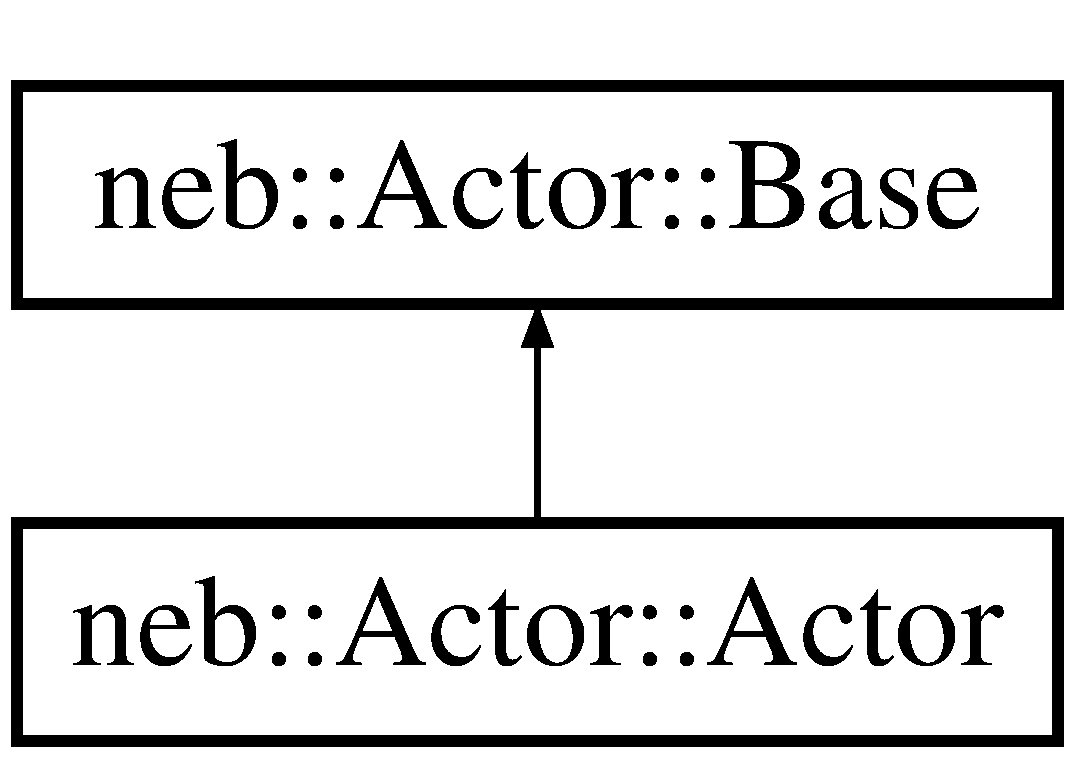
\includegraphics[height=5.000000cm]{classneb_1_1Actor_1_1Actor}
\end{center}
\end{figure}
\subsection*{\-Public \-Member \-Functions}
\begin{DoxyCompactItemize}
\item 
\hypertarget{classneb_1_1Actor_1_1Actor_aa4c6abb833d63779d289da4ca68ab74c}{{\bfseries \-Actor} (glutpp\-::actor\-::parent\-\_\-s)}\label{classneb_1_1Actor_1_1Actor_aa4c6abb833d63779d289da4ca68ab74c}

\item 
\hypertarget{classneb_1_1Actor_1_1Actor_a43fc6ba013fc4f53869e2779c336e0b8}{virtual void {\bfseries init} (glutpp\-::actor\-::desc\-\_\-s)}\label{classneb_1_1Actor_1_1Actor_a43fc6ba013fc4f53869e2779c336e0b8}

\item 
\hypertarget{classneb_1_1Actor_1_1Actor_a08ef274c9f457c294d7cdec495370834}{virtual void {\bfseries release} ()}\label{classneb_1_1Actor_1_1Actor_a08ef274c9f457c294d7cdec495370834}

\item 
\hypertarget{classneb_1_1Actor_1_1Actor_a08b8ce4f4dd32f0960c930f1774251d8}{virtual void {\bfseries add\-\_\-force} (double)}\label{classneb_1_1Actor_1_1Actor_a08b8ce4f4dd32f0960c930f1774251d8}

\item 
\hypertarget{classneb_1_1Actor_1_1Actor_a3199b630839ecbb3c67c350c0973919e}{virtual void {\bfseries set\-\_\-pose} (math\-::transform)}\label{classneb_1_1Actor_1_1Actor_a3199b630839ecbb3c67c350c0973919e}

\item 
\hypertarget{classneb_1_1Actor_1_1Actor_ad4d8742ef8b68bc252f38310d6c148cf}{virtual int {\bfseries fire} ()}\label{classneb_1_1Actor_1_1Actor_ad4d8742ef8b68bc252f38310d6c148cf}

\item 
\hypertarget{classneb_1_1Actor_1_1Actor_ac5c98f74c27c0ca570603fd53f44c34c}{virtual glutpp\-::actor\-::desc\-\_\-s {\bfseries get\-\_\-projectile} ()}\label{classneb_1_1Actor_1_1Actor_ac5c98f74c27c0ca570603fd53f44c34c}

\item 
\hypertarget{classneb_1_1Actor_1_1Actor_a0912b658a46c43bdf6c8cf05b41e9bd1}{virtual void {\bfseries create\-\_\-physics} ()}\label{classneb_1_1Actor_1_1Actor_a0912b658a46c43bdf6c8cf05b41e9bd1}

\item 
\hypertarget{classneb_1_1Actor_1_1Actor_a47a09288466f51d1f771b53ac74eec97}{virtual void {\bfseries init\-\_\-physics} ()}\label{classneb_1_1Actor_1_1Actor_a47a09288466f51d1f771b53ac74eec97}

\item 
\hypertarget{classneb_1_1Actor_1_1Actor_a04b545da670a47a37b152cfa3444767e}{virtual void {\bfseries step\-\_\-local} (double)}\label{classneb_1_1Actor_1_1Actor_a04b545da670a47a37b152cfa3444767e}

\item 
\hypertarget{classneb_1_1Actor_1_1Actor_a14f9a1b3e60bdad6ae4dfafd6f9580e8}{virtual void {\bfseries step\-\_\-remote} (double)}\label{classneb_1_1Actor_1_1Actor_a14f9a1b3e60bdad6ae4dfafd6f9580e8}

\item 
\hypertarget{classneb_1_1Actor_1_1Actor_ac1c1c4f015ed704b306d3aaa3fa3efc1}{virtual void {\bfseries print\-\_\-info} ()}\label{classneb_1_1Actor_1_1Actor_ac1c1c4f015ed704b306d3aaa3fa3efc1}

\end{DoxyCompactItemize}
\subsection*{\-Public \-Attributes}
\begin{DoxyCompactItemize}
\item 
\hypertarget{classneb_1_1Actor_1_1Actor_a4b5d6b98af98afece2a7f09c1ba7e69c}{physx\-::\-Px\-Actor $\ast$ {\bfseries px\-\_\-actor\-\_\-}}\label{classneb_1_1Actor_1_1Actor_a4b5d6b98af98afece2a7f09c1ba7e69c}

\end{DoxyCompactItemize}


\-The documentation for this class was generated from the following files\-:\begin{DoxyCompactItemize}
\item 
src/nebula/actor/\-Actor.\-hpp\item 
src/nebula/actor/\-Actor.\-cpp\end{DoxyCompactItemize}

\hypertarget{classneb_1_1Timer_1_1Actor}{\section{neb\-:\-:\-Timer\-:\-:\-Actor \-Class \-Reference}
\label{classneb_1_1Timer_1_1Actor}\index{neb\-::\-Timer\-::\-Actor@{neb\-::\-Timer\-::\-Actor}}
}
\subsection*{\-Public \-Types}
\begin{DoxyCompactItemize}
\item 
enum {\bfseries \-Type} \{ {\bfseries \-N\-O\-N\-E} =  0, 
{\bfseries \-R\-E\-L\-E\-A\-S\-E}
 \}
\end{DoxyCompactItemize}
\subsection*{\-Public \-Member \-Functions}
\begin{DoxyCompactItemize}
\item 
\hypertarget{classneb_1_1Timer_1_1Actor_ad187da5a4b8907ff074d331d85cf6aec}{{\bfseries \-Actor} (neb\-::\-Actor\-::\-Base\-\_\-s, neb\-::\-Timer\-::\-Actor\-::\-Type, double)}\label{classneb_1_1Timer_1_1Actor_ad187da5a4b8907ff074d331d85cf6aec}

\item 
\hypertarget{classneb_1_1Timer_1_1Actor_a8566283cef213c978a0d2b4a458b5a0a}{void {\bfseries activate} ()}\label{classneb_1_1Timer_1_1Actor_a8566283cef213c978a0d2b4a458b5a0a}

\end{DoxyCompactItemize}
\subsection*{\-Public \-Attributes}
\begin{DoxyCompactItemize}
\item 
\hypertarget{classneb_1_1Timer_1_1Actor_ab10e4bb47a25ad49687935b9fb0257de}{neb\-::\-Timer\-::\-Actor\-::\-Type {\bfseries type\-\_\-}}\label{classneb_1_1Timer_1_1Actor_ab10e4bb47a25ad49687935b9fb0257de}

\item 
\hypertarget{classneb_1_1Timer_1_1Actor_a359f5b4e9d2129521d65aeaed1c22cd3}{neb\-::\-Actor\-::\-Base\-\_\-w {\bfseries actor\-\_\-}}\label{classneb_1_1Timer_1_1Actor_a359f5b4e9d2129521d65aeaed1c22cd3}

\end{DoxyCompactItemize}


\-The documentation for this class was generated from the following file\-:\begin{DoxyCompactItemize}
\item 
src/nebula/timer/actor.\-hpp\end{DoxyCompactItemize}

\hypertarget{classneb_1_1packet_1_1actor__release}{\section{neb\-:\-:packet\-:\-:actor\-\_\-release \-Class \-Reference}
\label{classneb_1_1packet_1_1actor__release}\index{neb\-::packet\-::actor\-\_\-release@{neb\-::packet\-::actor\-\_\-release}}
}
\subsection*{\-Public \-Types}
\begin{DoxyCompactItemize}
\item 
\hypertarget{classneb_1_1packet_1_1actor__release_a00cd43364472a514dd494ff623b38435}{typedef std\-::shared\-\_\-ptr\*
$<$ \hyperlink{classgal_1_1network_1_1message}{gal\-::network\-::message} $>$ {\bfseries msg\-\_\-t}}\label{classneb_1_1packet_1_1actor__release_a00cd43364472a514dd494ff623b38435}

\end{DoxyCompactItemize}
\subsection*{\-Public \-Member \-Functions}
\begin{DoxyCompactItemize}
\item 
\hypertarget{classneb_1_1packet_1_1actor__release_a427941df801ea77f69c914b2cc15519e}{{\bfseries actor\-\_\-release} (int)}\label{classneb_1_1packet_1_1actor__release_a427941df801ea77f69c914b2cc15519e}

\item 
\hypertarget{classneb_1_1packet_1_1actor__release_ae798345bb4f2a39ebaba785036d1da89}{msg\-\_\-t {\bfseries serialize} ()}\label{classneb_1_1packet_1_1actor__release_ae798345bb4f2a39ebaba785036d1da89}

\item 
\hypertarget{classneb_1_1packet_1_1actor__release_a4ac4e4dd9da7391390d84e3549a590ff}{void {\bfseries write} (char $\ast$\&)}\label{classneb_1_1packet_1_1actor__release_a4ac4e4dd9da7391390d84e3549a590ff}

\item 
\hypertarget{classneb_1_1packet_1_1actor__release_a510a1b4586257e3bd25766e2f29f4239}{void {\bfseries read} (char $\ast$\&)}\label{classneb_1_1packet_1_1actor__release_a510a1b4586257e3bd25766e2f29f4239}

\item 
\hypertarget{classneb_1_1packet_1_1actor__release_a8068e8fa32dc9e51670dcea7e20ef8d6}{size\-\_\-t {\bfseries size} ()}\label{classneb_1_1packet_1_1actor__release_a8068e8fa32dc9e51670dcea7e20ef8d6}

\end{DoxyCompactItemize}
\subsection*{\-Public \-Attributes}
\begin{DoxyCompactItemize}
\item 
\hypertarget{classneb_1_1packet_1_1actor__release_a93c67e65fd2391fa5788ea4df62dea83}{int {\bfseries scene\-\_\-i\-\_\-}}\label{classneb_1_1packet_1_1actor__release_a93c67e65fd2391fa5788ea4df62dea83}

\item 
\hypertarget{classneb_1_1packet_1_1actor__release_adb41a9a1ca585fc92c5811a086088fba}{int {\bfseries actor\-\_\-size\-\_\-}}\label{classneb_1_1packet_1_1actor__release_adb41a9a1ca585fc92c5811a086088fba}

\item 
\hypertarget{classneb_1_1packet_1_1actor__release_a38a61811df9631de91ded02972d2e23b}{std\-::vector$<$ int $>$ {\bfseries actor\-\_\-i\-\_\-}}\label{classneb_1_1packet_1_1actor__release_a38a61811df9631de91ded02972d2e23b}

\end{DoxyCompactItemize}


\-The documentation for this class was generated from the following file\-:\begin{DoxyCompactItemize}
\item 
src/\-Nebula/network2/actor\-\_\-release.\-hh\end{DoxyCompactItemize}

\hypertarget{classneb_1_1app}{\section{neb\-:\-:app \-Class \-Reference}
\label{classneb_1_1app}\index{neb\-::app@{neb\-::app}}
}
\subsection*{\-Classes}
\begin{DoxyCompactItemize}
\item 
struct \hyperlink{structneb_1_1app_1_1flag}{flag}
\end{DoxyCompactItemize}
\subsection*{\-Public \-Member \-Functions}
\begin{DoxyCompactItemize}
\item 
\hypertarget{classneb_1_1app_a32164de189f14d814cfaca3e898b3a7f}{void {\bfseries init} ()}\label{classneb_1_1app_a32164de189f14d814cfaca3e898b3a7f}

\item 
\hypertarget{classneb_1_1app_a2e979ae56ad4a9f142816cf4df688907}{glutpp\-::window\-::window\-\_\-s {\bfseries create\-\_\-window} (int, int, int, int, char const $\ast$)}\label{classneb_1_1app_a2e979ae56ad4a9f142816cf4df688907}

\item 
\hypertarget{classneb_1_1app_abb769464af634e2ba8328437e23514f5}{neb\-::scene\-::scene\-\_\-s {\bfseries load\-\_\-scene\-\_\-local} (glutpp\-::scene\-::desc\-\_\-s)}\label{classneb_1_1app_abb769464af634e2ba8328437e23514f5}

\item 
\hypertarget{classneb_1_1app_a22d8080f269d8980d46eac3c2ce7c506}{neb\-::scene\-::scene\-\_\-s {\bfseries load\-\_\-scene\-\_\-remote} (glutpp\-::scene\-::desc\-\_\-s)}\label{classneb_1_1app_a22d8080f269d8980d46eac3c2ce7c506}

\item 
\hypertarget{classneb_1_1app_ad0e771e82f86ee786e1b342c18975fd2}{void {\bfseries load\-\_\-layout} (int, char const $\ast$)}\label{classneb_1_1app_ad0e771e82f86ee786e1b342c18975fd2}

\item 
\hypertarget{classneb_1_1app_ae364bf8705edcd0b65375d6831df326f}{int {\bfseries step} (double)}\label{classneb_1_1app_ae364bf8705edcd0b65375d6831df326f}

\item 
\hypertarget{classneb_1_1app_a3d1e3aa10f78a8e737352a90c1ff2004}{int {\bfseries loop} ()}\label{classneb_1_1app_a3d1e3aa10f78a8e737352a90c1ff2004}

\item 
\hypertarget{classneb_1_1app_a9e1237d528a0bfd338526751bff4a60d}{glutpp\-::window\-::window\-\_\-s {\bfseries get\-\_\-window} (int)}\label{classneb_1_1app_a9e1237d528a0bfd338526751bff4a60d}

\item 
\hypertarget{classneb_1_1app_a862cf4660c0ea97c1097414e2797e73f}{neb\-::scene\-::scene\-\_\-s {\bfseries get\-\_\-scene} (int)}\label{classneb_1_1app_a862cf4660c0ea97c1097414e2797e73f}

\item 
\hypertarget{classneb_1_1app_af87093d040035ac5d0d85dc5b11e0c0a}{neb\-::scene\-::scene\-\_\-s {\bfseries get\-\_\-scene} (glutpp\-::scene\-::addr\-\_\-s)}\label{classneb_1_1app_af87093d040035ac5d0d85dc5b11e0c0a}

\item 
\hypertarget{classneb_1_1app_acd137ce9a84bac35958d05c9d31ce113}{neb\-::\-Actor\-::\-Base\-\_\-s {\bfseries get\-\_\-actor} (glutpp\-::actor\-::addr\-\_\-s)}\label{classneb_1_1app_acd137ce9a84bac35958d05c9d31ce113}

\item 
\hypertarget{classneb_1_1app_a585d3455638323086057befeb4e91a1b}{void {\bfseries set\-\_\-should\-\_\-release} ()}\label{classneb_1_1app_a585d3455638323086057befeb4e91a1b}

\item 
\hypertarget{classneb_1_1app_aa558ff3c281cd6f6b7bdca7f5a7807ff}{int {\bfseries activate\-\_\-scene} (int, int)}\label{classneb_1_1app_aa558ff3c281cd6f6b7bdca7f5a7807ff}

\item 
\hypertarget{classneb_1_1app_a54affa2aa2f29724e15dee3fb4f01b2b}{int {\bfseries deactivate\-\_\-scene} (int)}\label{classneb_1_1app_a54affa2aa2f29724e15dee3fb4f01b2b}

\item 
\hypertarget{classneb_1_1app_a421f2d98f0857f6d73824740019c94f1}{int {\bfseries activate\-\_\-layout} (int, int)}\label{classneb_1_1app_a421f2d98f0857f6d73824740019c94f1}

\item 
\hypertarget{classneb_1_1app_a5b5b9384258da420e426d15f7c0753f3}{int {\bfseries deactivate\-\_\-layout} (int)}\label{classneb_1_1app_a5b5b9384258da420e426d15f7c0753f3}

\item 
\hypertarget{classneb_1_1app_a88525d86c44907e36e534ffb5d8c9f04}{void {\bfseries reset\-\_\-server} (unsigned short)}\label{classneb_1_1app_a88525d86c44907e36e534ffb5d8c9f04}

\item 
\hypertarget{classneb_1_1app_a94908472755f4f20846a75a5368825cb}{void {\bfseries reset\-\_\-client} (char const $\ast$, unsigned short)}\label{classneb_1_1app_a94908472755f4f20846a75a5368825cb}

\item 
\hypertarget{classneb_1_1app_a8250d1d585de859af0ae8098db7ad011}{void {\bfseries send\-\_\-server} (gal\-::network\-::message\-\_\-s)}\label{classneb_1_1app_a8250d1d585de859af0ae8098db7ad011}

\item 
\hypertarget{classneb_1_1app_a197b5f2b57db91d1fe622a9f40c65e15}{void {\bfseries send\-\_\-client} (gal\-::network\-::message\-\_\-s)}\label{classneb_1_1app_a197b5f2b57db91d1fe622a9f40c65e15}

\item 
\hypertarget{classneb_1_1app_a0ae9f3e3853e68b57b8ab76961151e7d}{int {\bfseries transmit\-\_\-scenes} (std\-::shared\-\_\-ptr$<$ \hyperlink{classneb_1_1network_1_1communicating}{neb\-::network\-::communicating} $>$)}\label{classneb_1_1app_a0ae9f3e3853e68b57b8ab76961151e7d}

\item 
\hypertarget{classneb_1_1app_a7a65b1cb131fba86458aa24964ad5170}{void {\bfseries recv\-\_\-scene\-\_\-create} (gal\-::network\-::message\-\_\-s)}\label{classneb_1_1app_a7a65b1cb131fba86458aa24964ad5170}

\item 
\hypertarget{classneb_1_1app_aa611d54b259485a21407eae7f71c9fde}{void {\bfseries recv\-\_\-actor\-\_\-create} (gal\-::network\-::message\-\_\-s)}\label{classneb_1_1app_aa611d54b259485a21407eae7f71c9fde}

\item 
\hypertarget{classneb_1_1app_adbaa519543d2e061c269b216b5c72ada}{void {\bfseries recv\-\_\-actor\-\_\-update} (gal\-::network\-::message\-\_\-s)}\label{classneb_1_1app_adbaa519543d2e061c269b216b5c72ada}

\item 
\hypertarget{classneb_1_1app_ad449a2212662a30fcc02f4677e535b77}{void {\bfseries recv\-\_\-actor\-\_\-event} (gal\-::network\-::message\-\_\-s)}\label{classneb_1_1app_ad449a2212662a30fcc02f4677e535b77}

\item 
\hypertarget{classneb_1_1app_aa4856f8e8eb8ccd5914689d6451f64e4}{void {\bfseries recv\-\_\-control\-\_\-create} (gal\-::network\-::message\-\_\-s)}\label{classneb_1_1app_aa4856f8e8eb8ccd5914689d6451f64e4}

\item 
\hypertarget{classneb_1_1app_a7e6cb986c8b71ed1a2e2b5116ea4d54d}{void {\bfseries recv\-\_\-control\-\_\-update} (gal\-::network\-::message\-\_\-s)}\label{classneb_1_1app_a7e6cb986c8b71ed1a2e2b5116ea4d54d}

\item 
\hypertarget{classneb_1_1app_a878745ce448b6a32639f9b28c91d3dac}{void {\bfseries f} (unsigned int)}\label{classneb_1_1app_a878745ce448b6a32639f9b28c91d3dac}

\item 
\hypertarget{classneb_1_1app_a4158adddede1a017c151da072503dcad}{unsigned int {\bfseries f} ()}\label{classneb_1_1app_a4158adddede1a017c151da072503dcad}

\end{DoxyCompactItemize}
\subsection*{\-Public \-Attributes}
\begin{DoxyCompactItemize}
\item 
\hypertarget{classneb_1_1app_a541f268dba5963578a9a7985db8ab465}{unsigned int {\bfseries flag\-\_\-}}\label{classneb_1_1app_a541f268dba5963578a9a7985db8ab465}

\item 
\hypertarget{classneb_1_1app_ad6b61ebea17df0281aa2f9e0caa7f675}{gal\-::map$<$ glutpp\-::window\-::window $>$ {\bfseries windows\-\_\-}}\label{classneb_1_1app_ad6b61ebea17df0281aa2f9e0caa7f675}

\item 
\hypertarget{classneb_1_1app_a5e83d509c862b9050e3840a7fe15ac01}{gal\-::map$<$ glutpp\-::gui\-::layout $>$ {\bfseries layouts\-\_\-}}\label{classneb_1_1app_a5e83d509c862b9050e3840a7fe15ac01}

\item 
\hypertarget{classneb_1_1app_ac53edb0e3764d01881d544bf27106a89}{gal\-::map$<$ \hyperlink{classneb_1_1scene_1_1scene}{neb\-::scene\-::scene} $>$ {\bfseries scenes\-\_\-}}\label{classneb_1_1app_ac53edb0e3764d01881d544bf27106a89}

\item 
\hypertarget{classneb_1_1app_a23c6f2ed724892216392a4607606f9ed}{gal\-::timer\-::timer\-\_\-set {\bfseries timer\-\_\-set\-\_\-}}\label{classneb_1_1app_a23c6f2ed724892216392a4607606f9ed}

\end{DoxyCompactItemize}


\-The documentation for this class was generated from the following files\-:\begin{DoxyCompactItemize}
\item 
src/nebula/app.\-hpp\item 
src/nebula/app.\-cpp\end{DoxyCompactItemize}

\hypertarget{classneb_1_1Actor_1_1Base}{\section{neb\-:\-:\-Actor\-:\-:\-Base \-Class \-Reference}
\label{classneb_1_1Actor_1_1Base}\index{neb\-::\-Actor\-::\-Base@{neb\-::\-Actor\-::\-Base}}
}


\-Base  




{\ttfamily \#include $<$\-Base.\-hpp$>$}

\-Inheritance diagram for neb\-:\-:\-Actor\-:\-:\-Base\-:\begin{figure}[H]
\begin{center}
\leavevmode
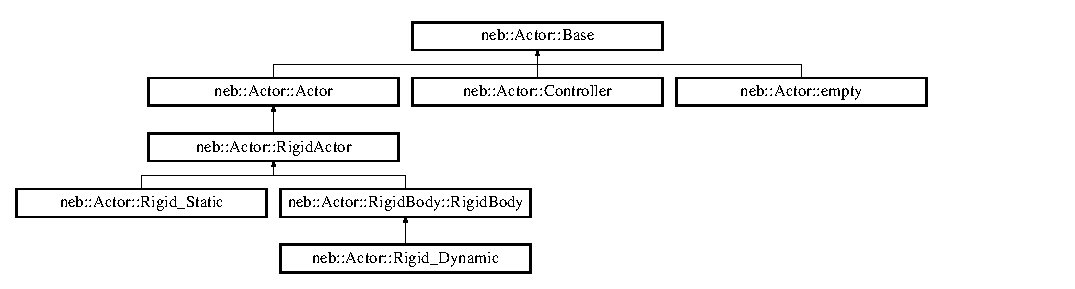
\includegraphics[height=3.431373cm]{classneb_1_1Actor_1_1Base}
\end{center}
\end{figure}
\subsection*{\-Public \-Member \-Functions}
\begin{DoxyCompactItemize}
\item 
\hypertarget{classneb_1_1Actor_1_1Base_a2476f443f7d6b8c60b3912953eec0842}{{\bfseries \-Base} (glutpp\-::actor\-::parent\-\_\-s)}\label{classneb_1_1Actor_1_1Base_a2476f443f7d6b8c60b3912953eec0842}

\item 
\hypertarget{classneb_1_1Actor_1_1Base_a972bd459843929bd090f093d215d540b}{virtual void {\bfseries init} (glutpp\-::actor\-::desc\-\_\-s)}\label{classneb_1_1Actor_1_1Base_a972bd459843929bd090f093d215d540b}

\item 
\hypertarget{classneb_1_1Actor_1_1Base_aee25af3cd56f3aec8a3e2db274bb0d1d}{virtual void {\bfseries release} ()}\label{classneb_1_1Actor_1_1Base_aee25af3cd56f3aec8a3e2db274bb0d1d}

\item 
\hypertarget{classneb_1_1Actor_1_1Base_a2f335051e5a6f833cad94da551bf9f82}{neb\-::\-Actor\-::\-Base\-\_\-s {\bfseries create\-\_\-actor\-\_\-local} (glutpp\-::actor\-::desc\-\_\-s)}\label{classneb_1_1Actor_1_1Base_a2f335051e5a6f833cad94da551bf9f82}

\item 
\hypertarget{classneb_1_1Actor_1_1Base_a045e31459829bbbb5a49dccf0e7d9b67}{neb\-::\-Actor\-::\-Base\-\_\-s {\bfseries create\-\_\-actor\-\_\-remote} (glutpp\-::actor\-::addr\-\_\-s, glutpp\-::actor\-::desc\-\_\-s)}\label{classneb_1_1Actor_1_1Base_a045e31459829bbbb5a49dccf0e7d9b67}

\item 
\hypertarget{classneb_1_1Actor_1_1Base_ae60a17296d6a2393c7662340673073a6}{void {\bfseries create\-\_\-shapes} (glutpp\-::actor\-::desc\-\_\-s)}\label{classneb_1_1Actor_1_1Base_ae60a17296d6a2393c7662340673073a6}

\item 
\hypertarget{classneb_1_1Actor_1_1Base_a1c6cb73654d5f395c86de63be1f25d1c}{void {\bfseries create\-\_\-children} (glutpp\-::actor\-::desc\-\_\-s)}\label{classneb_1_1Actor_1_1Base_a1c6cb73654d5f395c86de63be1f25d1c}

\item 
\hypertarget{classneb_1_1Actor_1_1Base_a03d72471ba01b7c7df310e02173240e0}{virtual void {\bfseries create\-\_\-physics} ()}\label{classneb_1_1Actor_1_1Base_a03d72471ba01b7c7df310e02173240e0}

\item 
\hypertarget{classneb_1_1Actor_1_1Base_a731bb18d1c9ea82bffbb2a21142bdd27}{virtual void {\bfseries init\-\_\-physics} ()}\label{classneb_1_1Actor_1_1Base_a731bb18d1c9ea82bffbb2a21142bdd27}

\item 
\hypertarget{classneb_1_1Actor_1_1Base_ae3983e94b6e4311f9830fb257bdd430b}{neb\-::app\-\_\-s {\bfseries get\-\_\-app} ()}\label{classneb_1_1Actor_1_1Base_ae3983e94b6e4311f9830fb257bdd430b}

\item 
\hypertarget{classneb_1_1Actor_1_1Base_a9ecd15cc92581b224343e345533ceda8}{neb\-::scene\-::scene\-\_\-s {\bfseries get\-\_\-scene} ()}\label{classneb_1_1Actor_1_1Base_a9ecd15cc92581b224343e345533ceda8}

\item 
\hypertarget{classneb_1_1Actor_1_1Base_af8d94037bac4bbef8205cb491ed8f6f6}{neb\-::\-Actor\-::\-Base\-\_\-s {\bfseries get\-\_\-actor} (int)}\label{classneb_1_1Actor_1_1Base_af8d94037bac4bbef8205cb491ed8f6f6}

\item 
neb\-::\-Actor\-::\-Base\-\_\-s \hyperlink{classneb_1_1Actor_1_1Base_a0e31f35ba460d472e9730d1e9e53933d}{get\-\_\-actor} (glutpp\-::actor\-::addr\-\_\-s addr)
\begin{DoxyCompactList}\small\item\em get child actor \end{DoxyCompactList}\item 
\hypertarget{classneb_1_1Actor_1_1Base_a6aea29e7c87c3bb8507d2e249fe18a9b}{virtual glutpp\-::actor\-::desc\-\_\-s {\bfseries get\-\_\-projectile} ()}\label{classneb_1_1Actor_1_1Base_a6aea29e7c87c3bb8507d2e249fe18a9b}

\item 
\hypertarget{classneb_1_1Actor_1_1Base_a83a135f3543d02c0bd8a6d32b6d1d386}{virtual void {\bfseries hit} ()}\label{classneb_1_1Actor_1_1Base_a83a135f3543d02c0bd8a6d32b6d1d386}

\item 
\hypertarget{classneb_1_1Actor_1_1Base_a4c2e2a30b3e7c801e9e4e04552e10b30}{virtual void {\bfseries damage} (float)}\label{classneb_1_1Actor_1_1Base_a4c2e2a30b3e7c801e9e4e04552e10b30}

\item 
\hypertarget{classneb_1_1Actor_1_1Base_af57cfb2160c8263244a2ee0bd9b4b254}{virtual void {\bfseries step\-\_\-local} (double)}\label{classneb_1_1Actor_1_1Base_af57cfb2160c8263244a2ee0bd9b4b254}

\item 
\hypertarget{classneb_1_1Actor_1_1Base_af82f96cdf3dd4c63a61d870a87ce06e1}{virtual void {\bfseries step\-\_\-remote} (double)}\label{classneb_1_1Actor_1_1Base_af82f96cdf3dd4c63a61d870a87ce06e1}

\item 
\hypertarget{classneb_1_1Actor_1_1Base_a677f636fb8e89f78f5c73c54387da08b}{neb\-::\-Actor\-::raw\-\_\-s {\bfseries get\-\_\-raw\-\_\-base} ()}\label{classneb_1_1Actor_1_1Base_a677f636fb8e89f78f5c73c54387da08b}

\item 
\hypertarget{classneb_1_1Actor_1_1Base_a514f9cacb1d0029e7a98e7ff7608fac3}{void {\bfseries connect} (glutpp\-::window\-::window\-\_\-s)}\label{classneb_1_1Actor_1_1Base_a514f9cacb1d0029e7a98e7ff7608fac3}

\item 
\hypertarget{classneb_1_1Actor_1_1Base_a3e4da379542de484eb1f748da335e957}{int {\bfseries key\-\_\-fun} (int, int, int, int)}\label{classneb_1_1Actor_1_1Base_a3e4da379542de484eb1f748da335e957}

\item 
\hypertarget{classneb_1_1Actor_1_1Base_ac903d214c5db5e8636af190993481e46}{virtual int {\bfseries fire} ()}\label{classneb_1_1Actor_1_1Base_ac903d214c5db5e8636af190993481e46}

\end{DoxyCompactItemize}
\begin{Indent}{\bf \-Convertion}\par
\begin{DoxyCompactItemize}
\item 
\hypertarget{classneb_1_1Actor_1_1Base_ae490845b7ff5339167c63305eefb0c1d}{\-Base\-\_\-s {\bfseries is\-Base} ()}\label{classneb_1_1Actor_1_1Base_ae490845b7ff5339167c63305eefb0c1d}

\item 
\hypertarget{classneb_1_1Actor_1_1Base_a71e76e4c849cc89220c3b3bb78a147b0}{\-Rigid\-Actor\-\_\-s {\bfseries is\-Rigid\-Actor} ()}\label{classneb_1_1Actor_1_1Base_a71e76e4c849cc89220c3b3bb78a147b0}

\item 
\hypertarget{classneb_1_1Actor_1_1Base_aceb861c27923ebcaff572d59d0155ef8}{rigid\-\_\-body\-::rigid\-\_\-body\-\_\-s {\bfseries is\-Rigid\-Body} ()}\label{classneb_1_1Actor_1_1Base_aceb861c27923ebcaff572d59d0155ef8}

\end{DoxyCompactItemize}
\end{Indent}
\subsection*{\-Public \-Attributes}
\begin{DoxyCompactItemize}
\item 
\hypertarget{classneb_1_1Actor_1_1Base_a21de3294925b6c5a2eecad868920f52f}{glutpp\-::actor\-::mode\-\_\-update\-::e {\bfseries mode\-\_\-update\-\_\-}}\label{classneb_1_1Actor_1_1Base_a21de3294925b6c5a2eecad868920f52f}

\item 
\hypertarget{classneb_1_1Actor_1_1Base_acb77fc381cc60940a1f73605a006b7f5}{glutpp\-::window\-::window\-\_\-w {\bfseries window\-\_\-}}\label{classneb_1_1Actor_1_1Base_acb77fc381cc60940a1f73605a006b7f5}

\item 
\hypertarget{classneb_1_1Actor_1_1Base_ae29c1200bb17c5372d99813ed28822c5}{\begin{tabbing}
xx\=xx\=xx\=xx\=xx\=xx\=xx\=xx\=xx\=\kill
struct \{\\
\>key\_fun\_c {\bfseries key\_fun\_}\\
\} {\bfseries conn\_}}\label{classneb_1_1Actor_1_1Base_ae29c1200bb17c5372d99813ed28822c5}
\\

\end{tabbing}\end{DoxyCompactItemize}


\subsection{\-Detailed \-Description}
\-Base 

\subsection{\-Member \-Function \-Documentation}
\hypertarget{classneb_1_1Actor_1_1Base_a0e31f35ba460d472e9730d1e9e53933d}{\index{neb\-::\-Actor\-::\-Base@{neb\-::\-Actor\-::\-Base}!get\-\_\-actor@{get\-\_\-actor}}
\index{get\-\_\-actor@{get\-\_\-actor}!neb::Actor::Base@{neb\-::\-Actor\-::\-Base}}
\subsubsection[{get\-\_\-actor}]{\setlength{\rightskip}{0pt plus 5cm}neb\-::actor\-::\-Base\-\_\-s neb\-::actor\-::\-Base\-::get\-\_\-actor (
\begin{DoxyParamCaption}
\item[{glutpp\-::actor\-::addr\-\_\-s}]{addr}
\end{DoxyParamCaption}
)}}\label{classneb_1_1Actor_1_1Base_a0e31f35ba460d472e9730d1e9e53933d}


get child actor 

casts gru actor to nebula actor 
\begin{DoxyParams}{\-Parameters}
{\em addr} & address of actor \\
\hline
\end{DoxyParams}


\-The documentation for this class was generated from the following files\-:\begin{DoxyCompactItemize}
\item 
src/nebula/actor/\-Base.\-hpp\item 
src/nebula/actor/\-Base.\-cpp\end{DoxyCompactItemize}

\hypertarget{classneb_1_1box}{
\section{neb::box Class Reference}
\label{classneb_1_1box}\index{neb::box@{neb::box}}
}
\subsection*{Public Attributes}
\begin{DoxyCompactItemize}
\item 
\hypertarget{classneb_1_1box_a7c1a37ac522ae516df9e6058a756c7d3}{
math::vec3 {\bfseries s\_\-}}
\label{classneb_1_1box_a7c1a37ac522ae516df9e6058a756c7d3}

\end{DoxyCompactItemize}


The documentation for this class was generated from the following file:\begin{DoxyCompactItemize}
\item 
src/nebula/actor/geometry.hpp\end{DoxyCompactItemize}

\hypertarget{classneb_1_1network_1_1client}{
\section{neb::network::client Class Reference}
\label{classneb_1_1network_1_1client}\index{neb::network::client@{neb::network::client}}
}
Inheritance diagram for neb::network::client::\begin{figure}[H]
\begin{center}
\leavevmode
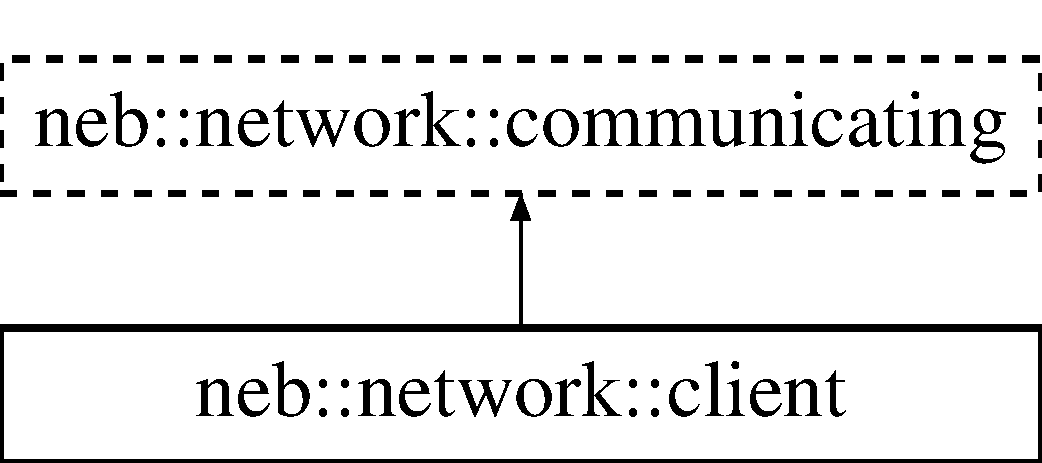
\includegraphics[height=2cm]{classneb_1_1network_1_1client}
\end{center}
\end{figure}
\subsection*{Public Member Functions}
\begin{DoxyCompactItemize}
\item 
\hypertarget{classneb_1_1network_1_1client_a4f117f86f1d548c492645b47ca3b1fb0}{
{\bfseries client} (neb::app\_\-s, char const $\ast$, unsigned short)}
\label{classneb_1_1network_1_1client_a4f117f86f1d548c492645b47ca3b1fb0}

\item 
\hypertarget{classneb_1_1network_1_1client_a04d1cdc645678b66a0c0bdfcf9eb3c1d}{
void {\bfseries process} (gal::network::message::shared\_\-t)}
\label{classneb_1_1network_1_1client_a04d1cdc645678b66a0c0bdfcf9eb3c1d}

\end{DoxyCompactItemize}


The documentation for this class was generated from the following files:\begin{DoxyCompactItemize}
\item 
src/nebula/network/client.hpp\item 
src/nebula/network/client.cpp\end{DoxyCompactItemize}

\hypertarget{classneb_1_1network_1_1communicating}{
\section{neb::network::communicating Class Reference}
\label{classneb_1_1network_1_1communicating}\index{neb::network::communicating@{neb::network::communicating}}
}
Inheritance diagram for neb::network::communicating::\begin{figure}[H]
\begin{center}
\leavevmode
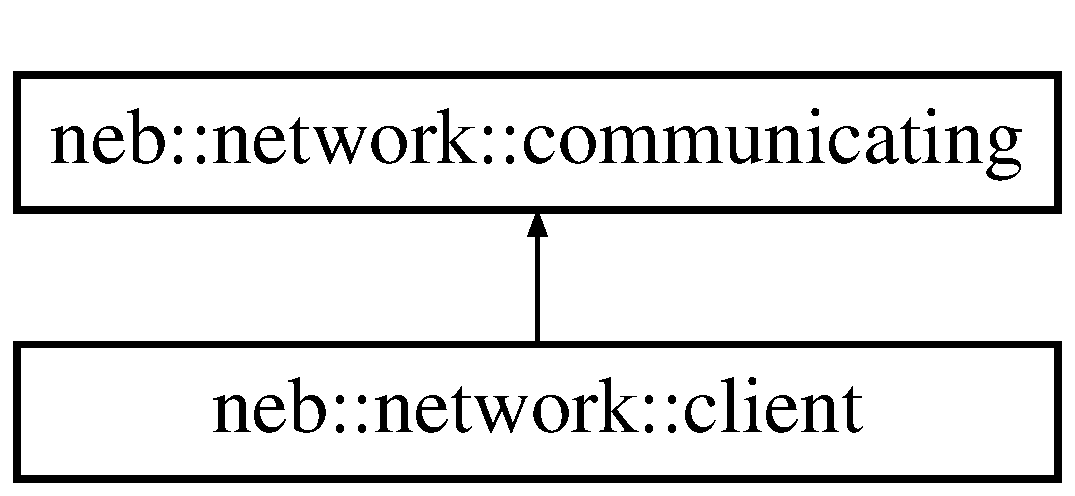
\includegraphics[height=2cm]{classneb_1_1network_1_1communicating}
\end{center}
\end{figure}
\subsection*{Public Member Functions}
\begin{DoxyCompactItemize}
\item 
\hypertarget{classneb_1_1network_1_1communicating_aa56d7ee8b8546ecc25b2cc63603184e9}{
{\bfseries communicating} (neb::app\_\-s, int)}
\label{classneb_1_1network_1_1communicating_aa56d7ee8b8546ecc25b2cc63603184e9}

\item 
\hypertarget{classneb_1_1network_1_1communicating_a98c549330850584cd5ec57028785b777}{
void {\bfseries process} (gal::network::message::shared\_\-t)}
\label{classneb_1_1network_1_1communicating_a98c549330850584cd5ec57028785b777}

\end{DoxyCompactItemize}
\subsection*{Public Attributes}
\begin{DoxyCompactItemize}
\item 
\hypertarget{classneb_1_1network_1_1communicating_a9bac744763987c357b07a070ce2f1215}{
neb::app\_\-w {\bfseries app\_\-}}
\label{classneb_1_1network_1_1communicating_a9bac744763987c357b07a070ce2f1215}

\end{DoxyCompactItemize}


The documentation for this class was generated from the following files:\begin{DoxyCompactItemize}
\item 
src/nebula/network/communicating.hpp\item 
src/nebula/network/communicating.cpp\end{DoxyCompactItemize}

\hypertarget{classneb_1_1control_1_1rigid__body_1_1control}{
\section{neb::control::rigid\_\-body::control Class Reference}
\label{classneb_1_1control_1_1rigid__body_1_1control}\index{neb::control::rigid\_\-body::control@{neb::control::rigid\_\-body::control}}
}


Rigid Body An object (what did I mean by 'object' here, an actor?) makes no distinction between local and remote. In a remote scene, the actor will send a \hyperlink{classneb_1_1control_1_1rigid__body_1_1control}{control} update message. In a local scene, the actor will call upon stored values; it makes no difference to the actor whether these value were set by calls to key\_\-fun or by a \hyperlink{classneb_1_1control_1_1rigid__body_1_1control}{control} update message. This creates requirements for how \hyperlink{classneb_1_1control_1_1rigid__body_1_1control}{control} works. All infomation needed to determine force and torque at a given point in time must be stored in \hyperlink{classneb_1_1control_1_1rigid__body_1_1raw}{raw}.  


{\ttfamily \#include $<$control.hpp$>$}\subsection*{Public Member Functions}
\begin{DoxyCompactItemize}
\item 
\hypertarget{classneb_1_1control_1_1rigid__body_1_1control_a66fc3682afd8f4a94ccd241cb3ddddb3}{
virtual int {\bfseries key\_\-fun} (int, int, int, int)}
\label{classneb_1_1control_1_1rigid__body_1_1control_a66fc3682afd8f4a94ccd241cb3ddddb3}

\item 
\hypertarget{classneb_1_1control_1_1rigid__body_1_1control_a0649203ba08991125250be485dad9308}{
void {\bfseries step\_\-local} (double)}
\label{classneb_1_1control_1_1rigid__body_1_1control_a0649203ba08991125250be485dad9308}

\item 
\hypertarget{classneb_1_1control_1_1rigid__body_1_1control_a347b217d2133bf301aa9f31e084ccd6a}{
void {\bfseries step\_\-local0} (double)}
\label{classneb_1_1control_1_1rigid__body_1_1control_a347b217d2133bf301aa9f31e084ccd6a}

\item 
\hypertarget{classneb_1_1control_1_1rigid__body_1_1control_a6fad3693d3a31440201a928bc04e71d4}{
void {\bfseries step\_\-local1} (double)}
\label{classneb_1_1control_1_1rigid__body_1_1control_a6fad3693d3a31440201a928bc04e71d4}

\item 
\hypertarget{classneb_1_1control_1_1rigid__body_1_1control_aeaae8332076304e32a811e6f06410e18}{
math::vec3$<$ double $>$ {\bfseries f} ()}
\label{classneb_1_1control_1_1rigid__body_1_1control_aeaae8332076304e32a811e6f06410e18}

\item 
\hypertarget{classneb_1_1control_1_1rigid__body_1_1control_a0f2f5f0c00acbf26b2ae23c1db70f1d9}{
math::vec3$<$ double $>$ {\bfseries t} ()}
\label{classneb_1_1control_1_1rigid__body_1_1control_a0f2f5f0c00acbf26b2ae23c1db70f1d9}

\item 
\hypertarget{classneb_1_1control_1_1rigid__body_1_1control_a13cbe1e4aa9e9cbd38cc2424526779a3}{
void {\bfseries print} ()}
\label{classneb_1_1control_1_1rigid__body_1_1control_a13cbe1e4aa9e9cbd38cc2424526779a3}

\end{DoxyCompactItemize}
\subsection*{Public Attributes}
\begin{DoxyCompactItemize}
\item 
\hypertarget{classneb_1_1control_1_1rigid__body_1_1control_a5a8dc4754c9d46b288a468e0033af474}{
neb::actor::Base\_\-w {\bfseries actor\_\-}}
\label{classneb_1_1control_1_1rigid__body_1_1control_a5a8dc4754c9d46b288a468e0033af474}

\item 
\hypertarget{classneb_1_1control_1_1rigid__body_1_1control_a4a547bcc332479f91eecfcbaccfcb1c2}{
\hyperlink{classneb_1_1control_1_1rigid__body_1_1raw}{neb::control::rigid\_\-body::raw} {\bfseries raw\_\-}}
\label{classneb_1_1control_1_1rigid__body_1_1control_a4a547bcc332479f91eecfcbaccfcb1c2}

\item 
\hypertarget{classneb_1_1control_1_1rigid__body_1_1control_a5209e25d3b03696cd84710f34c991dea}{
\begin{tabbing}
xx\=xx\=xx\=xx\=xx\=xx\=xx\=xx\=xx\=\kill
struct \{\\
\>key\_fun\_c {\bfseries key\_fun\_}\\
\} {\bfseries conn\_}}
\label{classneb_1_1control_1_1rigid__body_1_1control_a5209e25d3b03696cd84710f34c991dea}
\\

\end{tabbing}\item 
\hypertarget{classneb_1_1control_1_1rigid__body_1_1control_a621b7abb234dfeae7db854a70899a96f}{
gal::control::control {\bfseries pid\_\-}}
\label{classneb_1_1control_1_1rigid__body_1_1control_a621b7abb234dfeae7db854a70899a96f}

\item 
\hypertarget{classneb_1_1control_1_1rigid__body_1_1control_a15a9bb7db7b5d2b8dc8d99a3bff00d68}{
double {\bfseries last\_\-}}
\label{classneb_1_1control_1_1rigid__body_1_1control_a15a9bb7db7b5d2b8dc8d99a3bff00d68}

\end{DoxyCompactItemize}


\subsection{Detailed Description}
Rigid Body An object (what did I mean by 'object' here, an actor?) makes no distinction between local and remote. In a remote scene, the actor will send a \hyperlink{classneb_1_1control_1_1rigid__body_1_1control}{control} update message. In a local scene, the actor will call upon stored values; it makes no difference to the actor whether these value were set by calls to key\_\-fun or by a \hyperlink{classneb_1_1control_1_1rigid__body_1_1control}{control} update message. This creates requirements for how \hyperlink{classneb_1_1control_1_1rigid__body_1_1control}{control} works. All infomation needed to determine force and torque at a given point in time must be stored in \hyperlink{classneb_1_1control_1_1rigid__body_1_1raw}{raw}. 

The documentation for this class was generated from the following files:\begin{DoxyCompactItemize}
\item 
src/nebula/control/rigid\_\-body/control.hpp\item 
src/nebula/control/rigid\_\-body/control.cpp\end{DoxyCompactItemize}

\hypertarget{classneb_1_1Actor_1_1Controller}{\section{neb\-:\-:\-Actor\-:\-:\-Controller \-Class \-Reference}
\label{classneb_1_1Actor_1_1Controller}\index{neb\-::\-Actor\-::\-Controller@{neb\-::\-Actor\-::\-Controller}}
}
\-Inheritance diagram for neb\-:\-:\-Actor\-:\-:\-Controller\-:\begin{figure}[H]
\begin{center}
\leavevmode
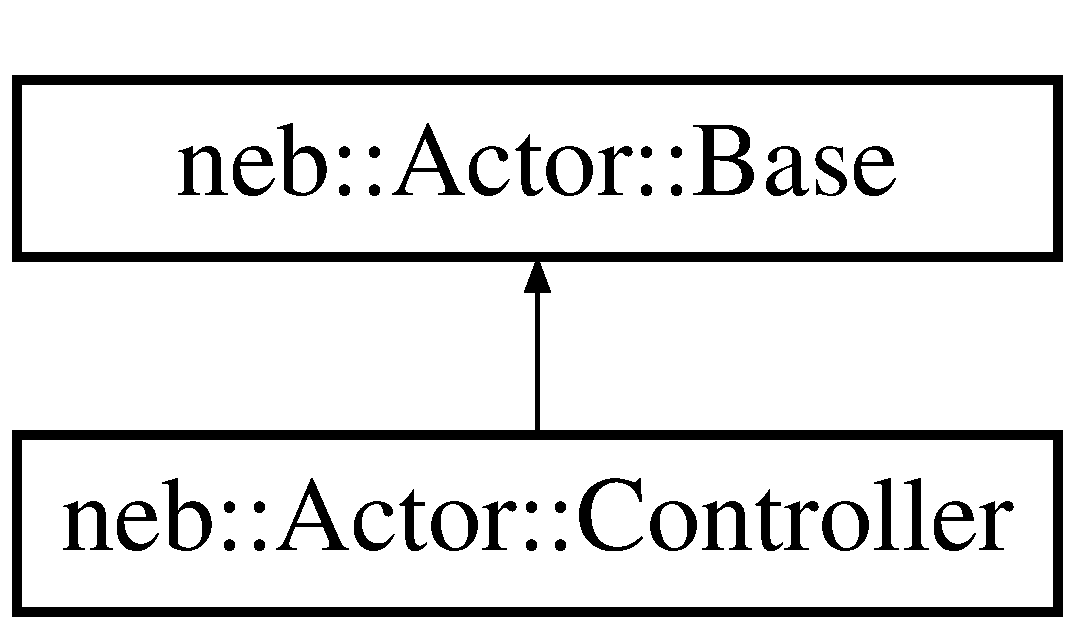
\includegraphics[height=2.000000cm]{classneb_1_1Actor_1_1Controller}
\end{center}
\end{figure}
\subsection*{\-Public \-Member \-Functions}
\begin{DoxyCompactItemize}
\item 
\hypertarget{classneb_1_1Actor_1_1Controller_aeedad5d671d8d4bc4398efd7be7fc005}{{\bfseries \-Controller} (glutpp\-::actor\-::parent\-\_\-s)}\label{classneb_1_1Actor_1_1Controller_aeedad5d671d8d4bc4398efd7be7fc005}

\item 
\hypertarget{classneb_1_1Actor_1_1Controller_ac6f5996da2aea174de794de4ffc647f4}{virtual void {\bfseries release} ()}\label{classneb_1_1Actor_1_1Controller_ac6f5996da2aea174de794de4ffc647f4}

\item 
\hypertarget{classneb_1_1Actor_1_1Controller_a95830d761987167e8ab122f3ca16346f}{virtual void {\bfseries step} (float)}\label{classneb_1_1Actor_1_1Controller_a95830d761987167e8ab122f3ca16346f}

\item 
\hypertarget{classneb_1_1Actor_1_1Controller_aad1420da60579f17c8dec8dad2a517bb}{virtual void {\bfseries init} (glutpp\-::actor\-::desc\-\_\-s)}\label{classneb_1_1Actor_1_1Controller_aad1420da60579f17c8dec8dad2a517bb}

\item 
\hypertarget{classneb_1_1Actor_1_1Controller_ab8ab78f513b014f112895de7dad43040}{virtual void {\bfseries add\-\_\-force} ()}\label{classneb_1_1Actor_1_1Controller_ab8ab78f513b014f112895de7dad43040}

\end{DoxyCompactItemize}
\subsection*{\-Public \-Attributes}
\begin{DoxyCompactItemize}
\item 
\hypertarget{classneb_1_1Actor_1_1Controller_aa692b62e071660a4e182406efb10272b}{physx\-::\-Px\-Controller $\ast$ {\bfseries px\-\_\-controller\-\_\-}}\label{classneb_1_1Actor_1_1Controller_aa692b62e071660a4e182406efb10272b}

\end{DoxyCompactItemize}


\-The documentation for this class was generated from the following files\-:\begin{DoxyCompactItemize}
\item 
src/nebula/actor/\-Controller.\-hpp\item 
src/nebula/actor/\-Controller.\-cpp\end{DoxyCompactItemize}

\hypertarget{classneb_1_1network_1_1control_1_1rigid__body_1_1create}{\section{neb\-:\-:network\-:\-:control\-:\-:rigid\-\_\-body\-:\-:create \-Class \-Reference}
\label{classneb_1_1network_1_1control_1_1rigid__body_1_1create}\index{neb\-::network\-::control\-::rigid\-\_\-body\-::create@{neb\-::network\-::control\-::rigid\-\_\-body\-::create}}
}
\subsection*{\-Public \-Member \-Functions}
\begin{DoxyCompactItemize}
\item 
\hypertarget{classneb_1_1network_1_1control_1_1rigid__body_1_1create_af3941f85f8c8499440492a4b4373231f}{glutpp\-::actor\-::addr\-\_\-s {\bfseries get\-\_\-addr} ()}\label{classneb_1_1network_1_1control_1_1rigid__body_1_1create_af3941f85f8c8499440492a4b4373231f}

\end{DoxyCompactItemize}


\-The documentation for this class was generated from the following file\-:\begin{DoxyCompactItemize}
\item 
src/nebula/network/message.\-hpp\end{DoxyCompactItemize}

\hypertarget{classDefaultErrorCallback}{\section{\-Default\-Error\-Callback \-Class \-Reference}
\label{classDefaultErrorCallback}\index{\-Default\-Error\-Callback@{\-Default\-Error\-Callback}}
}
\subsection*{\-Public \-Member \-Functions}
\begin{DoxyCompactItemize}
\item 
\hypertarget{classDefaultErrorCallback_ae95118f6a45b47a1b72af9417f80d84e}{void {\bfseries report\-Error} (physx\-::\-Px\-Error\-Code\-::\-Enum code, char const $\ast$message, char const $\ast$file, int line)}\label{classDefaultErrorCallback_ae95118f6a45b47a1b72af9417f80d84e}

\end{DoxyCompactItemize}


\-The documentation for this class was generated from the following files\-:\begin{DoxyCompactItemize}
\item 
src/nebula/physics.\-hpp\item 
src/nebula/physics.\-cpp\end{DoxyCompactItemize}

\hypertarget{classneb_1_1Actor_1_1empty}{\section{neb\-:\-:\-Actor\-:\-:empty \-Class \-Reference}
\label{classneb_1_1Actor_1_1empty}\index{neb\-::\-Actor\-::empty@{neb\-::\-Actor\-::empty}}
}
\-Inheritance diagram for neb\-:\-:\-Actor\-:\-:empty\-:\begin{figure}[H]
\begin{center}
\leavevmode
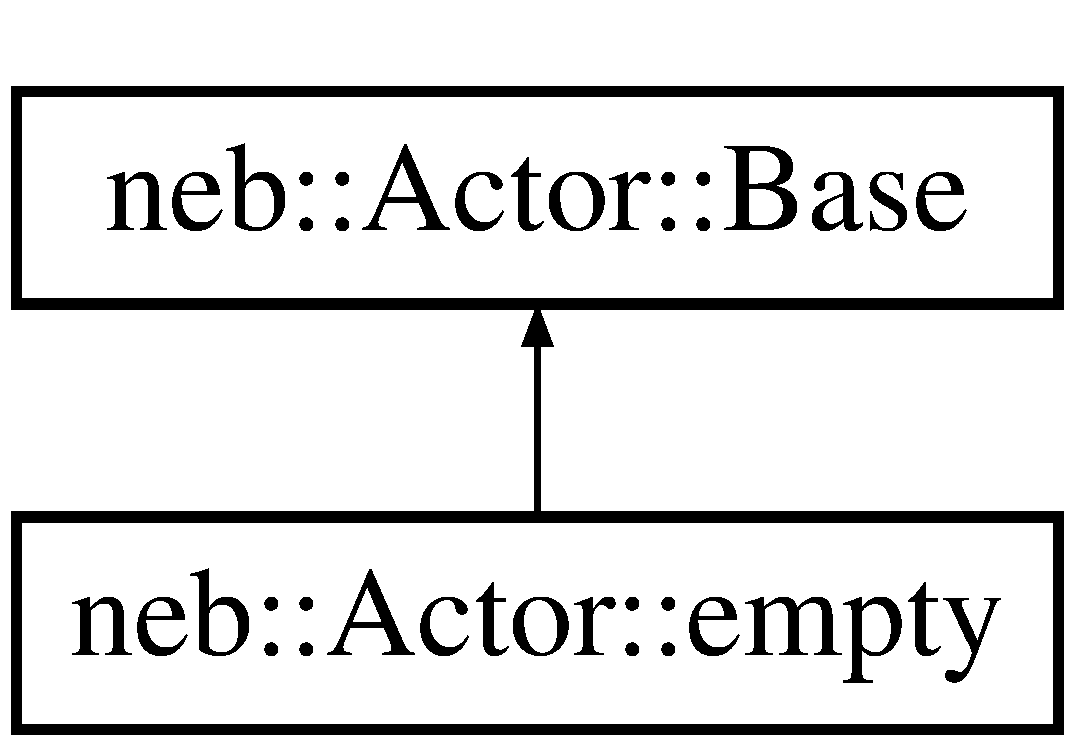
\includegraphics[height=2.000000cm]{classneb_1_1Actor_1_1empty}
\end{center}
\end{figure}
\subsection*{\-Public \-Member \-Functions}
\begin{DoxyCompactItemize}
\item 
\hypertarget{classneb_1_1Actor_1_1empty_a986bad0e65988e8561985a8500cc2bdb}{{\bfseries empty} (glutpp\-::actor\-::parent\-\_\-s)}\label{classneb_1_1Actor_1_1empty_a986bad0e65988e8561985a8500cc2bdb}

\item 
\hypertarget{classneb_1_1Actor_1_1empty_af37fc36906e3f7af421bd444a0378b0f}{virtual void {\bfseries init} (glutpp\-::actor\-::desc\-\_\-s)}\label{classneb_1_1Actor_1_1empty_af37fc36906e3f7af421bd444a0378b0f}

\item 
\hypertarget{classneb_1_1Actor_1_1empty_a473dcef1b8de90a5178e506406e5f383}{virtual void {\bfseries add\-\_\-force} (double)}\label{classneb_1_1Actor_1_1empty_a473dcef1b8de90a5178e506406e5f383}

\end{DoxyCompactItemize}


\-The documentation for this class was generated from the following files\-:\begin{DoxyCompactItemize}
\item 
src/nebula/actor/empty.\-hpp\item 
src/nebula/actor/empty.\-cpp\end{DoxyCompactItemize}

\hypertarget{structneb_1_1app_1_1flag}{\section{neb\-:\-:app\-:\-:flag \-Struct \-Reference}
\label{structneb_1_1app_1_1flag}\index{neb\-::app\-::flag@{neb\-::app\-::flag}}
}
\subsection*{\-Public \-Types}
\begin{DoxyCompactItemize}
\item 
enum {\bfseries e} \{ {\bfseries \-S\-H\-O\-U\-L\-D\-\_\-\-R\-E\-L\-E\-A\-S\-E} =  1 $<$$<$ 0
 \}
\end{DoxyCompactItemize}


\-The documentation for this struct was generated from the following file\-:\begin{DoxyCompactItemize}
\item 
src/nebula/app.\-hpp\end{DoxyCompactItemize}

\hypertarget{classneb_1_1geometry}{\section{neb\-:\-:geometry \-Class \-Reference}
\label{classneb_1_1geometry}\index{neb\-::geometry@{neb\-::geometry}}
}
\subsection*{\-Public \-Types}
\begin{DoxyCompactItemize}
\item 
enum {\bfseries type} \{ {\bfseries \-B\-O\-X}, 
{\bfseries \-S\-P\-H\-E\-R\-E}
 \}
\end{DoxyCompactItemize}
\subsection*{\-Public \-Attributes}
\begin{DoxyCompactItemize}
\item 
\hypertarget{classneb_1_1geometry_a5747e38891f27136cd45a23ea986b595}{type {\bfseries type\-\_\-}}\label{classneb_1_1geometry_a5747e38891f27136cd45a23ea986b595}

\item 
\hypertarget{classneb_1_1geometry_a2e7f1ef07f66b904852c1ae9e84f9f55}{physx\-::\-Px\-Geometry $\ast$ {\bfseries geo\-\_\-}}\label{classneb_1_1geometry_a2e7f1ef07f66b904852c1ae9e84f9f55}

\end{DoxyCompactItemize}


\-The documentation for this class was generated from the following file\-:\begin{DoxyCompactItemize}
\item 
src/nebula/actor/geometry.\-hpp\end{DoxyCompactItemize}

\hypertarget{classneb_1_1physics}{
\section{neb::physics Class Reference}
\label{classneb_1_1physics}\index{neb::physics@{neb::physics}}
}
\subsection*{Public Member Functions}
\begin{DoxyCompactItemize}
\item 
\hypertarget{classneb_1_1physics_a43cb026789894c6dda3657f83a2cb8d1}{
void {\bfseries Init} ()}
\label{classneb_1_1physics_a43cb026789894c6dda3657f83a2cb8d1}

\item 
\hypertarget{classneb_1_1physics_a24efe8826dbb2b6fa42ee21360123834}{
void {\bfseries Shutdown} ()}
\label{classneb_1_1physics_a24efe8826dbb2b6fa42ee21360123834}

\end{DoxyCompactItemize}
\subsection*{Public Attributes}
\begin{DoxyCompactItemize}
\item 
\hypertarget{classneb_1_1physics_a819d98df4d7357116516e0f2df0e34fc}{
\hyperlink{classDefaultErrorCallback}{DefaultErrorCallback} {\bfseries px\_\-default\_\-error\_\-callback\_\-}}
\label{classneb_1_1physics_a819d98df4d7357116516e0f2df0e34fc}

\item 
\hypertarget{classneb_1_1physics_a63bea60198e1c6460c104fdd38ab2018}{
physx::PxDefaultAllocator {\bfseries px\_\-default\_\-allocator\_\-callback\_\-}}
\label{classneb_1_1physics_a63bea60198e1c6460c104fdd38ab2018}

\item 
\hypertarget{classneb_1_1physics_ab6ad04fa0dd429d2e43808dbe4ff6874}{
physx::PxFoundation $\ast$ {\bfseries px\_\-foundation\_\-}}
\label{classneb_1_1physics_ab6ad04fa0dd429d2e43808dbe4ff6874}

\item 
\hypertarget{classneb_1_1physics_afc65796d459735ca9e946582934f57ad}{
physx::PxPhysics $\ast$ {\bfseries px\_\-physics\_\-}}
\label{classneb_1_1physics_afc65796d459735ca9e946582934f57ad}

\item 
\hypertarget{classneb_1_1physics_a727d7d7cb92e32a99d3b3463993f989f}{
physx::PxProfileZoneManager $\ast$ {\bfseries px\_\-profile\_\-zone\_\-manager\_\-}}
\label{classneb_1_1physics_a727d7d7cb92e32a99d3b3463993f989f}

\item 
\hypertarget{classneb_1_1physics_ab12401759700525d86a7219d6c649e7b}{
physx::PxCooking $\ast$ {\bfseries px\_\-cooking\_\-}}
\label{classneb_1_1physics_ab12401759700525d86a7219d6c649e7b}

\item 
\hypertarget{classneb_1_1physics_aa7129bf5f326d56721c401780fab8613}{
physx::pxtask::CudaContextManager $\ast$ {\bfseries px\_\-cuda\_\-context\_\-manager\_\-}}
\label{classneb_1_1physics_aa7129bf5f326d56721c401780fab8613}

\item 
\hypertarget{classneb_1_1physics_ab736a4b3ffe77be9ef6be2ea128fcaf8}{
physx::PxControllerManager $\ast$ {\bfseries px\_\-character\_\-controller\_\-manager\_\-}}
\label{classneb_1_1physics_ab736a4b3ffe77be9ef6be2ea128fcaf8}

\end{DoxyCompactItemize}


The documentation for this class was generated from the following files:\begin{DoxyCompactItemize}
\item 
src/nebula/physics.hpp\item 
src/nebula/physics.cpp\end{DoxyCompactItemize}

\hypertarget{classneb_1_1Actor_1_1raw}{\section{neb\-:\-:\-Actor\-:\-:raw \-Class \-Reference}
\label{classneb_1_1Actor_1_1raw}\index{neb\-::\-Actor\-::raw@{neb\-::\-Actor\-::raw}}
}
\subsection*{\-Public \-Member \-Functions}
\begin{DoxyCompactItemize}
\item 
\hypertarget{classneb_1_1Actor_1_1raw_a7940b6e04d8edb718757d763635ded88}{virtual void {\bfseries load} (tinyxml2\-::\-X\-M\-L\-Element $\ast$)}\label{classneb_1_1Actor_1_1raw_a7940b6e04d8edb718757d763635ded88}

\item 
\hypertarget{classneb_1_1Actor_1_1raw_a2c77b67b8525fd5ead9966c1e00b58aa}{virtual void {\bfseries load} (glutpp\-::actor\-::actor\-\_\-s)}\label{classneb_1_1Actor_1_1raw_a2c77b67b8525fd5ead9966c1e00b58aa}

\end{DoxyCompactItemize}
\subsection*{\-Public \-Attributes}
\begin{DoxyCompactItemize}
\item 
\hypertarget{classneb_1_1Actor_1_1raw_af2cd08be96aafc52e7c43c588cd7bddf}{float {\bfseries health\-\_\-}}\label{classneb_1_1Actor_1_1raw_af2cd08be96aafc52e7c43c588cd7bddf}

\end{DoxyCompactItemize}
\subsection*{\-Friends}
\begin{DoxyCompactItemize}
\item 
\hypertarget{classneb_1_1Actor_1_1raw_ae5367c8b565cf6a910d5822eab22d2d9}{class {\bfseries neb\-::\-Actor\-::raw\-\_\-factory}}\label{classneb_1_1Actor_1_1raw_ae5367c8b565cf6a910d5822eab22d2d9}

\item 
\hypertarget{classneb_1_1Actor_1_1raw_a89c753bf1646b22d579368032648a476}{void {\bfseries gal\-::reset} (neb\-::\-Actor\-::raw\-\_\-s \&)}\label{classneb_1_1Actor_1_1raw_a89c753bf1646b22d579368032648a476}

\end{DoxyCompactItemize}


\-The documentation for this class was generated from the following file\-:\begin{DoxyCompactItemize}
\item 
src/nebula/actor/raw.\-hpp\end{DoxyCompactItemize}

\hypertarget{classneb_1_1control_1_1rigid__body_1_1raw}{\section{neb\-:\-:control\-:\-:rigid\-\_\-body\-:\-:raw \-Class \-Reference}
\label{classneb_1_1control_1_1rigid__body_1_1raw}\index{neb\-::control\-::rigid\-\_\-body\-::raw@{neb\-::control\-::rigid\-\_\-body\-::raw}}
}
\subsection*{\-Public \-Member \-Functions}
\begin{DoxyCompactItemize}
\item 
\hypertarget{classneb_1_1control_1_1rigid__body_1_1raw_a79de740ae20967e3e3e3139c85766f41}{void {\bfseries load} (neb\-::control\-::rigid\-\_\-body\-::control\-\_\-s)}\label{classneb_1_1control_1_1rigid__body_1_1raw_a79de740ae20967e3e3e3139c85766f41}

\end{DoxyCompactItemize}
\subsection*{\-Public \-Attributes}
\begin{DoxyCompactItemize}
\item 
\hypertarget{classneb_1_1control_1_1rigid__body_1_1raw_a8f5fb347a6c58f62b223c48a1813e2e4}{type {\bfseries type\-\_\-}}\label{classneb_1_1control_1_1rigid__body_1_1raw_a8f5fb347a6c58f62b223c48a1813e2e4}

\item 
\hypertarget{classneb_1_1control_1_1rigid__body_1_1raw_a472812f3800fc91527720e7922aa11f7}{math\-::quat {\bfseries q\-\_\-target\-\_\-}}\label{classneb_1_1control_1_1rigid__body_1_1raw_a472812f3800fc91527720e7922aa11f7}

\item 
\hypertarget{classneb_1_1control_1_1rigid__body_1_1raw_a65f9cf9ce195cef108adfdfca2f94478}{math\-::vec3$<$ double $>$ {\bfseries p\-\_\-target\-\_\-}}\label{classneb_1_1control_1_1rigid__body_1_1raw_a65f9cf9ce195cef108adfdfca2f94478}

\item 
\hypertarget{classneb_1_1control_1_1rigid__body_1_1raw_a1af8a9c496392f96a542964536a41f1f}{math\-::vec3$<$ double $>$ {\bfseries f\-\_\-}}\label{classneb_1_1control_1_1rigid__body_1_1raw_a1af8a9c496392f96a542964536a41f1f}

\item 
\hypertarget{classneb_1_1control_1_1rigid__body_1_1raw_a5a5814c383407852a180a03451aab534}{math\-::vec3$<$ double $>$ {\bfseries t\-\_\-}}\label{classneb_1_1control_1_1rigid__body_1_1raw_a5a5814c383407852a180a03451aab534}

\item 
\hypertarget{classneb_1_1control_1_1rigid__body_1_1raw_aa4ce0e8f719757e560c259b015f35200}{math\-::vec3$<$ double $>$ {\bfseries force\-\_\-}}\label{classneb_1_1control_1_1rigid__body_1_1raw_aa4ce0e8f719757e560c259b015f35200}

\item 
\hypertarget{classneb_1_1control_1_1rigid__body_1_1raw_aff9ff856531641609a94713bda40fef9}{math\-::vec3$<$ double $>$ {\bfseries torque\-\_\-}}\label{classneb_1_1control_1_1rigid__body_1_1raw_aff9ff856531641609a94713bda40fef9}

\end{DoxyCompactItemize}


\-The documentation for this class was generated from the following files\-:\begin{DoxyCompactItemize}
\item 
src/nebula/control/rigid\-\_\-body/raw.\-hpp\item 
src/nebula/actor/raw.\-cpp\item 
src/nebula/control/rigid\-\_\-body/raw.\-cpp\end{DoxyCompactItemize}

\hypertarget{classneb_1_1actor_1_1raw__factory}{
\section{neb::actor::raw\_\-factory Class Reference}
\label{classneb_1_1actor_1_1raw__factory}\index{neb::actor::raw\_\-factory@{neb::actor::raw\_\-factory}}
}
\subsection*{Public Member Functions}
\begin{DoxyCompactItemize}
\item 
\hypertarget{classneb_1_1actor_1_1raw__factory_a2118b6982b4d59339bbb855e3beaaba9}{
virtual glutpp::actor::raw\_\-s {\bfseries create} (int)}
\label{classneb_1_1actor_1_1raw__factory_a2118b6982b4d59339bbb855e3beaaba9}

\end{DoxyCompactItemize}


The documentation for this class was generated from the following files:\begin{DoxyCompactItemize}
\item 
src/nebula/actor/raw\_\-factory.hpp\item 
src/nebula/actor/raw\_\-factory.cpp\end{DoxyCompactItemize}

\hypertarget{classneb_1_1Actor_1_1Rigid__Dynamic}{\section{neb\-:\-:\-Actor\-:\-:\-Rigid\-\_\-\-Dynamic \-Class \-Reference}
\label{classneb_1_1Actor_1_1Rigid__Dynamic}\index{neb\-::\-Actor\-::\-Rigid\-\_\-\-Dynamic@{neb\-::\-Actor\-::\-Rigid\-\_\-\-Dynamic}}
}


\-Inheritance diagram for neb\-:\-:\-Actor\-:\-:\-Rigid\-\_\-\-Dynamic\-:\nopagebreak
\begin{figure}[H]
\begin{center}
\leavevmode
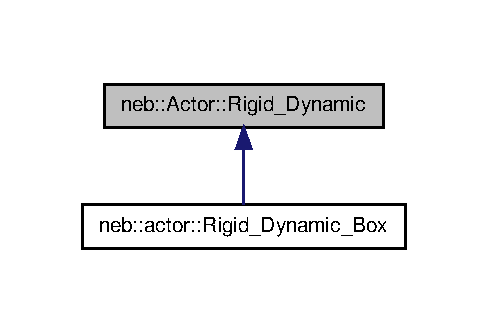
\includegraphics[width=234pt]{classneb_1_1Actor_1_1Rigid__Dynamic__inherit__graph}
\end{center}
\end{figure}
\subsection*{\-Public \-Member \-Functions}
\begin{DoxyCompactItemize}
\item 
\hypertarget{classneb_1_1Actor_1_1Rigid__Dynamic_a2e4d16eec6b3a7380d70c9d7d466e5bb}{{\bfseries \-Rigid\-\_\-\-Dynamic} (boost\-::shared\-\_\-ptr$<$ glutpp\-::actor\-::parent $>$)}\label{classneb_1_1Actor_1_1Rigid__Dynamic_a2e4d16eec6b3a7380d70c9d7d466e5bb}

\item 
\hypertarget{classneb_1_1Actor_1_1Rigid__Dynamic_aafeadc8a6f50516b73518bb01fd0dc88}{virtual void {\bfseries init} (boost\-::shared\-\_\-ptr$<$ glutpp\-::actor\-::desc $>$)}\label{classneb_1_1Actor_1_1Rigid__Dynamic_aafeadc8a6f50516b73518bb01fd0dc88}

\item 
\hypertarget{classneb_1_1Actor_1_1Rigid__Dynamic_adefdc5dc7aeaffe4f11474c6fa8dd5a7}{virtual void {\bfseries create\-\_\-physics} ()}\label{classneb_1_1Actor_1_1Rigid__Dynamic_adefdc5dc7aeaffe4f11474c6fa8dd5a7}

\item 
\hypertarget{classneb_1_1Actor_1_1Rigid__Dynamic_a8a5f3edafc98b3e0219e2f5466a96959}{virtual void {\bfseries init\-\_\-physics} ()}\label{classneb_1_1Actor_1_1Rigid__Dynamic_a8a5f3edafc98b3e0219e2f5466a96959}

\item 
\hypertarget{classneb_1_1Actor_1_1Rigid__Dynamic_a9c4b73f164c7a5699b769430bedebab4}{virtual void {\bfseries print\-\_\-info} ()}\label{classneb_1_1Actor_1_1Rigid__Dynamic_a9c4b73f164c7a5699b769430bedebab4}

\end{DoxyCompactItemize}


\-The documentation for this class was generated from the following files\-:\begin{DoxyCompactItemize}
\item 
src/\-Nebula/\-Actor/\-Rigid\-\_\-\-Dynamic.\-hpp\item 
src/\-Nebula/\-Actor/\-Rigid\-\_\-\-Dynamic.\-cpp\end{DoxyCompactItemize}

\hypertarget{classneb_1_1actor_1_1Rigid__Dynamic__Box}{
\section{neb::actor::Rigid\_\-Dynamic\_\-Box Class Reference}
\label{classneb_1_1actor_1_1Rigid__Dynamic__Box}\index{neb::actor::Rigid\_\-Dynamic\_\-Box@{neb::actor::Rigid\_\-Dynamic\_\-Box}}
}
Inheritance diagram for neb::actor::Rigid\_\-Dynamic\_\-Box::\begin{figure}[H]
\begin{center}
\leavevmode
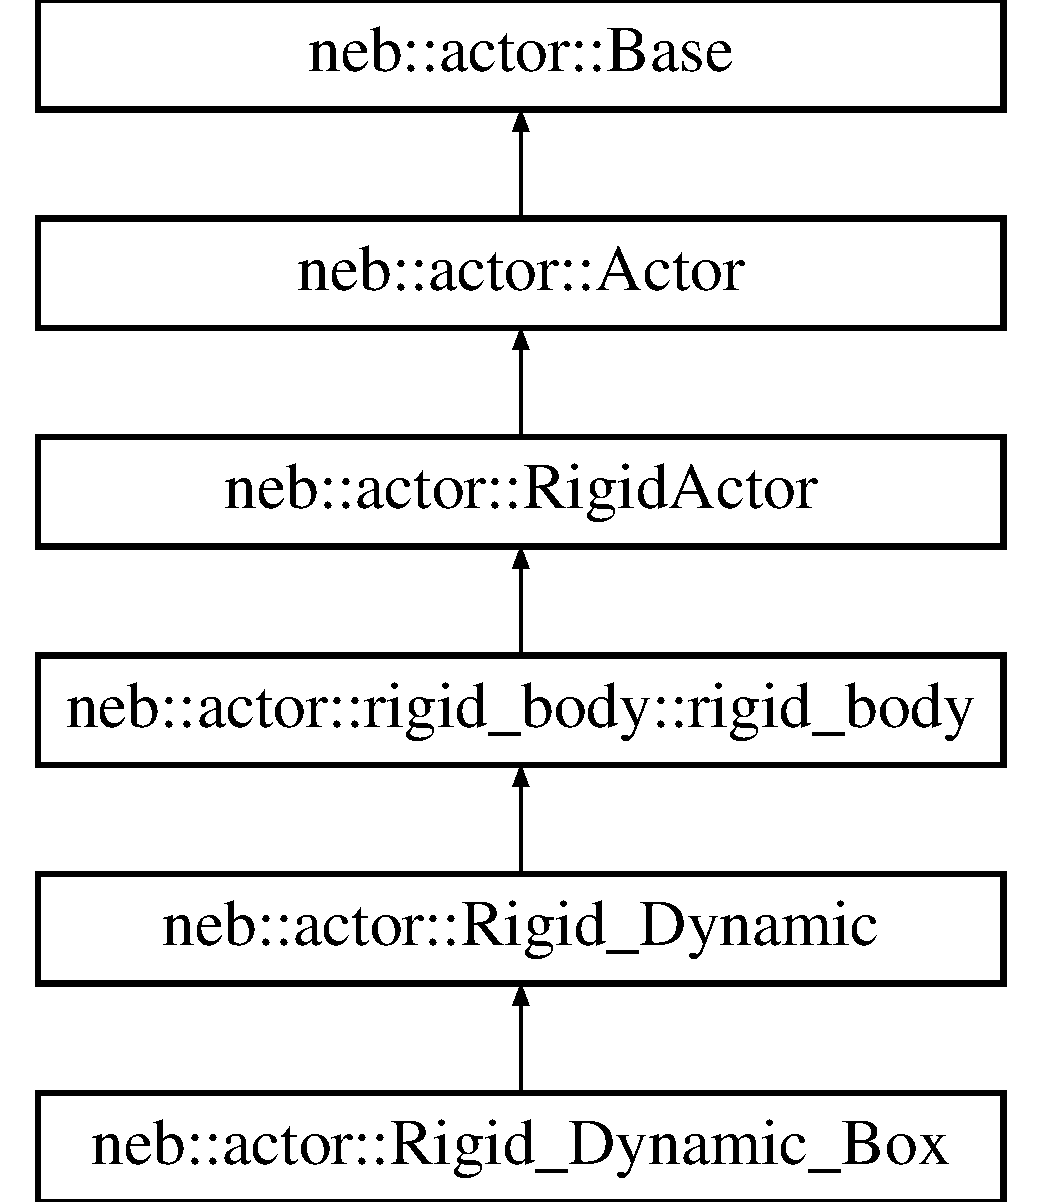
\includegraphics[height=6cm]{classneb_1_1actor_1_1Rigid__Dynamic__Box}
\end{center}
\end{figure}
\subsection*{Public Member Functions}
\begin{DoxyCompactItemize}
\item 
\hypertarget{classneb_1_1actor_1_1Rigid__Dynamic__Box_ad2564e54df3b07cc2454ba28a026b765}{
void {\bfseries Display} ()}
\label{classneb_1_1actor_1_1Rigid__Dynamic__Box_ad2564e54df3b07cc2454ba28a026b765}

\end{DoxyCompactItemize}


The documentation for this class was generated from the following file:\begin{DoxyCompactItemize}
\item 
src/nebula/actor/Rigid\_\-Dynamic\_\-Box.hpp\end{DoxyCompactItemize}

\hypertarget{classneb_1_1Actor_1_1Rigid__Static}{\section{neb\-:\-:\-Actor\-:\-:\-Rigid\-\_\-\-Static \-Class \-Reference}
\label{classneb_1_1Actor_1_1Rigid__Static}\index{neb\-::\-Actor\-::\-Rigid\-\_\-\-Static@{neb\-::\-Actor\-::\-Rigid\-\_\-\-Static}}
}
\-Inheritance diagram for neb\-:\-:\-Actor\-:\-:\-Rigid\-\_\-\-Static\-:\begin{figure}[H]
\begin{center}
\leavevmode
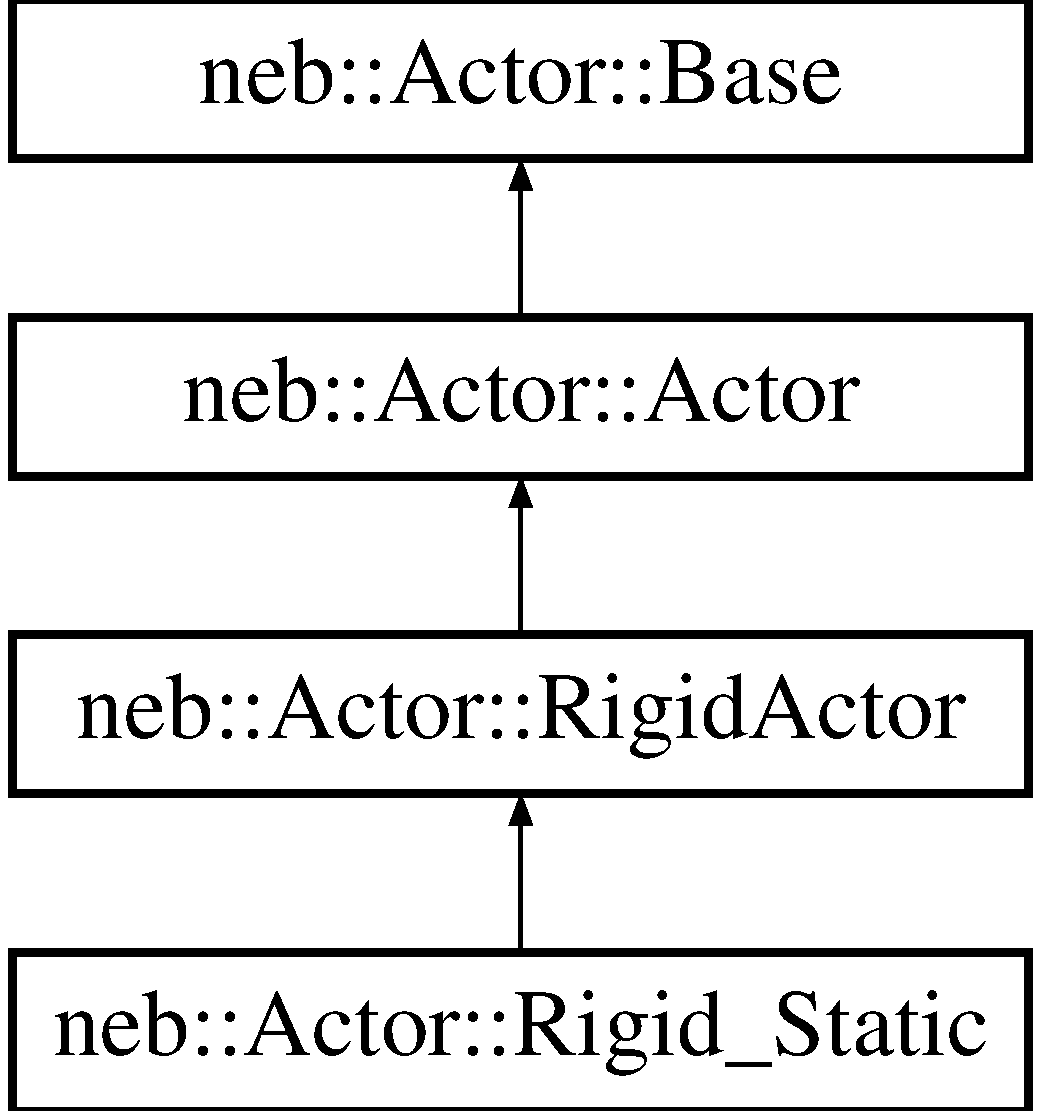
\includegraphics[height=4.000000cm]{classneb_1_1Actor_1_1Rigid__Static}
\end{center}
\end{figure}
\subsection*{\-Public \-Member \-Functions}
\begin{DoxyCompactItemize}
\item 
\hypertarget{classneb_1_1Actor_1_1Rigid__Static_a966402830e96d2a4982a845a6352b0ee}{{\bfseries \-Rigid\-\_\-\-Static} (glutpp\-::actor\-::parent\-\_\-s parent)}\label{classneb_1_1Actor_1_1Rigid__Static_a966402830e96d2a4982a845a6352b0ee}

\item 
\hypertarget{classneb_1_1Actor_1_1Rigid__Static_ab7d84259cceef7f16b9834de1ef1f2d9}{virtual void {\bfseries init} (glutpp\-::actor\-::desc\-\_\-s)}\label{classneb_1_1Actor_1_1Rigid__Static_ab7d84259cceef7f16b9834de1ef1f2d9}

\item 
\hypertarget{classneb_1_1Actor_1_1Rigid__Static_a9e8eec801df7d03445a9b4dd01fb8d67}{virtual void {\bfseries create\-\_\-physics} ()}\label{classneb_1_1Actor_1_1Rigid__Static_a9e8eec801df7d03445a9b4dd01fb8d67}

\item 
\hypertarget{classneb_1_1Actor_1_1Rigid__Static_a33c50f89376464b5f9ff2c0299fc211c}{virtual void {\bfseries init\-\_\-physics} ()}\label{classneb_1_1Actor_1_1Rigid__Static_a33c50f89376464b5f9ff2c0299fc211c}

\item 
\hypertarget{classneb_1_1Actor_1_1Rigid__Static_afca31b618b88aa4b20ca578a0a1e3a75}{virtual void {\bfseries step\-\_\-local} (double)}\label{classneb_1_1Actor_1_1Rigid__Static_afca31b618b88aa4b20ca578a0a1e3a75}

\item 
\hypertarget{classneb_1_1Actor_1_1Rigid__Static_a044fc1ffd31ca296271b00021a934ed6}{virtual void {\bfseries step\-\_\-remote} (double)}\label{classneb_1_1Actor_1_1Rigid__Static_a044fc1ffd31ca296271b00021a934ed6}

\end{DoxyCompactItemize}


\-The documentation for this class was generated from the following files\-:\begin{DoxyCompactItemize}
\item 
src/nebula/actor/\-Rigid\-\_\-\-Static.\-hpp\item 
src/nebula/actor/\-Rigid\-\_\-\-Static.\-cpp\end{DoxyCompactItemize}

\hypertarget{classneb_1_1Actor_1_1RigidActor}{\section{neb\-:\-:\-Actor\-:\-:\-Rigid\-Actor \-Class \-Reference}
\label{classneb_1_1Actor_1_1RigidActor}\index{neb\-::\-Actor\-::\-Rigid\-Actor@{neb\-::\-Actor\-::\-Rigid\-Actor}}
}
\-Inheritance diagram for neb\-:\-:\-Actor\-:\-:\-Rigid\-Actor\-:\begin{figure}[H]
\begin{center}
\leavevmode
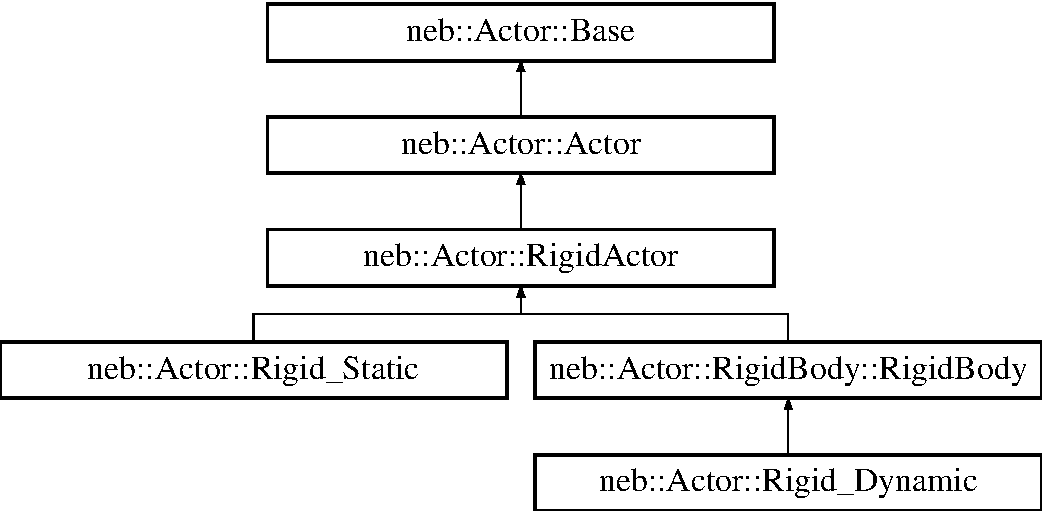
\includegraphics[height=5.000000cm]{classneb_1_1Actor_1_1RigidActor}
\end{center}
\end{figure}
\subsection*{\-Public \-Member \-Functions}
\begin{DoxyCompactItemize}
\item 
\hypertarget{classneb_1_1Actor_1_1RigidActor_ac4ff1c2a8d278a0150b78eb8f0926242}{{\bfseries \-Rigid\-Actor} (glutpp\-::actor\-::parent\-\_\-s)}\label{classneb_1_1Actor_1_1RigidActor_ac4ff1c2a8d278a0150b78eb8f0926242}

\item 
\hypertarget{classneb_1_1Actor_1_1RigidActor_a14c131b0620a383c1bac6f31903bd2c6}{virtual void {\bfseries init} (glutpp\-::actor\-::desc\-\_\-s)}\label{classneb_1_1Actor_1_1RigidActor_a14c131b0620a383c1bac6f31903bd2c6}

\item 
\hypertarget{classneb_1_1Actor_1_1RigidActor_aa46996a108d191eaa0c05beabe8ba015}{virtual void {\bfseries add\-\_\-force} (double)}\label{classneb_1_1Actor_1_1RigidActor_aa46996a108d191eaa0c05beabe8ba015}

\item 
\hypertarget{classneb_1_1Actor_1_1RigidActor_ab387292054623de9ec9c5de26ad84d71}{virtual void {\bfseries step\-\_\-local} (double)}\label{classneb_1_1Actor_1_1RigidActor_ab387292054623de9ec9c5de26ad84d71}

\item 
\hypertarget{classneb_1_1Actor_1_1RigidActor_ab72bf9a60632e398f601b0f1adbf811e}{virtual void {\bfseries step\-\_\-remote} (double)}\label{classneb_1_1Actor_1_1RigidActor_ab72bf9a60632e398f601b0f1adbf811e}

\item 
\hypertarget{classneb_1_1Actor_1_1RigidActor_a0c859ee3609c13faf5f626b9aa6f67ab}{virtual void {\bfseries setup\-Filtering} ()}\label{classneb_1_1Actor_1_1RigidActor_a0c859ee3609c13faf5f626b9aa6f67ab}

\item 
\hypertarget{classneb_1_1Actor_1_1RigidActor_affb958ff8ac655c25906b0a9cd0f0bb5}{virtual glutpp\-::actor\-::desc\-\_\-s {\bfseries get\-\_\-projectile} ()}\label{classneb_1_1Actor_1_1RigidActor_affb958ff8ac655c25906b0a9cd0f0bb5}

\item 
\hypertarget{classneb_1_1Actor_1_1RigidActor_ae43181ba4f6b5b3fb782f6a689ec5dc5}{virtual void {\bfseries create\-\_\-physics} ()}\label{classneb_1_1Actor_1_1RigidActor_ae43181ba4f6b5b3fb782f6a689ec5dc5}

\item 
\hypertarget{classneb_1_1Actor_1_1RigidActor_a558079bb45a9986bfbfcb92c2d8e005a}{virtual void {\bfseries init\-\_\-physics} ()}\label{classneb_1_1Actor_1_1RigidActor_a558079bb45a9986bfbfcb92c2d8e005a}

\item 
\hypertarget{classneb_1_1Actor_1_1RigidActor_a8dd99df00071772dfd5227226105a16e}{virtual void {\bfseries print\-\_\-info} ()}\label{classneb_1_1Actor_1_1RigidActor_a8dd99df00071772dfd5227226105a16e}

\end{DoxyCompactItemize}


\-The documentation for this class was generated from the following files\-:\begin{DoxyCompactItemize}
\item 
src/nebula/actor/\-Rigid\-\_\-\-Actor.\-hpp\item 
src/nebula/actor/\-Rigid\-\_\-\-Actor.\-cpp\end{DoxyCompactItemize}

\hypertarget{classneb_1_1Actor_1_1RigidBody_1_1RigidBody}{
\section{neb::Actor::RigidBody::RigidBody Class Reference}
\label{classneb_1_1Actor_1_1RigidBody_1_1RigidBody}\index{neb::Actor::RigidBody::RigidBody@{neb::Actor::RigidBody::RigidBody}}
}
\subsection*{Public Member Functions}
\begin{DoxyCompactItemize}
\item 
\hypertarget{classneb_1_1Actor_1_1RigidBody_1_1RigidBody_a4a42b50cdc34ed40704fe68a6044aac5}{
{\bfseries RigidBody} (glutpp::actor::parent\_\-s)}
\label{classneb_1_1Actor_1_1RigidBody_1_1RigidBody_a4a42b50cdc34ed40704fe68a6044aac5}

\item 
\hypertarget{classneb_1_1Actor_1_1RigidBody_1_1RigidBody_a49bc7986eea3d48486dc8bdba8b84954}{
virtual void {\bfseries init} (glutpp::actor::desc\_\-s)}
\label{classneb_1_1Actor_1_1RigidBody_1_1RigidBody_a49bc7986eea3d48486dc8bdba8b84954}

\item 
\hypertarget{classneb_1_1Actor_1_1RigidBody_1_1RigidBody_af9d4be08596daf414fc020ac6c659a6e}{
virtual glutpp::actor::desc\_\-s {\bfseries get\_\-projectile} ()}
\label{classneb_1_1Actor_1_1RigidBody_1_1RigidBody_af9d4be08596daf414fc020ac6c659a6e}

\item 
\hypertarget{classneb_1_1Actor_1_1RigidBody_1_1RigidBody_a113a8004e1564ce207c89101bb015086}{
virtual void {\bfseries print\_\-info} ()}
\label{classneb_1_1Actor_1_1RigidBody_1_1RigidBody_a113a8004e1564ce207c89101bb015086}

\item 
\hypertarget{classneb_1_1Actor_1_1RigidBody_1_1RigidBody_a690d134f35e34636883622d13596592c}{
virtual void {\bfseries create\_\-physics} ()}
\label{classneb_1_1Actor_1_1RigidBody_1_1RigidBody_a690d134f35e34636883622d13596592c}

\item 
\hypertarget{classneb_1_1Actor_1_1RigidBody_1_1RigidBody_a5217679a926c4bdbd9006545751c39ac}{
virtual void {\bfseries create\_\-control} (neb::control::rigid\_\-body::raw\_\-s)}
\label{classneb_1_1Actor_1_1RigidBody_1_1RigidBody_a5217679a926c4bdbd9006545751c39ac}

\end{DoxyCompactItemize}
\subsection*{Public Attributes}
\begin{DoxyCompactItemize}
\item 
\hypertarget{classneb_1_1Actor_1_1RigidBody_1_1RigidBody_a873b6a4d9a88f20b12cbae77aeed5607}{
neb::control::rigid\_\-body::control\_\-s {\bfseries control\_\-}}
\label{classneb_1_1Actor_1_1RigidBody_1_1RigidBody_a873b6a4d9a88f20b12cbae77aeed5607}

\end{DoxyCompactItemize}


The documentation for this class was generated from the following file:\begin{DoxyCompactItemize}
\item 
src/nebula/actor/rigid\_\-body/rigid\_\-body.hpp\end{DoxyCompactItemize}

\hypertarget{classneb_1_1scene_1_1scene}{\section{neb\-:\-:scene\-:\-:scene \-Class \-Reference}
\label{classneb_1_1scene_1_1scene}\index{neb\-::scene\-::scene@{neb\-::scene\-::scene}}
}
\subsection*{\-Public \-Types}
\begin{DoxyCompactItemize}
\item 
enum \{ {\bfseries \-N\-O\-N\-E} =  0, 
{\bfseries \-L\-O\-C\-A\-L}, 
{\bfseries \-R\-E\-M\-O\-T\-E}
 \}
\item 
\hypertarget{classneb_1_1scene_1_1scene_a93173acffbdc556f0a641cd221c54a5a}{typedef std\-::shared\-\_\-ptr\*
$<$ \hyperlink{classneb_1_1Actor_1_1Base}{neb\-::\-Actor\-::\-Base} $>$ {\bfseries base\-\_\-t}}\label{classneb_1_1scene_1_1scene_a93173acffbdc556f0a641cd221c54a5a}

\item 
\hypertarget{classneb_1_1scene_1_1scene_a67e04f8f35aa73c9fd192d9c4fbe403c}{typedef std\-::shared\-\_\-ptr\*
$<$ \hyperlink{classneb_1_1Actor_1_1Rigid__Dynamic}{neb\-::\-Actor\-::\-Rigid\-\_\-\-Dynamic} $>$ {\bfseries rigid\-\_\-dynamic\-\_\-t}}\label{classneb_1_1scene_1_1scene_a67e04f8f35aa73c9fd192d9c4fbe403c}

\item 
\hypertarget{classneb_1_1scene_1_1scene_a5ffbe126690d92a6a21821b5770f085e}{typedef std\-::shared\-\_\-ptr\*
$<$ \hyperlink{classneb_1_1Actor_1_1Rigid__Static}{neb\-::\-Actor\-::\-Rigid\-\_\-\-Static} $>$ {\bfseries rigid\-\_\-static\-\_\-t}}\label{classneb_1_1scene_1_1scene_a5ffbe126690d92a6a21821b5770f085e}

\item 
\hypertarget{classneb_1_1scene_1_1scene_afbea2ea9e297eb5a6b35e94ab71555b8}{typedef std\-::shared\-\_\-ptr\*
$<$ \hyperlink{classneb_1_1Actor_1_1Controller}{neb\-::\-Actor\-::\-Controller} $>$ {\bfseries controller\-\_\-t}}\label{classneb_1_1scene_1_1scene_afbea2ea9e297eb5a6b35e94ab71555b8}

\item 
\hypertarget{classneb_1_1scene_1_1scene_a91d267e955478e0ae15693eb49103e3c}{typedef std\-::shared\-\_\-ptr$<$ \hyperlink{classneb_1_1app}{neb\-::app} $>$ {\bfseries app\-\_\-t}}\label{classneb_1_1scene_1_1scene_a91d267e955478e0ae15693eb49103e3c}

\end{DoxyCompactItemize}
\subsection*{\-Public \-Member \-Functions}
\begin{DoxyCompactItemize}
\item 
\hypertarget{classneb_1_1scene_1_1scene_abccb582576f45ce1b923bf6b6a153da6}{{\bfseries scene} (neb\-::app\-\_\-s)}\label{classneb_1_1scene_1_1scene_abccb582576f45ce1b923bf6b6a153da6}

\item 
\hypertarget{classneb_1_1scene_1_1scene_a44f7744f9e07ad6a8722689b3f8392b4}{void {\bfseries init} (glutpp\-::scene\-::desc\-\_\-s)}\label{classneb_1_1scene_1_1scene_a44f7744f9e07ad6a8722689b3f8392b4}

\item 
\hypertarget{classneb_1_1scene_1_1scene_a86d094b5dfff986da693d385c0f0f245}{void {\bfseries create\-\_\-physics} ()}\label{classneb_1_1scene_1_1scene_a86d094b5dfff986da693d385c0f0f245}

\item 
\hypertarget{classneb_1_1scene_1_1scene_a4a18d76291ad008be51b7fb8b22f1451}{app\-\_\-t {\bfseries get\-\_\-app} ()}\label{classneb_1_1scene_1_1scene_a4a18d76291ad008be51b7fb8b22f1451}

\item 
\hypertarget{classneb_1_1scene_1_1scene_aa6b526a0dfec00fa2ae1add784cf05f4}{base\-\_\-t {\bfseries get\-\_\-actor} (int i)}\label{classneb_1_1scene_1_1scene_aa6b526a0dfec00fa2ae1add784cf05f4}

\item 
\hypertarget{classneb_1_1scene_1_1scene_a70668d15ace0a19fb99f2a7de7b56b0d}{base\-\_\-t {\bfseries get\-\_\-actor} (glutpp\-::actor\-::addr\-\_\-s)}\label{classneb_1_1scene_1_1scene_a70668d15ace0a19fb99f2a7de7b56b0d}

\item 
\hypertarget{classneb_1_1scene_1_1scene_ad407feafc7a6378d8c05bbe7e0bd65df}{void {\bfseries create\-\_\-actors} (glutpp\-::scene\-::desc\-\_\-s)}\label{classneb_1_1scene_1_1scene_ad407feafc7a6378d8c05bbe7e0bd65df}

\item 
\hypertarget{classneb_1_1scene_1_1scene_a05681da591d690465575e63fbf192f6e}{base\-\_\-t {\bfseries create\-\_\-actor\-\_\-local} (glutpp\-::actor\-::desc\-\_\-s)}\label{classneb_1_1scene_1_1scene_a05681da591d690465575e63fbf192f6e}

\item 
\hypertarget{classneb_1_1scene_1_1scene_afe04b4b8f4d397595414c705a9ee751d}{base\-\_\-t {\bfseries create\-\_\-actor\-\_\-remote} (glutpp\-::actor\-::addr\-\_\-s, glutpp\-::actor\-::desc\-\_\-s)}\label{classneb_1_1scene_1_1scene_afe04b4b8f4d397595414c705a9ee751d}

\item 
\hypertarget{classneb_1_1scene_1_1scene_a5afc16565aeba302bcb42829499d263f}{void {\bfseries add\-\_\-deferred} (glutpp\-::actor\-::desc\-\_\-s)}\label{classneb_1_1scene_1_1scene_a5afc16565aeba302bcb42829499d263f}

\item 
\hypertarget{classneb_1_1scene_1_1scene_ad7ec98ad9a99bf3085c26da967e5b5ea}{void {\bfseries draw} ()}\label{classneb_1_1scene_1_1scene_ad7ec98ad9a99bf3085c26da967e5b5ea}

\item 
\hypertarget{classneb_1_1scene_1_1scene_abc55b6d1ba97b57881d0830f0121b11c}{void {\bfseries step} (double)}\label{classneb_1_1scene_1_1scene_abc55b6d1ba97b57881d0830f0121b11c}

\item 
\hypertarget{classneb_1_1scene_1_1scene_a93c887dbb7f649c7c93383777f98715e}{void {\bfseries step\-\_\-local} (double)}\label{classneb_1_1scene_1_1scene_a93c887dbb7f649c7c93383777f98715e}

\item 
\hypertarget{classneb_1_1scene_1_1scene_a897abb36acc753cb589bbf58b8603767}{void {\bfseries step\-\_\-remote} (double)}\label{classneb_1_1scene_1_1scene_a897abb36acc753cb589bbf58b8603767}

\item 
\hypertarget{classneb_1_1scene_1_1scene_ab0240c3bcde1ab4ee7cf9b5cc072f22e}{void {\bfseries fire} (neb\-::\-Actor\-::\-Base\-\_\-s)}\label{classneb_1_1scene_1_1scene_ab0240c3bcde1ab4ee7cf9b5cc072f22e}

\item 
void \hyperlink{classneb_1_1scene_1_1scene_a28b7352c7b6898b4d1bc20aae31d7443}{fire\-\_\-local} (neb\-::\-Actor\-::\-Base\-\_\-s)
\item 
\hypertarget{classneb_1_1scene_1_1scene_ac73e5d6ff905bce7fb031a39fd3180c8}{void {\bfseries fire\-\_\-remote} (neb\-::\-Actor\-::\-Base\-\_\-s)}\label{classneb_1_1scene_1_1scene_ac73e5d6ff905bce7fb031a39fd3180c8}

\item 
\hypertarget{classneb_1_1scene_1_1scene_acbac0a7094a148af1fe709bffb0589c1}{math\-::mat44 {\bfseries get\-Pose} ()}\label{classneb_1_1scene_1_1scene_acbac0a7094a148af1fe709bffb0589c1}

\item 
\hypertarget{classneb_1_1scene_1_1scene_a50132e0e00ed5707017f27308b1784cf}{math\-::mat44 {\bfseries get\-Pose\-Global} ()}\label{classneb_1_1scene_1_1scene_a50132e0e00ed5707017f27308b1784cf}

\item 
\hypertarget{classneb_1_1scene_1_1scene_abc96c584a43aabbb6e4bc8d66ed35a2a}{void {\bfseries send\-\_\-actor\-\_\-update} ()}\label{classneb_1_1scene_1_1scene_abc96c584a43aabbb6e4bc8d66ed35a2a}

\item 
\hypertarget{classneb_1_1scene_1_1scene_a037bc8e01e290d9c1fc6959a13343c1e}{virtual void {\bfseries dumby} ()}\label{classneb_1_1scene_1_1scene_a037bc8e01e290d9c1fc6959a13343c1e}

\end{DoxyCompactItemize}
\subsection*{\-Public \-Attributes}
\begin{DoxyCompactItemize}
\item 
\hypertarget{classneb_1_1scene_1_1scene_a8527e6bb51b445c7dc99efcaaa8198c1}{neb\-::app\-\_\-w {\bfseries app\-\_\-}}\label{classneb_1_1scene_1_1scene_a8527e6bb51b445c7dc99efcaaa8198c1}

\item 
\hypertarget{classneb_1_1scene_1_1scene_a99398d74631477541fe414f7455c6560}{gal\-::timer\-::timer\-\_\-set {\bfseries timer\-\_\-set\-\_\-}}\label{classneb_1_1scene_1_1scene_a99398d74631477541fe414f7455c6560}

\item 
\hypertarget{classneb_1_1scene_1_1scene_a0c7cc06520332f35eaaa43d06f303e17}{int {\bfseries user\-\_\-type\-\_\-}}\label{classneb_1_1scene_1_1scene_a0c7cc06520332f35eaaa43d06f303e17}

\item 
\hypertarget{classneb_1_1scene_1_1scene_a4080cb2f22531e88d5562834011dd8e0}{physx\-::\-Px\-Simulation\-Filter\-Shader {\bfseries px\-\_\-filter\-\_\-shader\-\_\-}}\label{classneb_1_1scene_1_1scene_a4080cb2f22531e88d5562834011dd8e0}

\item 
\hypertarget{classneb_1_1scene_1_1scene_a65cada9f46dc732db546eff588c9eae8}{\hyperlink{classneb_1_1simulation__callback}{neb\-::simulation\-\_\-callback} $\ast$ {\bfseries simulation\-\_\-callback\-\_\-}}\label{classneb_1_1scene_1_1scene_a65cada9f46dc732db546eff588c9eae8}

\item 
\hypertarget{classneb_1_1scene_1_1scene_a94b89a56deddecfba35b9829f8315ad8}{physx\-::\-Px\-Scene $\ast$ {\bfseries px\-\_\-scene\-\_\-}}\label{classneb_1_1scene_1_1scene_a94b89a56deddecfba35b9829f8315ad8}

\item 
\hypertarget{classneb_1_1scene_1_1scene_a37110b74e5abbe2e88c92815f533a937}{double {\bfseries last\-\_\-}}\label{classneb_1_1scene_1_1scene_a37110b74e5abbe2e88c92815f533a937}

\end{DoxyCompactItemize}


\subsection{\-Member \-Function \-Documentation}
\hypertarget{classneb_1_1scene_1_1scene_a28b7352c7b6898b4d1bc20aae31d7443}{\index{neb\-::scene\-::scene@{neb\-::scene\-::scene}!fire\-\_\-local@{fire\-\_\-local}}
\index{fire\-\_\-local@{fire\-\_\-local}!neb::scene::scene@{neb\-::scene\-::scene}}
\subsubsection[{fire\-\_\-local}]{\setlength{\rightskip}{0pt plus 5cm}void {\bf neb\-::scene\-::scene\-::fire\-\_\-local} (
\begin{DoxyParamCaption}
\item[{neb\-::\-Actor\-::\-Base\-\_\-s}]{actor}
\end{DoxyParamCaption}
)}}\label{classneb_1_1scene_1_1scene_a28b7352c7b6898b4d1bc20aae31d7443}
\begin{DoxyRefDesc}{\-Todo}
\item[\hyperlink{todo__todo000001}{\-Todo}]replace neb\-::timer\-::actor\-::type with inheritance \end{DoxyRefDesc}


\-The documentation for this class was generated from the following files\-:\begin{DoxyCompactItemize}
\item 
src/nebula/scene/scene.\-hpp\item 
src/nebula/scene/scene.\-cpp\end{DoxyCompactItemize}

\hypertarget{classneb_1_1network_1_1server}{
\section{neb::network::server Class Reference}
\label{classneb_1_1network_1_1server}\index{neb::network::server@{neb::network::server}}
}
\subsection*{Public Member Functions}
\begin{DoxyCompactItemize}
\item 
\hypertarget{classneb_1_1network_1_1server_a55eb2c80a90c0b5b6d858373b8162ec4}{
{\bfseries server} (neb::app\_\-s, unsigned short, int)}
\label{classneb_1_1network_1_1server_a55eb2c80a90c0b5b6d858373b8162ec4}

\item 
\hypertarget{classneb_1_1network_1_1server_a3abc21bea913d905137668449665e7c4}{
void {\bfseries callback\_\-accept} (int)}
\label{classneb_1_1network_1_1server_a3abc21bea913d905137668449665e7c4}

\end{DoxyCompactItemize}
\subsection*{Public Attributes}
\begin{DoxyCompactItemize}
\item 
\hypertarget{classneb_1_1network_1_1server_a878fe2bc88c7e06dcd6b88d6dc0a5983}{
std::weak\_\-ptr$<$ \hyperlink{classneb_1_1app}{neb::app} $>$ {\bfseries app\_\-}}
\label{classneb_1_1network_1_1server_a878fe2bc88c7e06dcd6b88d6dc0a5983}

\end{DoxyCompactItemize}


The documentation for this class was generated from the following files:\begin{DoxyCompactItemize}
\item 
src/nebula/network/server.hpp\item 
src/nebula/network/server.cpp\end{DoxyCompactItemize}

\hypertarget{classneb_1_1shape_1_1shape}{\section{neb\-:\-:shape\-:\-:shape \-Class \-Reference}
\label{classneb_1_1shape_1_1shape}\index{neb\-::shape\-::shape@{neb\-::shape\-::shape}}
}
\subsection*{\-Public \-Member \-Functions}
\begin{DoxyCompactItemize}
\item 
\hypertarget{classneb_1_1shape_1_1shape_a99b6ce85fd11ae4c653af5d224eccf0e}{{\bfseries shape} (glutpp\-::shape\-::parent\-\_\-s)}\label{classneb_1_1shape_1_1shape_a99b6ce85fd11ae4c653af5d224eccf0e}

\item 
\hypertarget{classneb_1_1shape_1_1shape_a6b32b64391220f5b23eabe7f9c4af596}{virtual void {\bfseries init} (glutpp\-::shape\-::desc\-\_\-s)}\label{classneb_1_1shape_1_1shape_a6b32b64391220f5b23eabe7f9c4af596}

\item 
\hypertarget{classneb_1_1shape_1_1shape_af34910feff0944f03ce5a0cd7599f956}{void {\bfseries create\-\_\-physics} ()}\label{classneb_1_1shape_1_1shape_af34910feff0944f03ce5a0cd7599f956}

\item 
\hypertarget{classneb_1_1shape_1_1shape_a6c52cdce2b3575c73d9440fba5e6934e}{physx\-::\-Px\-Geometry $\ast$ {\bfseries to\-\_\-geo} ()}\label{classneb_1_1shape_1_1shape_a6c52cdce2b3575c73d9440fba5e6934e}

\item 
\hypertarget{classneb_1_1shape_1_1shape_ae89b01dc51c8d11d478c4377d5cea38c}{void {\bfseries print\-\_\-info} ()}\label{classneb_1_1shape_1_1shape_ae89b01dc51c8d11d478c4377d5cea38c}

\end{DoxyCompactItemize}
\subsection*{\-Public \-Attributes}
\begin{DoxyCompactItemize}
\item 
\hypertarget{classneb_1_1shape_1_1shape_aede64cf428691b049d68c5f62fd22383}{physx\-::\-Px\-Shape $\ast$ {\bfseries px\-\_\-shape\-\_\-}}\label{classneb_1_1shape_1_1shape_aede64cf428691b049d68c5f62fd22383}

\end{DoxyCompactItemize}


\-The documentation for this class was generated from the following files\-:\begin{DoxyCompactItemize}
\item 
src/nebula/shape.\-hpp\item 
src/nebula/shape.\-cpp\end{DoxyCompactItemize}

\hypertarget{classneb_1_1simulation__callback}{\section{neb\-:\-:simulation\-\_\-callback \-Class \-Reference}
\label{classneb_1_1simulation__callback}\index{neb\-::simulation\-\_\-callback@{neb\-::simulation\-\_\-callback}}
}
\subsection*{\-Public \-Member \-Functions}
\begin{DoxyCompactItemize}
\item 
\hypertarget{classneb_1_1simulation__callback_a19793cdc33472be18f7839fb2d7fea97}{virtual void {\bfseries on\-Constraint\-Break} (physx\-::\-Px\-Constraint\-Info $\ast$constraints, physx\-::\-Px\-U32 count)}\label{classneb_1_1simulation__callback_a19793cdc33472be18f7839fb2d7fea97}

\item 
\hypertarget{classneb_1_1simulation__callback_ae3c155b2b77603562be48c4e67fa8026}{virtual void {\bfseries on\-Wake} (physx\-::\-Px\-Actor $\ast$$\ast$actors, physx\-::\-Px\-U32 count)}\label{classneb_1_1simulation__callback_ae3c155b2b77603562be48c4e67fa8026}

\item 
\hypertarget{classneb_1_1simulation__callback_ab5f0852a4102fc6adf5a981803b11fc9}{virtual void {\bfseries on\-Sleep} (physx\-::\-Px\-Actor $\ast$$\ast$actors, physx\-::\-Px\-U32 count)}\label{classneb_1_1simulation__callback_ab5f0852a4102fc6adf5a981803b11fc9}

\item 
\hypertarget{classneb_1_1simulation__callback_a81d02ce1df83fbec396560c9f250e9a1}{virtual void {\bfseries on\-Contact} (const physx\-::\-Px\-Contact\-Pair\-Header \&pair\-Header, const physx\-::\-Px\-Contact\-Pair $\ast$pairs, physx\-::\-Px\-U32 nb\-Pairs)}\label{classneb_1_1simulation__callback_a81d02ce1df83fbec396560c9f250e9a1}

\item 
\hypertarget{classneb_1_1simulation__callback_a380b0166d2a5313df0a257960f069672}{virtual void {\bfseries on\-Trigger} (physx\-::\-Px\-Trigger\-Pair $\ast$pairs, physx\-::\-Px\-U32 count)}\label{classneb_1_1simulation__callback_a380b0166d2a5313df0a257960f069672}

\end{DoxyCompactItemize}


\-The documentation for this class was generated from the following files\-:\begin{DoxyCompactItemize}
\item 
src/nebula/simulation\-\_\-callback.\-hpp\item 
src/nebula/simulation\-\_\-callback.\-cpp\end{DoxyCompactItemize}

\hypertarget{classneb_1_1network_1_1control_1_1rigid__body_1_1update}{\section{neb\-:\-:network\-:\-:control\-:\-:rigid\-\_\-body\-:\-:update \-Class \-Reference}
\label{classneb_1_1network_1_1control_1_1rigid__body_1_1update}\index{neb\-::network\-::control\-::rigid\-\_\-body\-::update@{neb\-::network\-::control\-::rigid\-\_\-body\-::update}}
}
\subsection*{\-Public \-Member \-Functions}
\begin{DoxyCompactItemize}
\item 
\hypertarget{classneb_1_1network_1_1control_1_1rigid__body_1_1update_a4dbab97fac5f7d43af6c6bcb96f5f36f}{glutpp\-::actor\-::addr\-\_\-s {\bfseries get\-\_\-addr} ()}\label{classneb_1_1network_1_1control_1_1rigid__body_1_1update_a4dbab97fac5f7d43af6c6bcb96f5f36f}

\item 
\hypertarget{classneb_1_1network_1_1control_1_1rigid__body_1_1update_ab176f1660a245cb5789e5f923c056843}{neb\-::control\-::rigid\-\_\-body\-::raw\-\_\-s {\bfseries get\-\_\-raw} ()}\label{classneb_1_1network_1_1control_1_1rigid__body_1_1update_ab176f1660a245cb5789e5f923c056843}

\end{DoxyCompactItemize}


\-The documentation for this class was generated from the following file\-:\begin{DoxyCompactItemize}
\item 
src/nebula/network/message.\-hpp\end{DoxyCompactItemize}

\hypertarget{classneb_1_1user}{\section{neb\-:\-:user \-Class \-Reference}
\label{classneb_1_1user}\index{neb\-::user@{neb\-::user}}
}
\subsection*{\-Public \-Member \-Functions}
\begin{DoxyCompactItemize}
\item 
\hypertarget{classneb_1_1user_a03537b4a3dbb21efa368fcf846384dd5}{void {\bfseries init} ()}\label{classneb_1_1user_a03537b4a3dbb21efa368fcf846384dd5}

\item 
\hypertarget{classneb_1_1user_a4bbd0003c3ba2ef7f25579784cbcb6f5}{void {\bfseries connect} (glutpp\-::window\-::window\-\_\-s)}\label{classneb_1_1user_a4bbd0003c3ba2ef7f25579784cbcb6f5}

\item 
\hypertarget{classneb_1_1user_ae6295dcc8ac8e664cedc8591c28257d0}{void {\bfseries set\-\_\-control} (neb\-::control\-::rigid\-\_\-body\-::control\-\_\-s)}\label{classneb_1_1user_ae6295dcc8ac8e664cedc8591c28257d0}

\end{DoxyCompactItemize}
\subsection*{\-Public \-Attributes}
\begin{DoxyCompactItemize}
\item 
\hypertarget{classneb_1_1user_a66992175b55bcc61803d87d19f1327f8}{neb\-::control\-::rigid\-\_\-body\-::control\-\_\-s {\bfseries control\-\_\-}}\label{classneb_1_1user_a66992175b55bcc61803d87d19f1327f8}

\end{DoxyCompactItemize}


\-The documentation for this class was generated from the following files\-:\begin{DoxyCompactItemize}
\item 
src/\-Nebula/user.\-hpp\item 
src/\-Nebula/user.\-cpp\end{DoxyCompactItemize}

\printindex
\end{document}
